\documentclass[11pt]{article}

\usepackage[margin=1in]{geometry}
\usepackage{setspace}
\onehalfspacing
\usepackage{graphicx}
\graphicspath{report_images/}
\usepackage{appendix}
\usepackage{listings}
\usepackage{float}
\usepackage{multirow}
\usepackage{amsthm}
% The next three lines make the table and figure numbers also include section number
\usepackage{chngcntr}
\counterwithin{table}{section}
\counterwithin{figure}{section}
% Needed to make titling page without a page number
\usepackage{titling}

% DOCUMENT INFORMATION =================================================
\font\titleFont=cmr12 at 11pt
\title {{\titleFont ECEN 429: Introduction to Digital Systems Design Laboratory \\ North Carolina Agricultural and Technical State University \\ Department of Electrical and Computer Engineering}} % Declare Title
\author{\titleFont Reporter: Chris Cannon\\ \titleFont Partner: Nikiyah Beulah} % Declare authors
\date{\titleFont March 1, 2018}
% ======================================================================

\begin{document}

\begin{titlingpage}
\maketitle
\begin{center}
	Lab 7
\end{center}
\end{titlingpage}

\section{Introduction}
This lab tests our ability to integrate multiple, relatively complex synchronous devices into a single unit. When complete, this lab will produce a finite state machine that will conduct arithmetic operations in each state.

\theoremstyle{definition}
\newtheorem{definition}{Definition}
\begin{definition}
Synchronous Device: an electronic circuit that performs operations in time with a clock.
\label{def:synchronous_device}
\end{definition}

\section{Background, Design Solution, and Results}

\subsection{Problem 1 }

\subsubsection{Background}
For Problem 1, we were to complete an ALU that would perform operations on 2 2-bit operands. We were instructed to select 4 operations for our ALU to complete, and we chose $AND, OR, LOGICAL SHIFT LEFT,$ and $LOGICAL SHIFT RIGHT$.

\subsubsection{Design Solution}
We decided to design individual entities for each arithmetic operation that we wished to complete. The thought process behind this design is that it will reduce the complexity of our overall code as well as run faster because we are simulating separate hardware for each operation to be completed. Because the inputs are 2-bits, the output will be 2-bits only. All overflow will be ignored, and negative numbers will be displayed as "00". Inputs for this system is assigned in Table ~\ref{tab:alu_input_Ports} and outputs are assigned in Table ~\ref{tab:alu_output_Ports}. A different operation will be performed for each possible value of the select input SEL, and those operations are defined in Table ~\ref{tab:alu_sel_ops}.

\begin{table}[H]
\begin{center}
\begin{tabular}{| l | l | l |}
	\hline
	Bit & Label & Port \\ \hline
	in1[0] &  Switch 5 & V15 \\ \hline
	in1[1] & Switch 4 & w15 \\ \hline
	in2[0] & Switch 3 & W16 \\ \hline
	in2[1] & Switch 2 & W17 \\ \hline
	sel[0] & Switch 1 & U19 \\ \hline
	sel[1] & Switch 0 & V16 \\ \hline
\end{tabular}
\caption{\label{tab:alu_input_Ports}Input port assignments for  the arithmetic logic unit.}
\end{center}
\end{table}

\begin{table}[H]
\begin{center}
\begin{tabular}{| l | l | l |}
	\hline
	Bit & Label & Port \\ \hline
	output[0] & LED 0 & U16 \\ \hline
	output[1] & LED 1 & E19 \\ \hline
\end{tabular}
\caption{\label{tab:alu_output_Ports}Output port assignments for arithmetic logic unit.}
\end{center}
\end{table}

\begin{table}[H]
\begin{center}
\begin{tabular}{| l | l |}
	\hline
	SEL & Operation \\ \hline
	"00" & $output = in1 AND in2$ \\ \hline
	"01" & $output = in1 OR in2$ \\ \hline
	"10" & $output = in1 SHIFT_RIGHT_BY in2 BITS$ \\ \hline
	"11" & $output = in1 SHIFT_LEFT_BY in2 BITS$ \\ \hline
\end{tabular}
\caption{\label{tab:alu_sel_ops}Operation performed for a given select input SEL.}
\end{center}
\end{table}

\subsubsection{Results}
Our arithmetic logic unit operated as expected and results are shown in the figures below.

\begin{figure}[H]
\begin{center}
	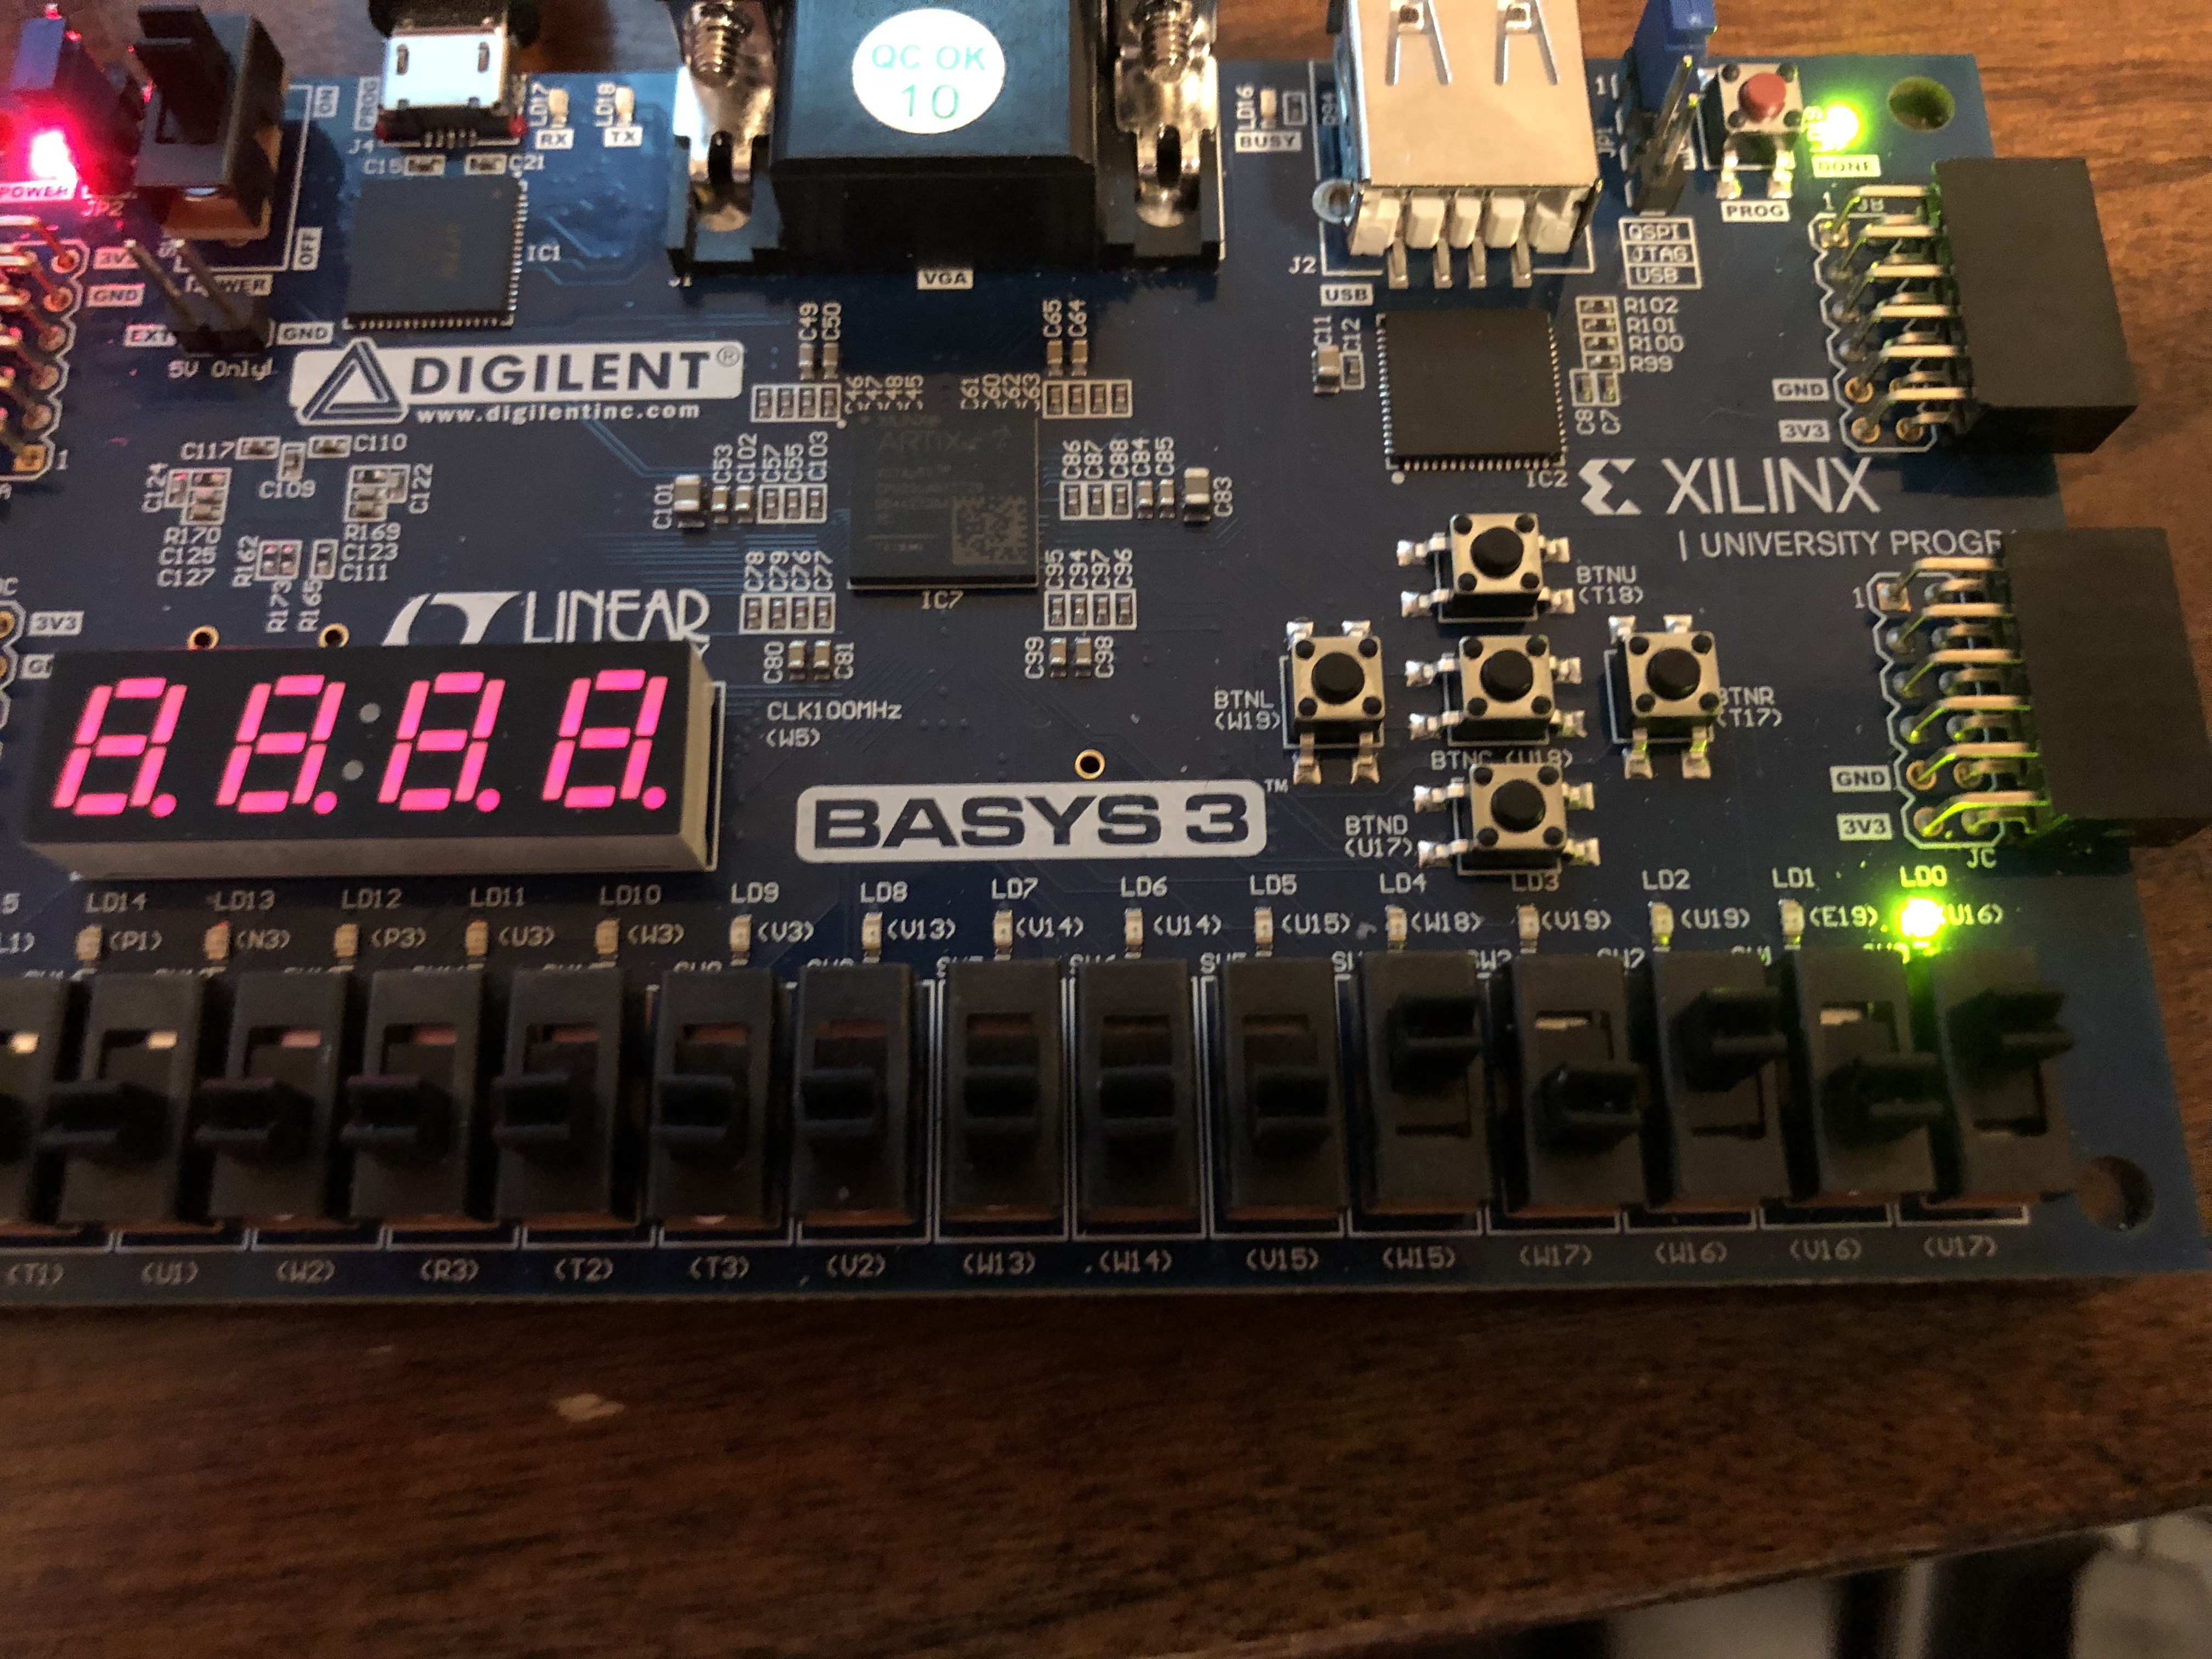
\includegraphics[width=0.5\textwidth]{./images/p1/IMG_0148.jpg}
	\caption{\label{fig:alu_res1}Operation shown: 01 OR 01 = 01}
\end{center}
\end{figure}

\begin{figure}[H]
\begin{center}
	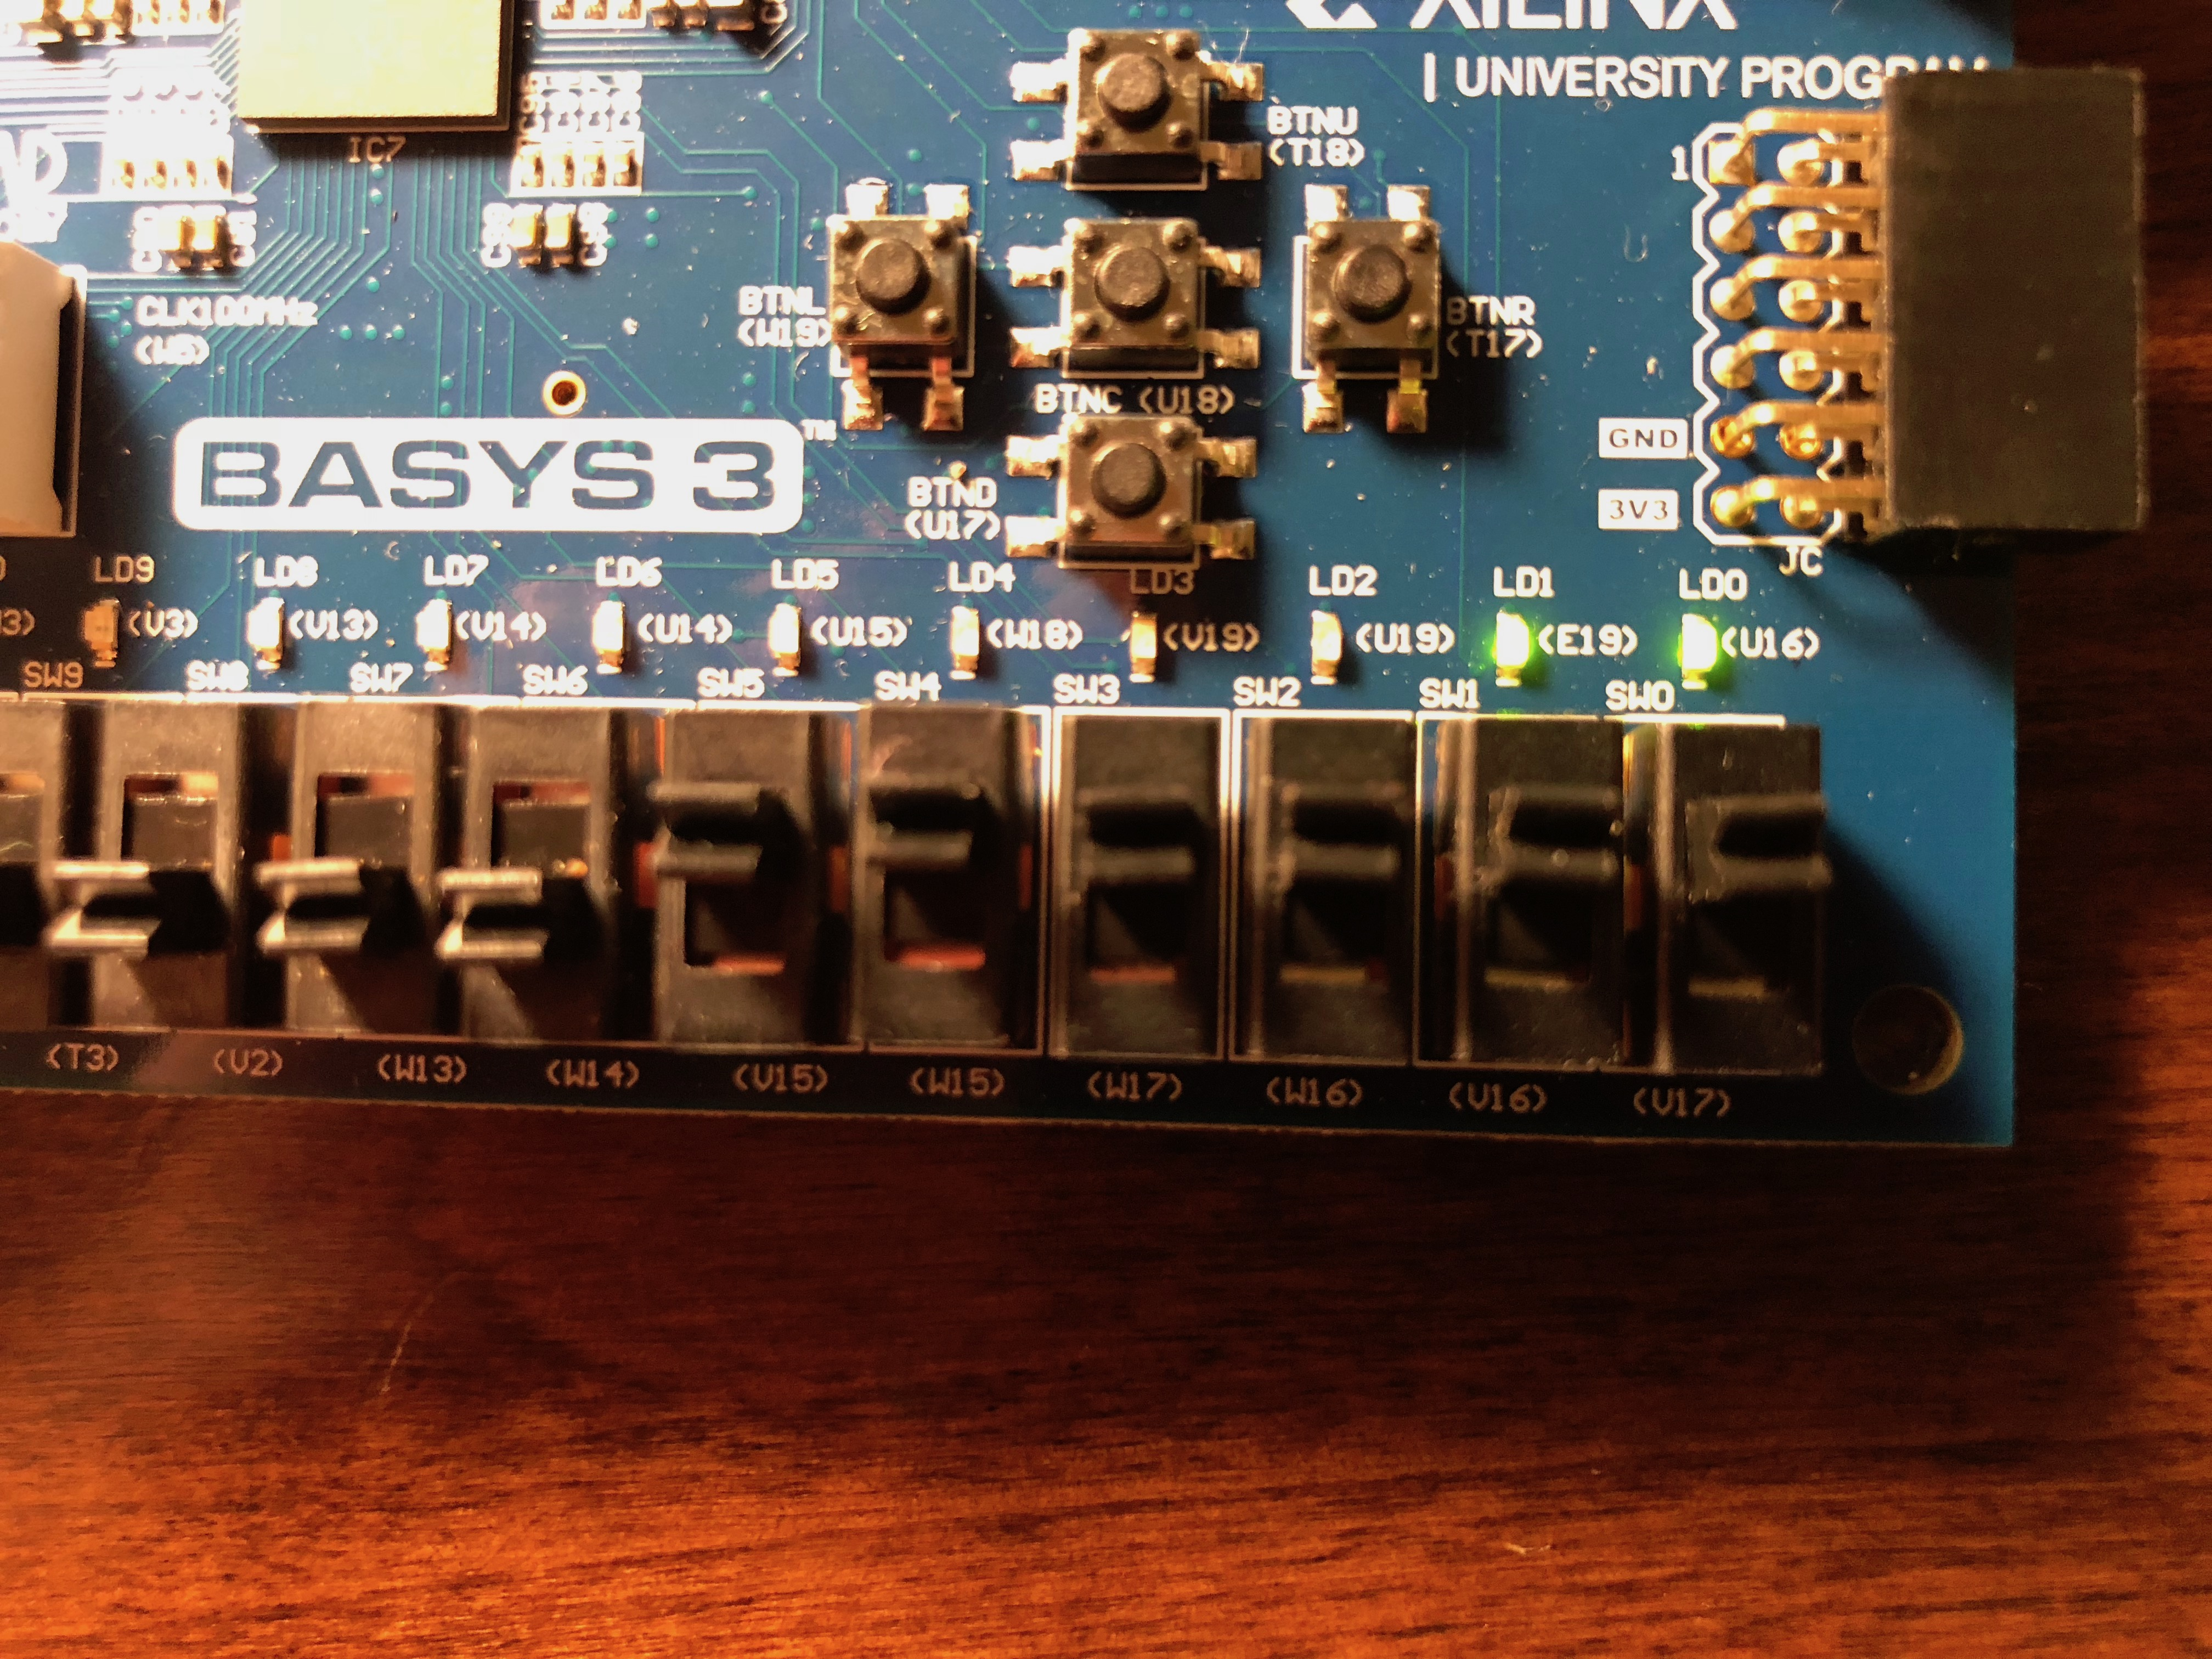
\includegraphics[width=0.5\textwidth]{./images/p1/IMG_0475.jpg}
	\caption{\label{fig:alu_res2}Operation shown: 10 OR 01 = 11}
\end{center}
\end{figure}

\begin{figure}[H]
\begin{center}
	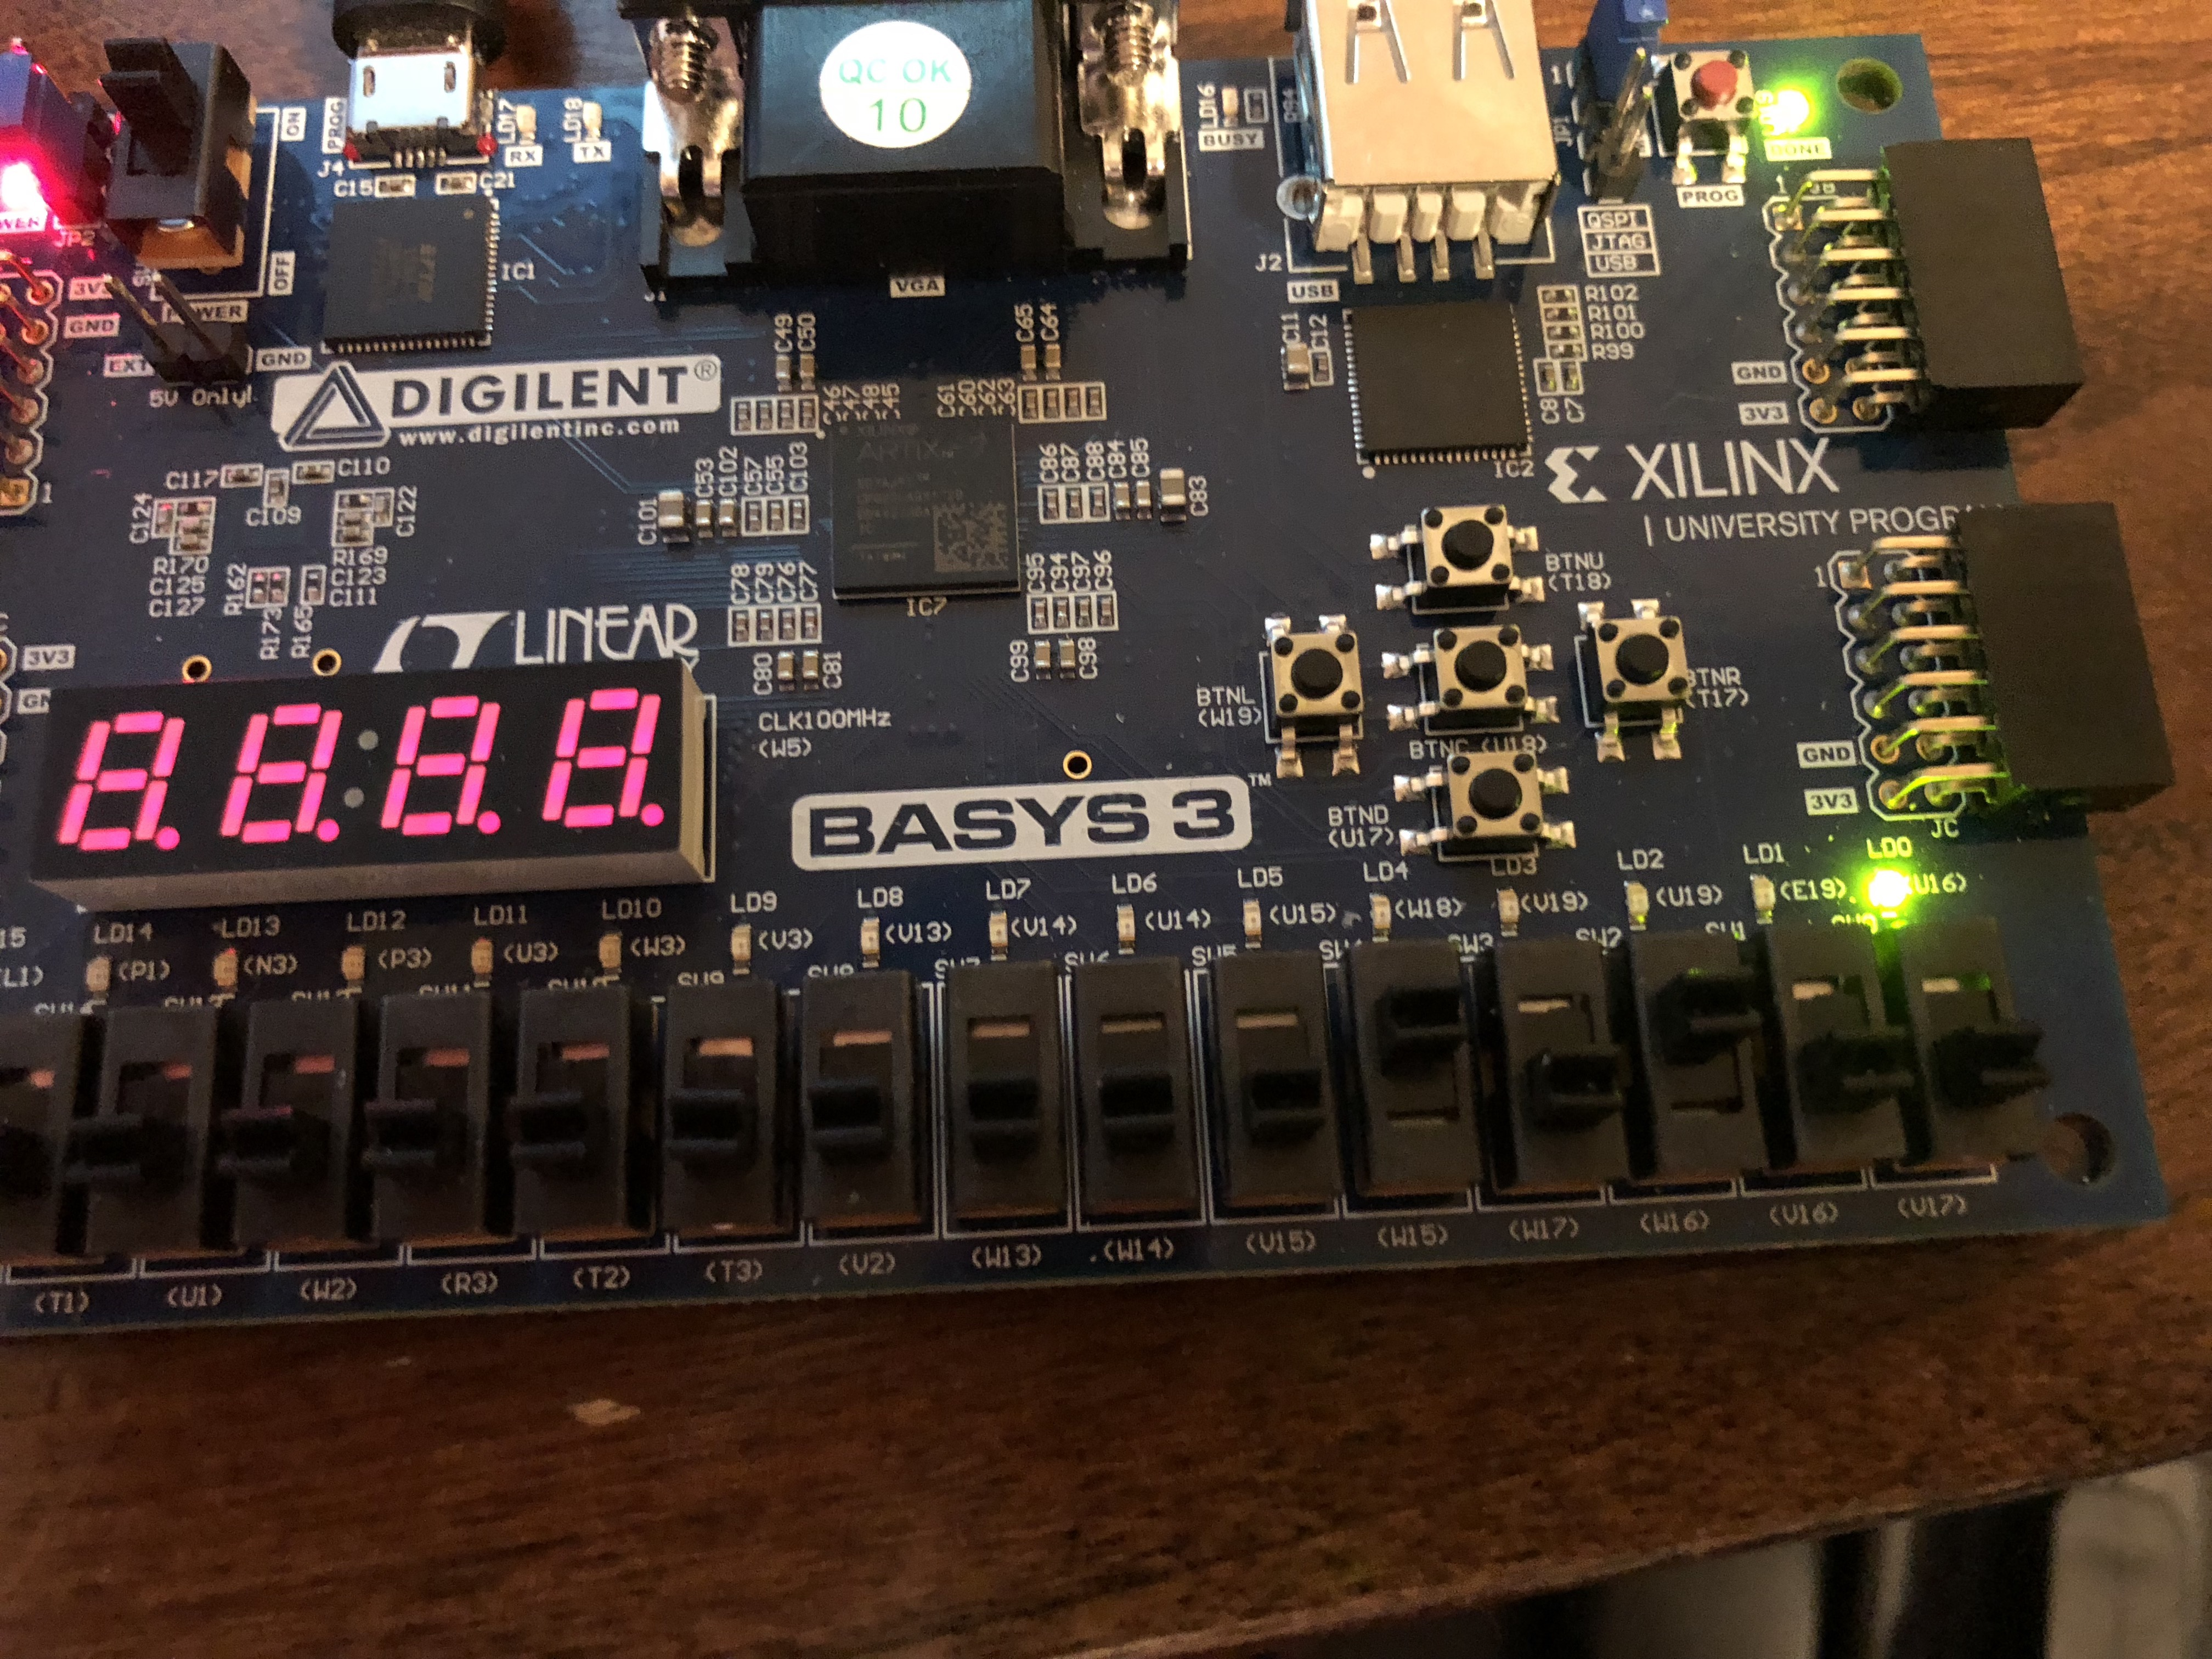
\includegraphics[width=0.5\textwidth]{./images/p1/IMG_0525.jpg}
	\caption{\label{fig:alu_res3}Operation shown: 01 OR 01 = 01}
\end{center}
\end{figure}

\begin{figure}[H]
\begin{center}
	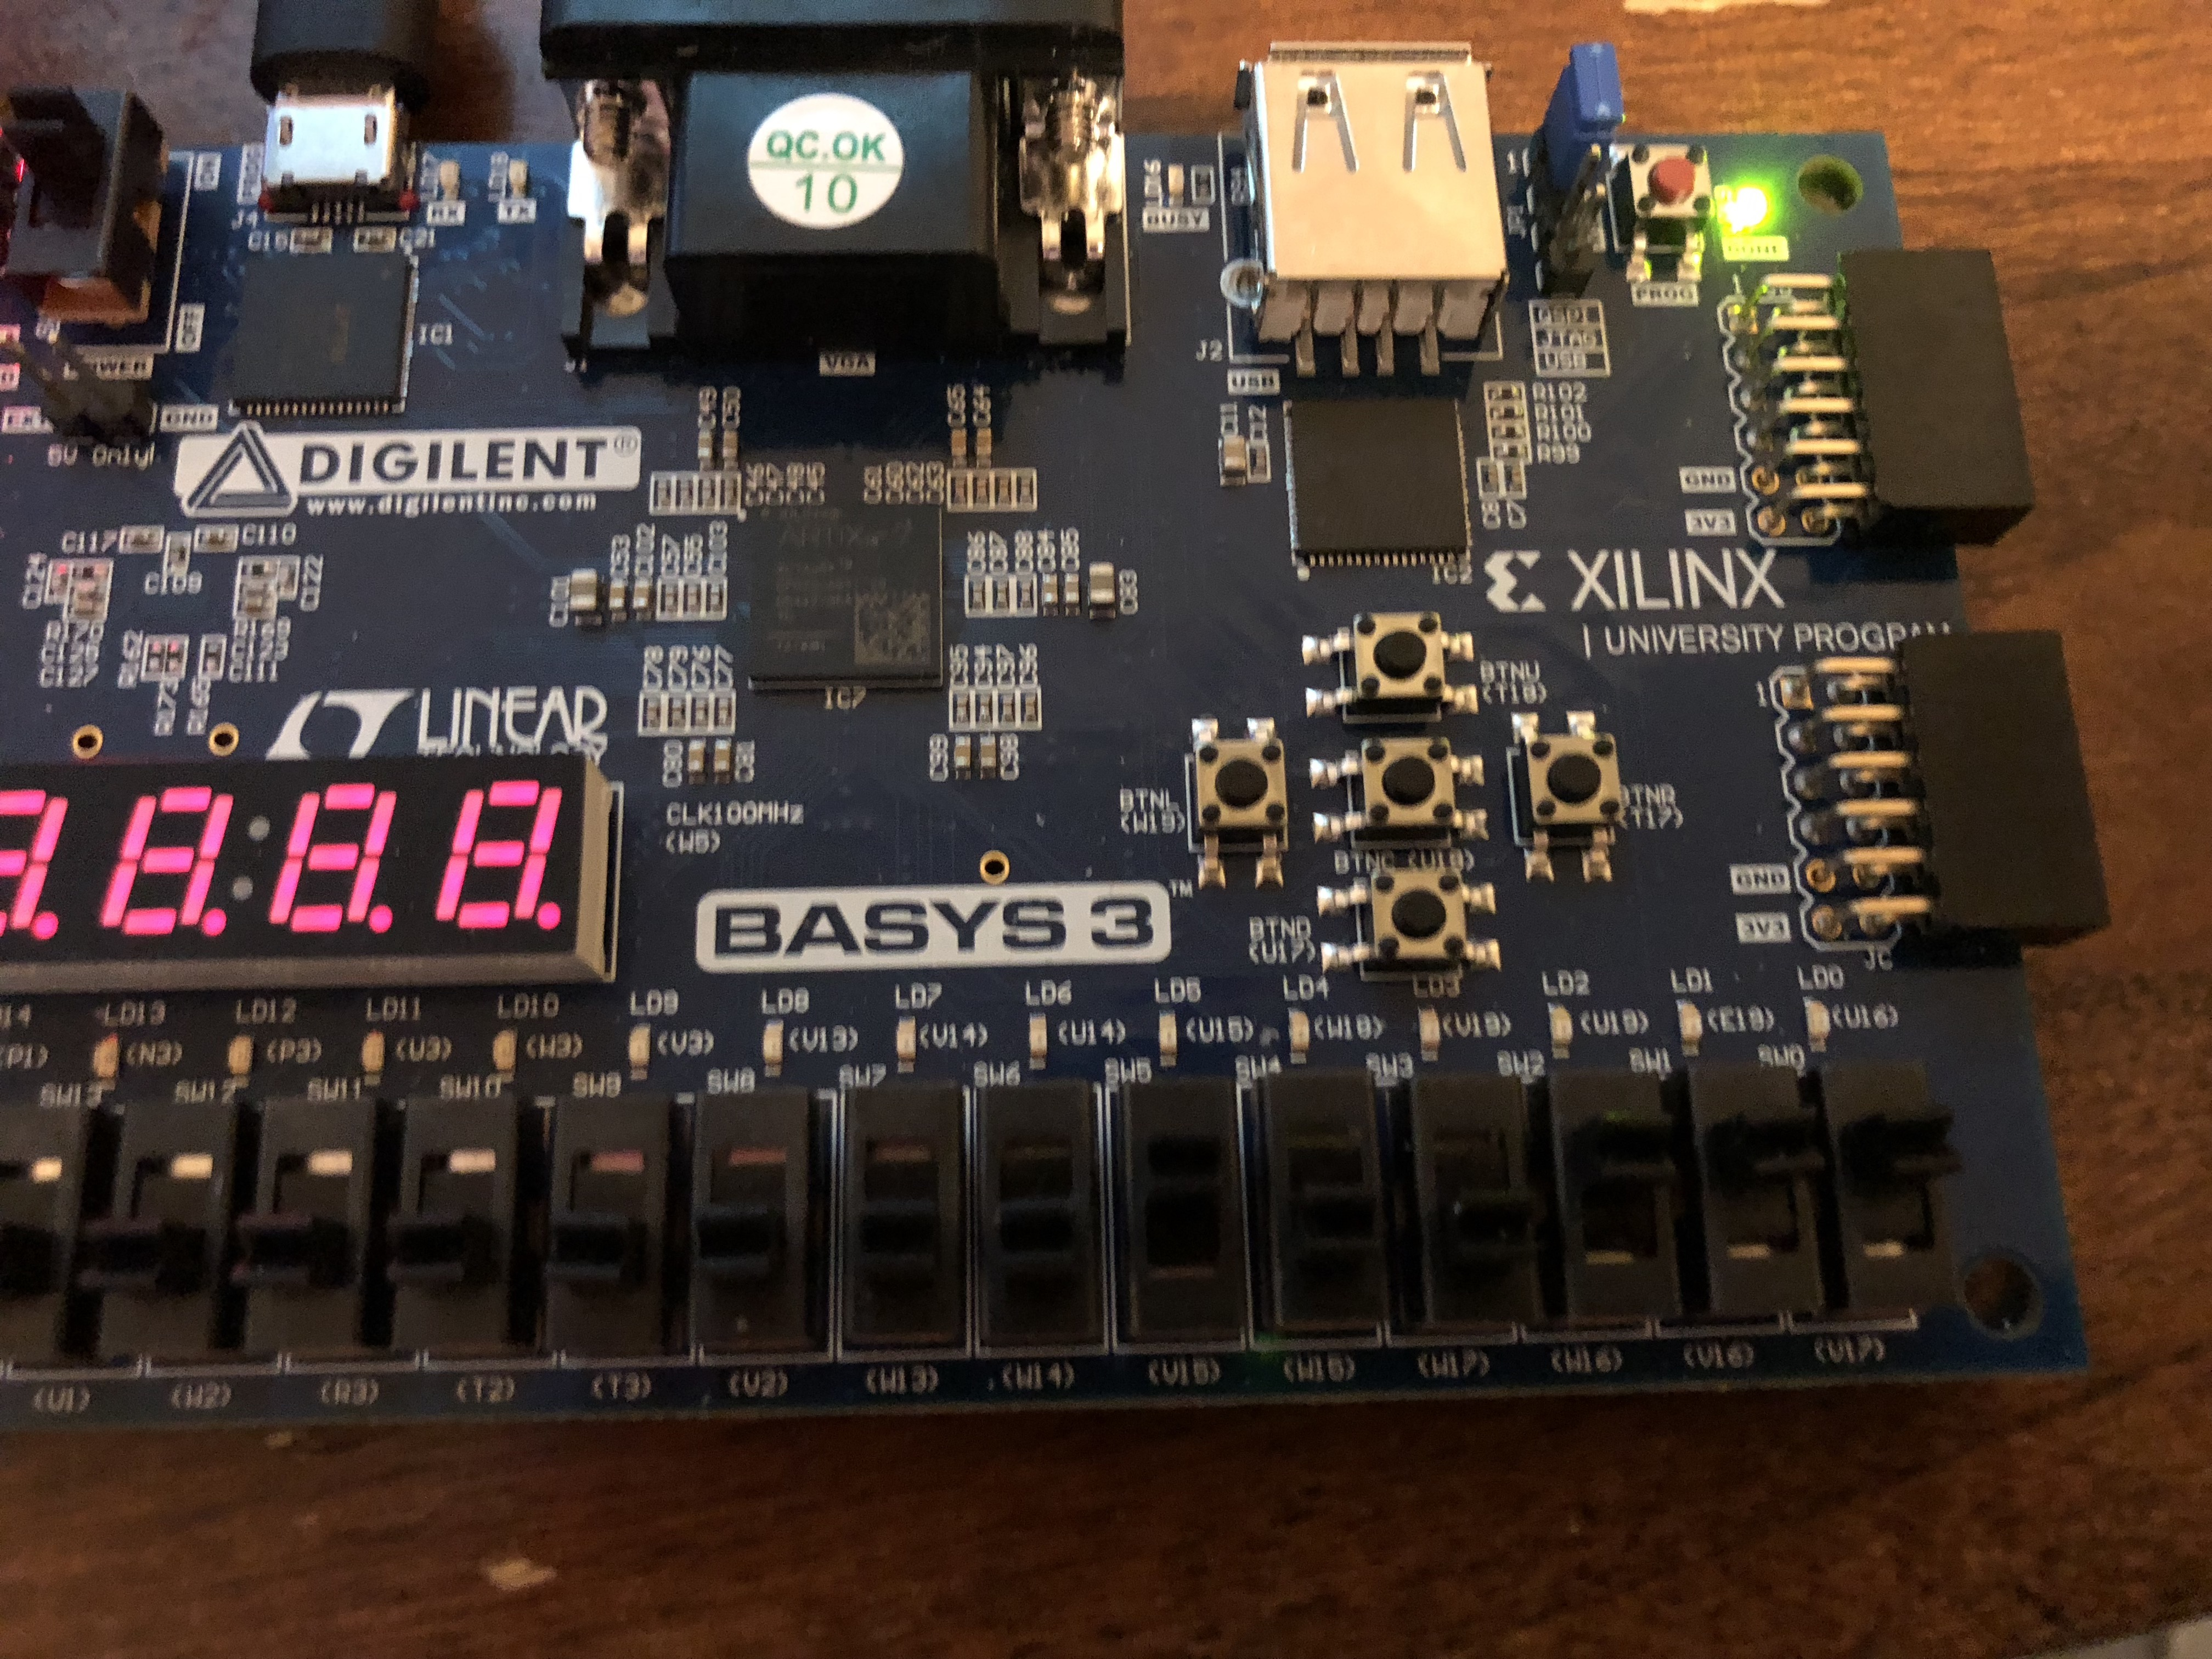
\includegraphics[width=0.5\textwidth]{./images/p1/IMG_1899.jpg}
	\caption{\label{fig:alu_res4}Operation shown: 10 Logical Shift Left by 01 = 00}
\end{center}
\end{figure}

\begin{figure}[H]
\begin{center}
	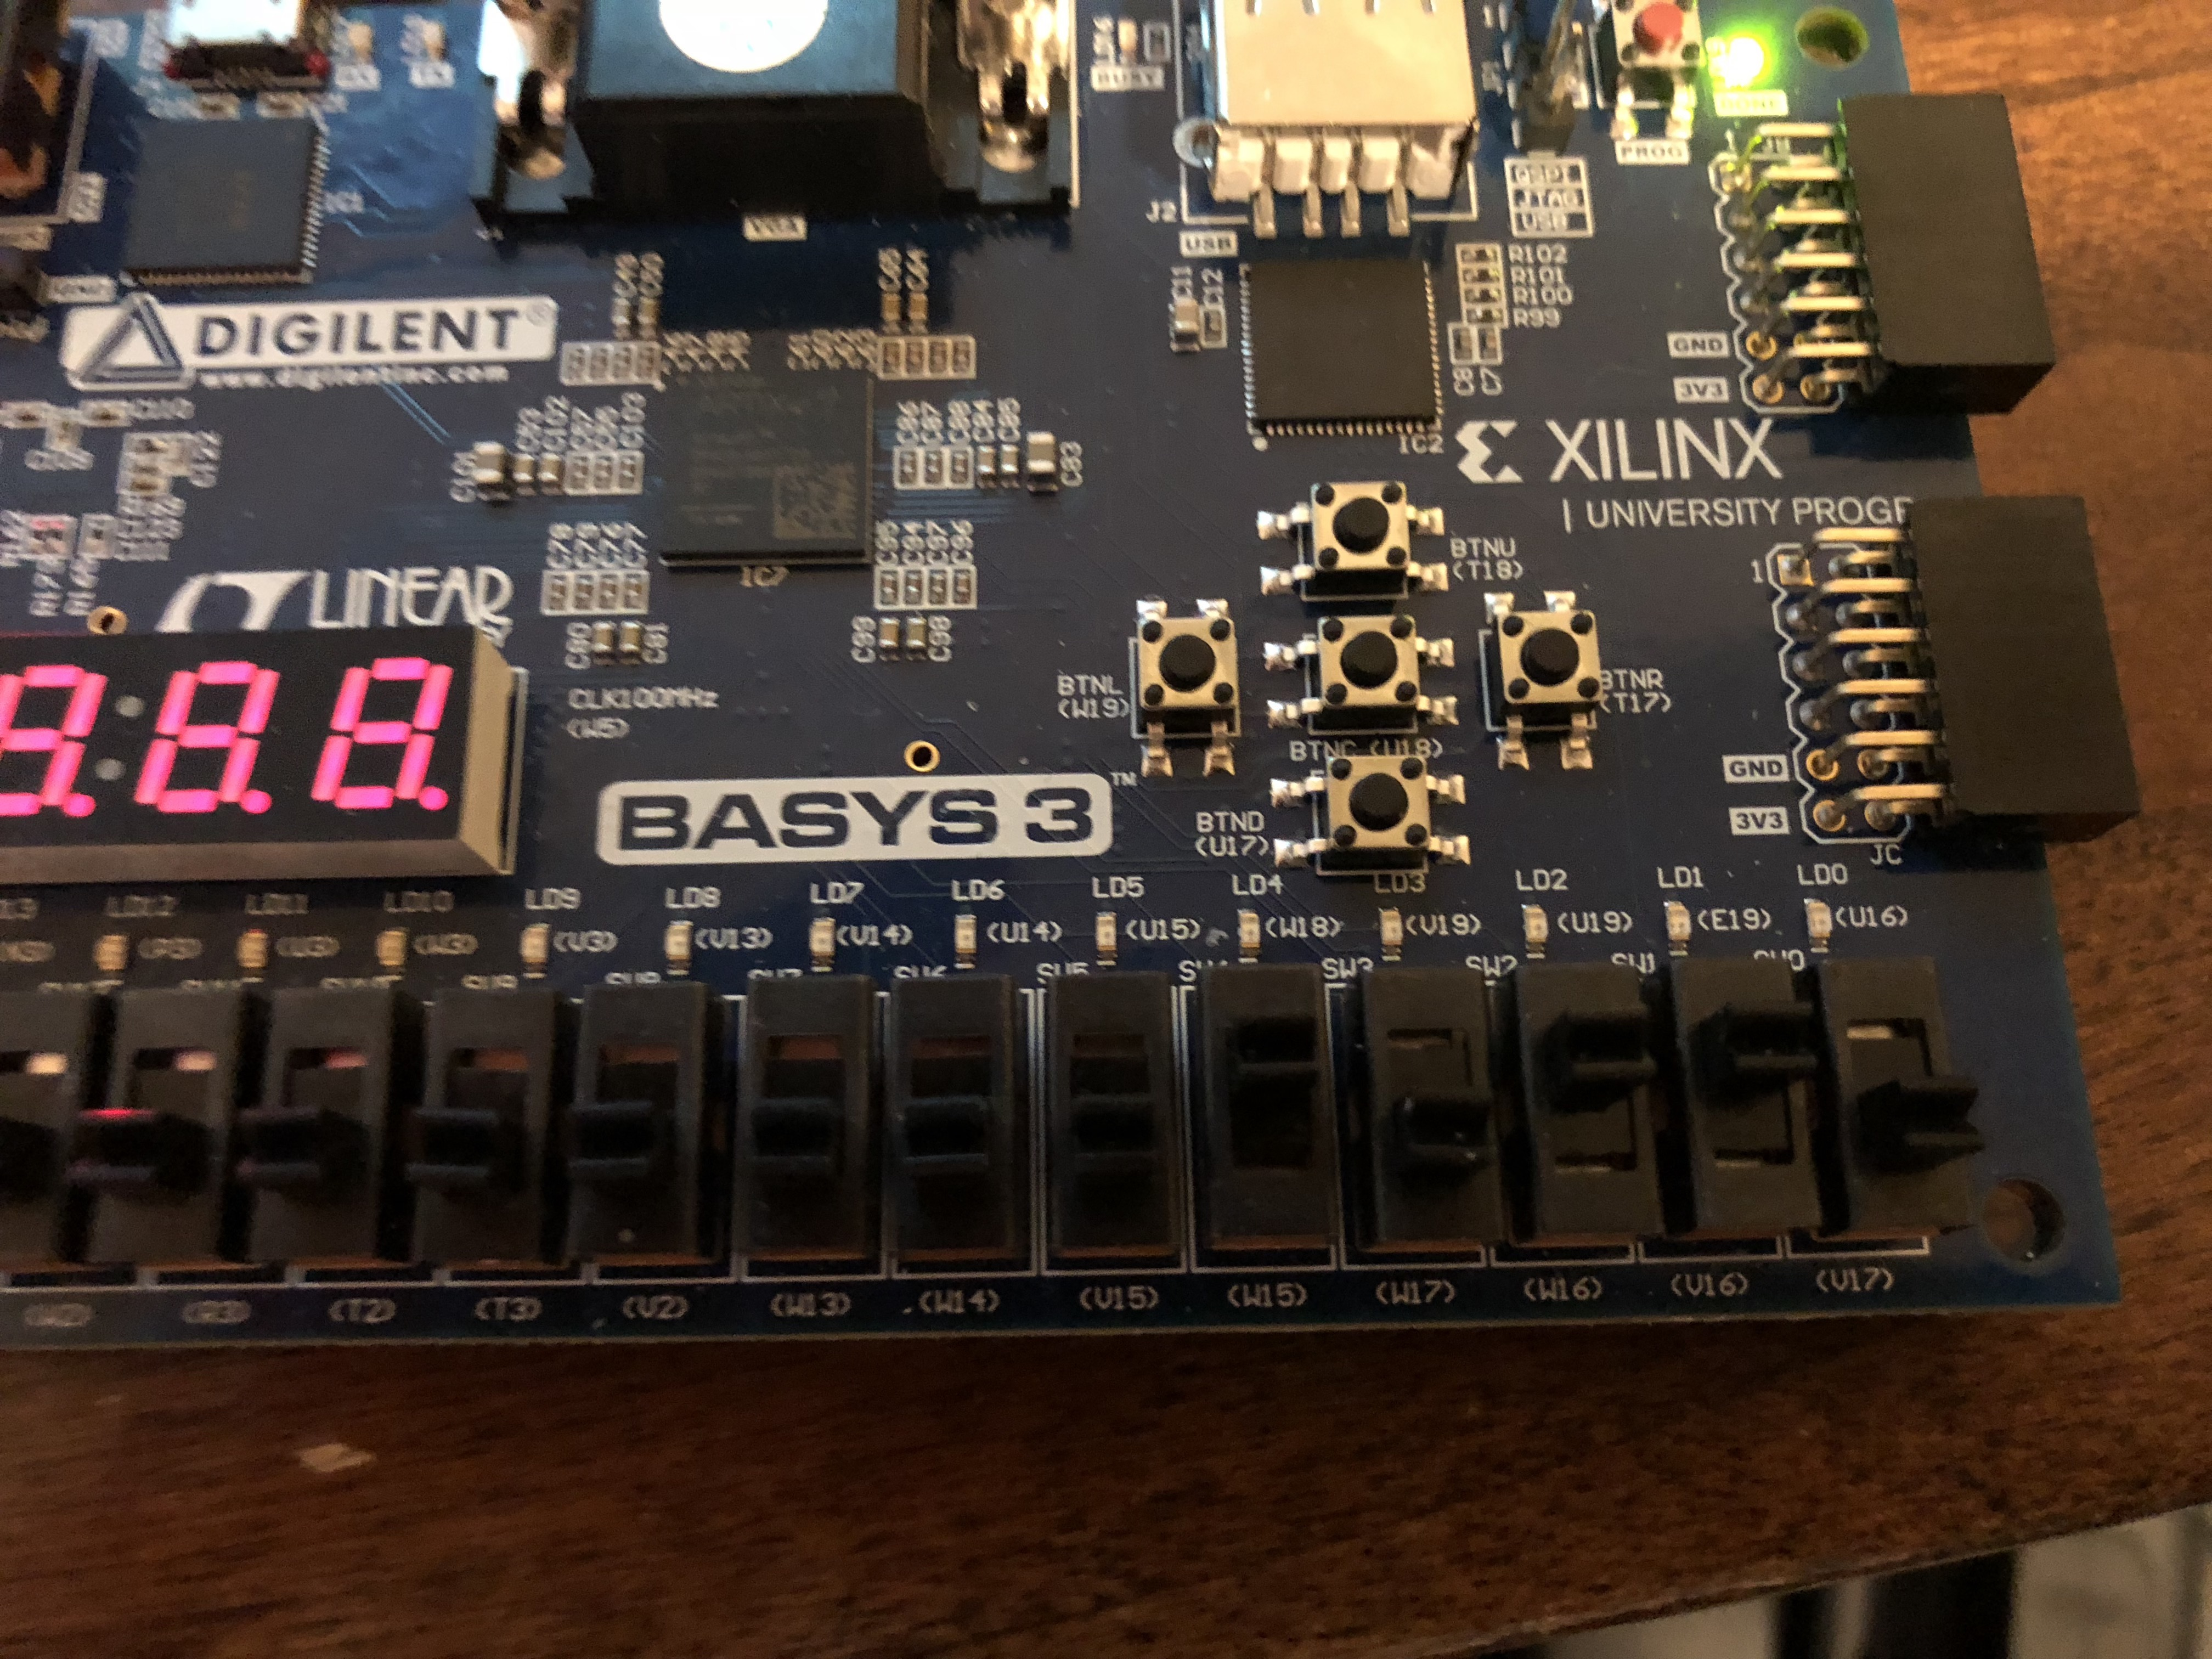
\includegraphics[width=0.5\textwidth]{./images/p1/IMG_2036.jpg}
	\caption{\label{fig:alu_res5}Operation shown: 01 Logical Shift Right by 01 = 00}
\end{center}
\end{figure}

\begin{figure}[H]
\begin{center}
	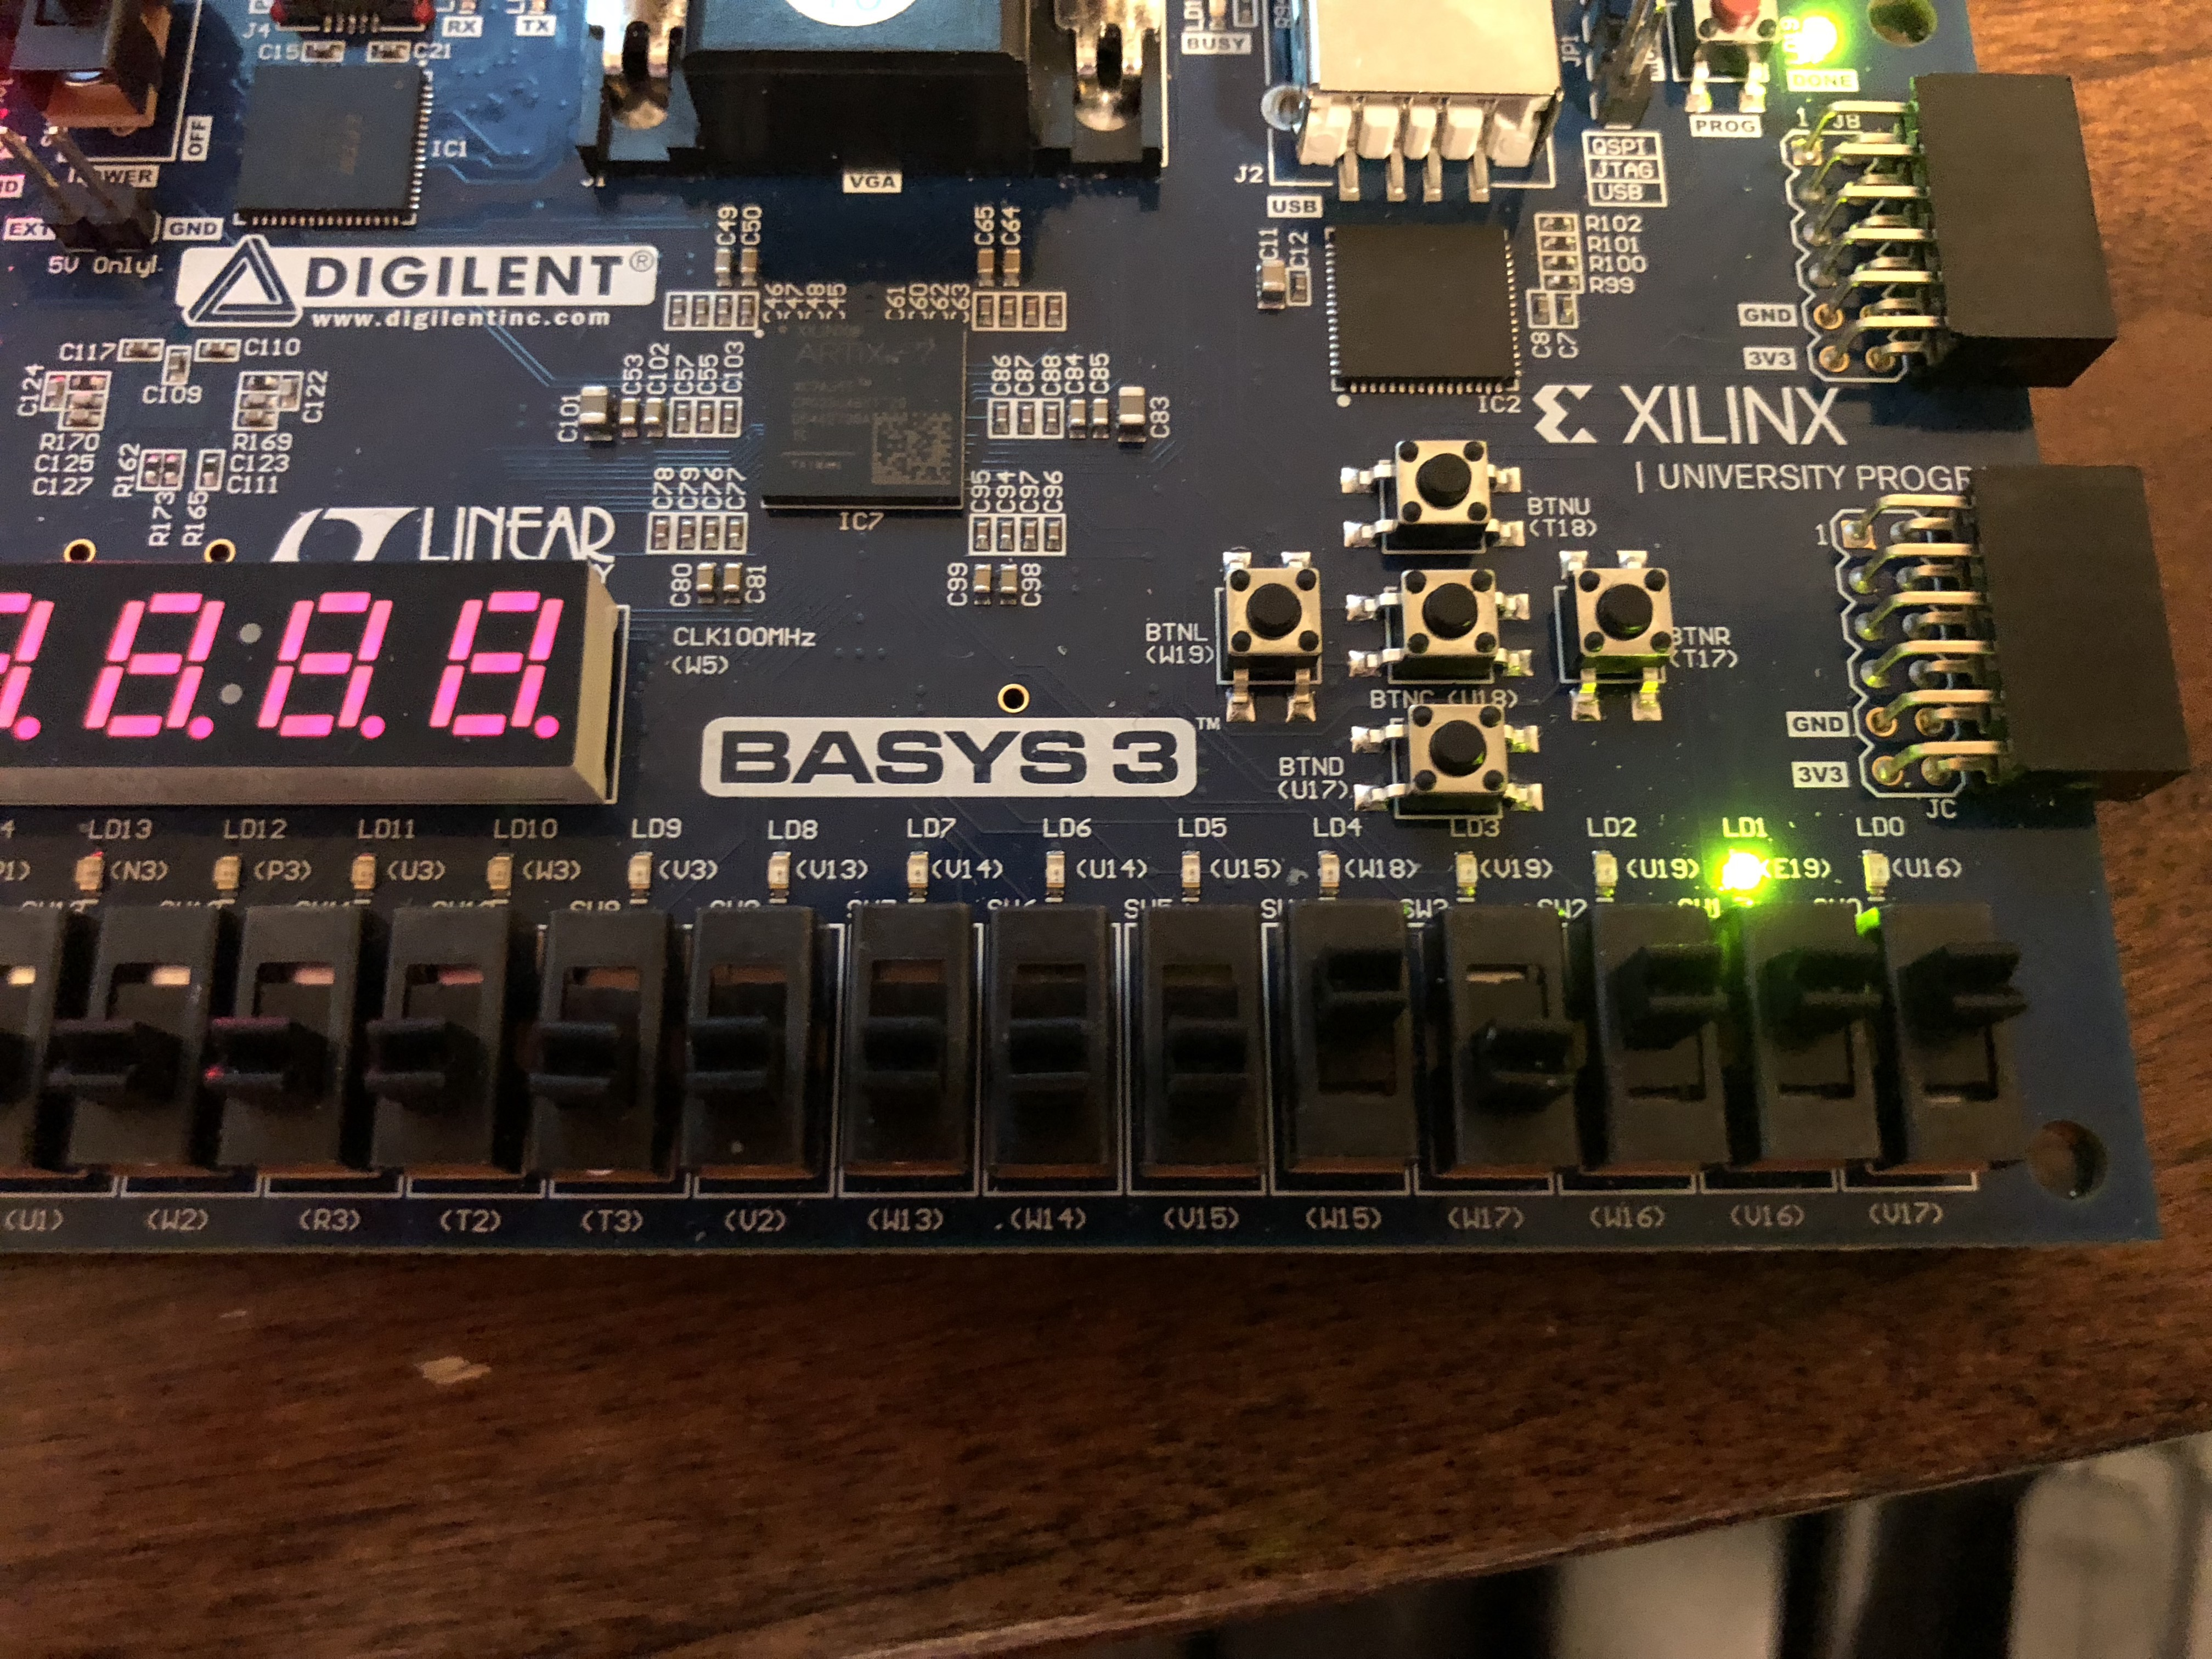
\includegraphics[width=0.5\textwidth]{./images/p1/IMG_2997.jpg}
	\caption{\label{fig:alu_res6}Operation shown: 01 Logical Shift Left by 01 = 10}
\end{center}
\end{figure}

\begin{figure}[H]
\begin{center}
	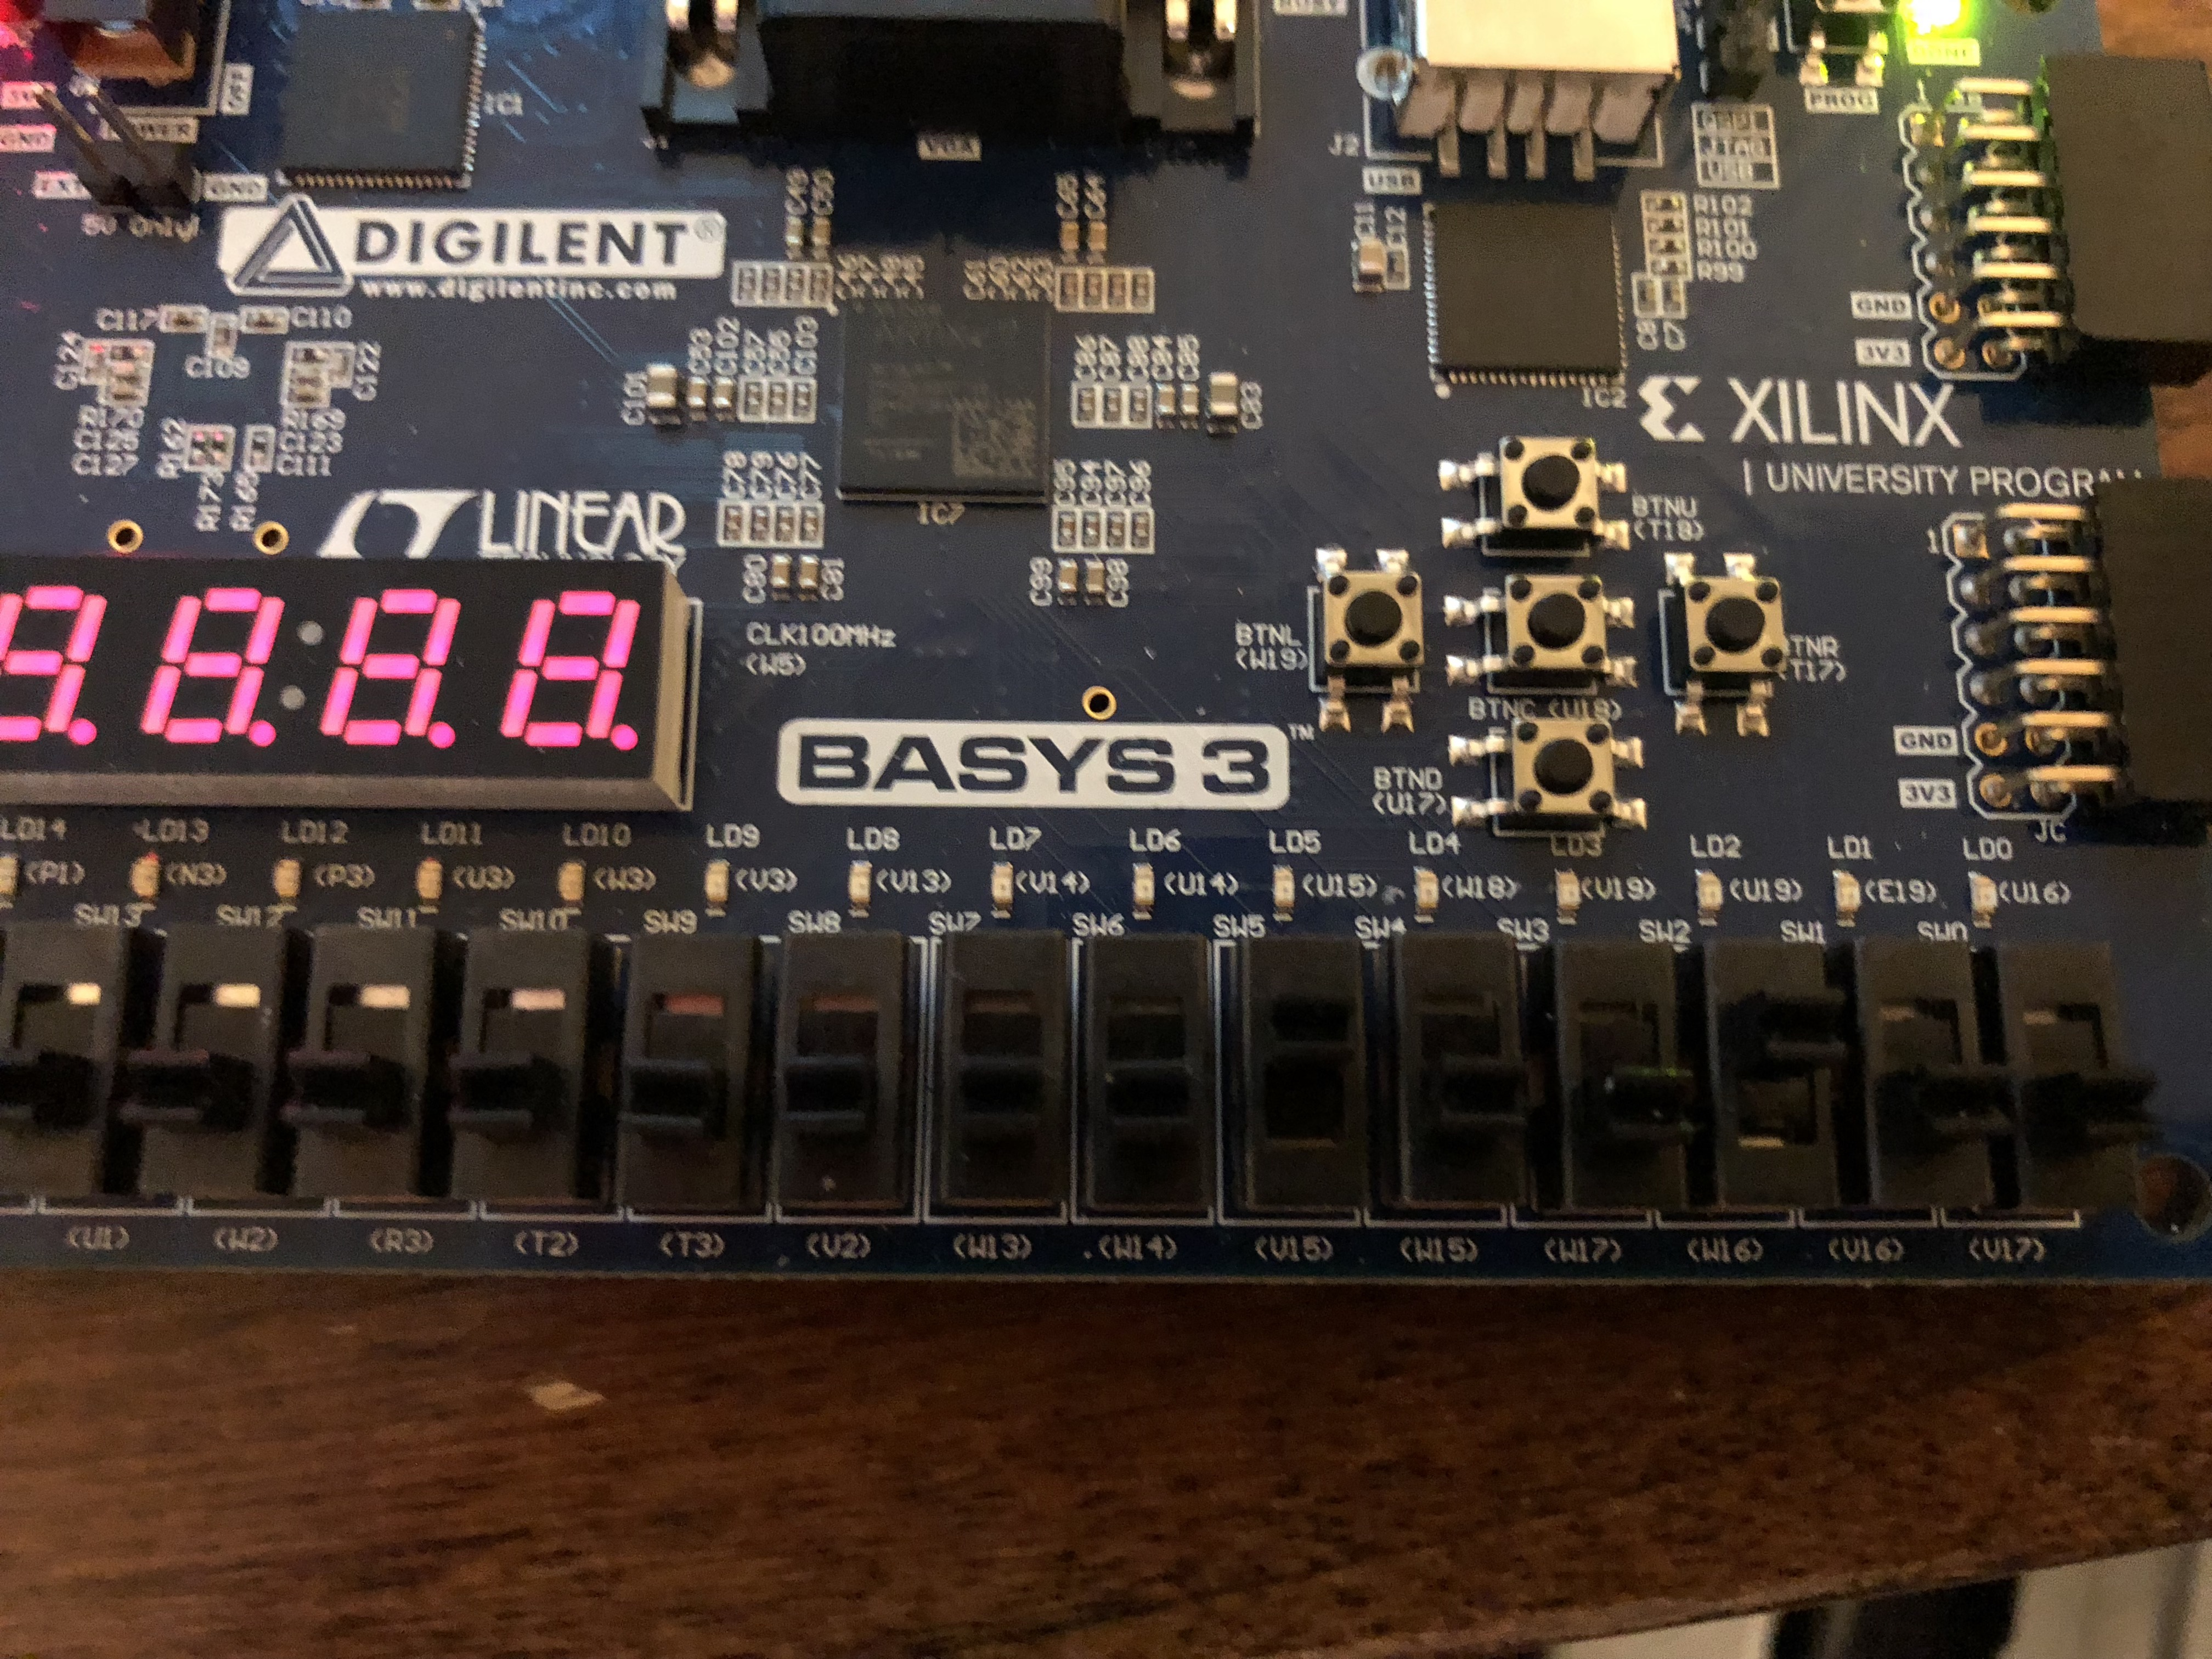
\includegraphics[width=0.5\textwidth]{./images/p1/IMG_5830.jpg}
	\caption{\label{fig:alu_res7}Operation shown: 10 AND 01 = 00}
\end{center}
\end{figure}

\begin{figure}[H]
\begin{center}
	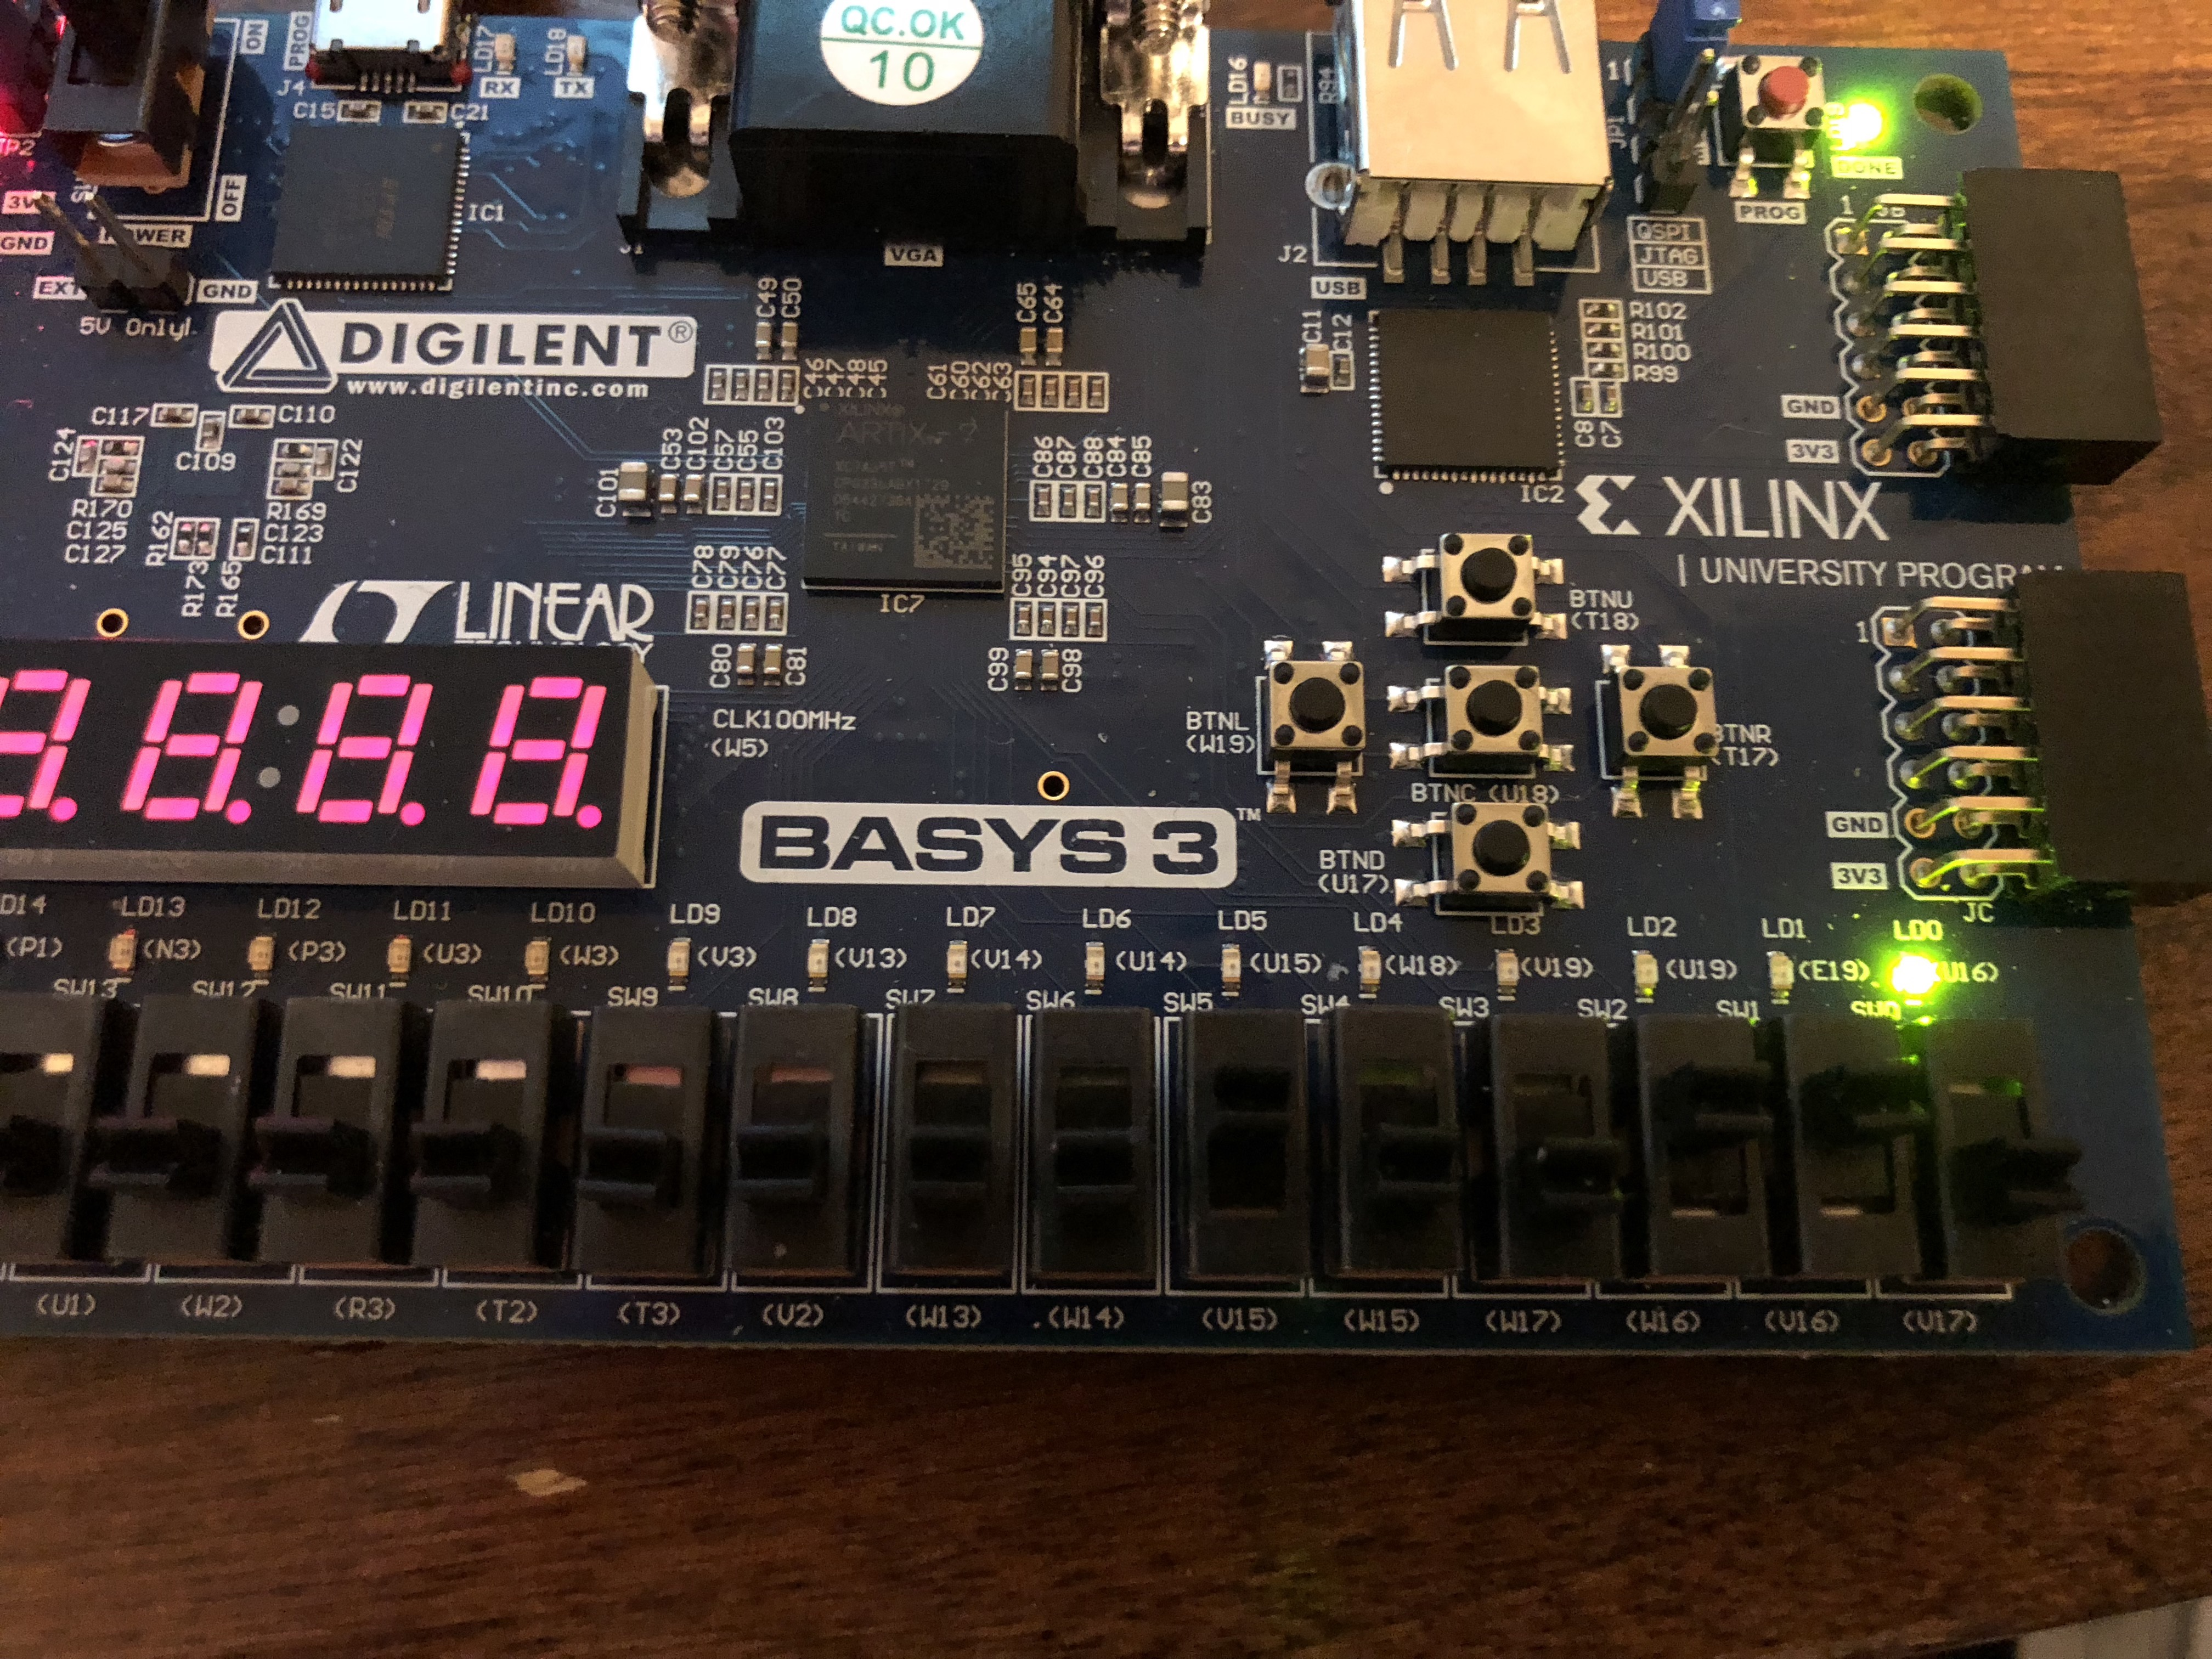
\includegraphics[width=0.5\textwidth]{./images/p1/IMG_7938.jpg}
	\caption{\label{fig:alu_res8}Operation shown: 10 Logical Shift Right by 01 = 01}
\end{center}
\end{figure}

\subsection{Problem 2 }

\subsubsection{Background}
For problem 2, we are instructed to create a simple Finite State Machine that will issue the four different commands needed to operate the arithmetic logic unit created in Problem 1.

\subsubsection{Design Solution}
Because there are four possible commands, and our select input from Problem 1 has 2-bits, we know that this state machine requires 2 bits and four possible states. We also utilized our clock divider from a previous lab to slow down the clock signal we are using the allow this machine to be tested and observed on the Basys3. The input and output ports for this design are shown in Tables ~\ref{tab:fsm_input_Ports} and ~\ref{tab:fsm_output_Ports}, respectively. The state diagram is displayed in Figure ~\ref{fig:fsm_state_diagram}.

\begin{table}[H]
\begin{center}
\begin{tabular}{| l | l | l |}
	\hline
	Bit & Label & Port \\ \hline
	clk &  Clock & W5 \\ \hline
	enable & Switch 0 & V17 \\ \hline
	reset & Button Right & T17 \\ \hline
\end{tabular}
\caption{\label{tab:fsm_input_Ports}Input port assignments for  the finite state machine.}
\end{center}
\end{table}

\begin{table}[H]
\begin{center}
\begin{tabular}{| l | l | l |}
	\hline
	Bit & Label & Port \\ \hline
	output\_sel[0] & LED 0 & U16 \\ \hline
	output\_sel[1] & LED 1 & E19 \\ \hline
\end{tabular}
\caption{\label{tab:fsm_output_Ports}Output port assignments for the finite state machine.}
\end{center}
\end{table}

\begin{center}
\begin{figure}[H]
	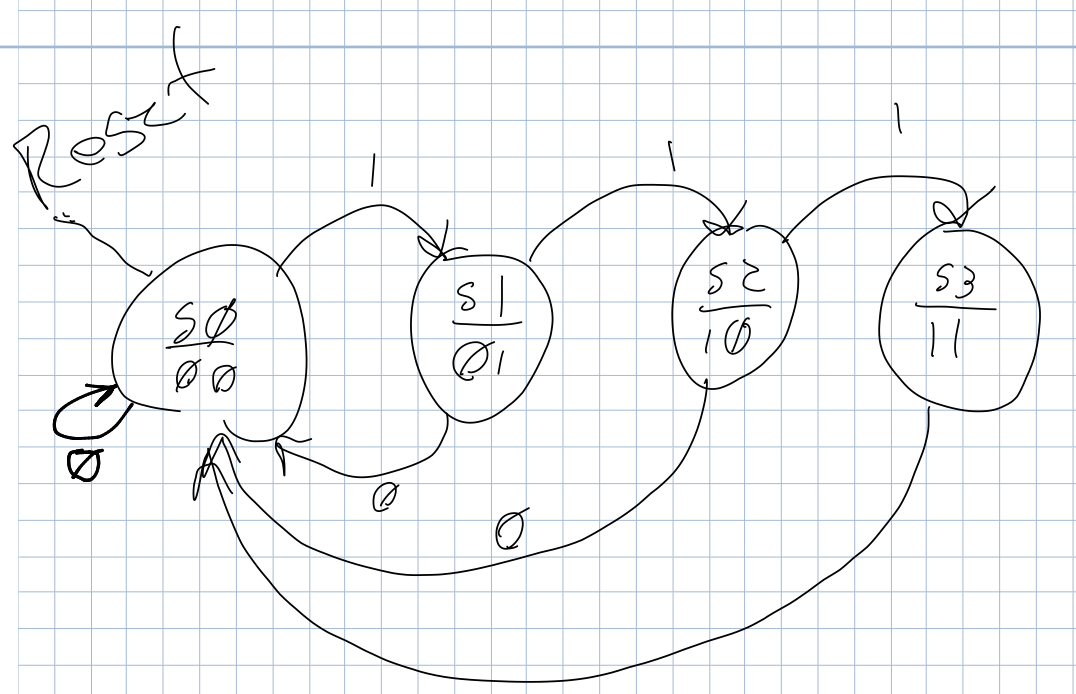
\includegraphics[width=\textwidth]{./images/fsmStateDiagram.png}
	\caption{\label{fig:fsm_state_diagram}State diagram based off of the "enable" input.}
\end{figure}
\end{center}

\subsubsection{Results}

\begin{figure}[H]
\begin{center}
	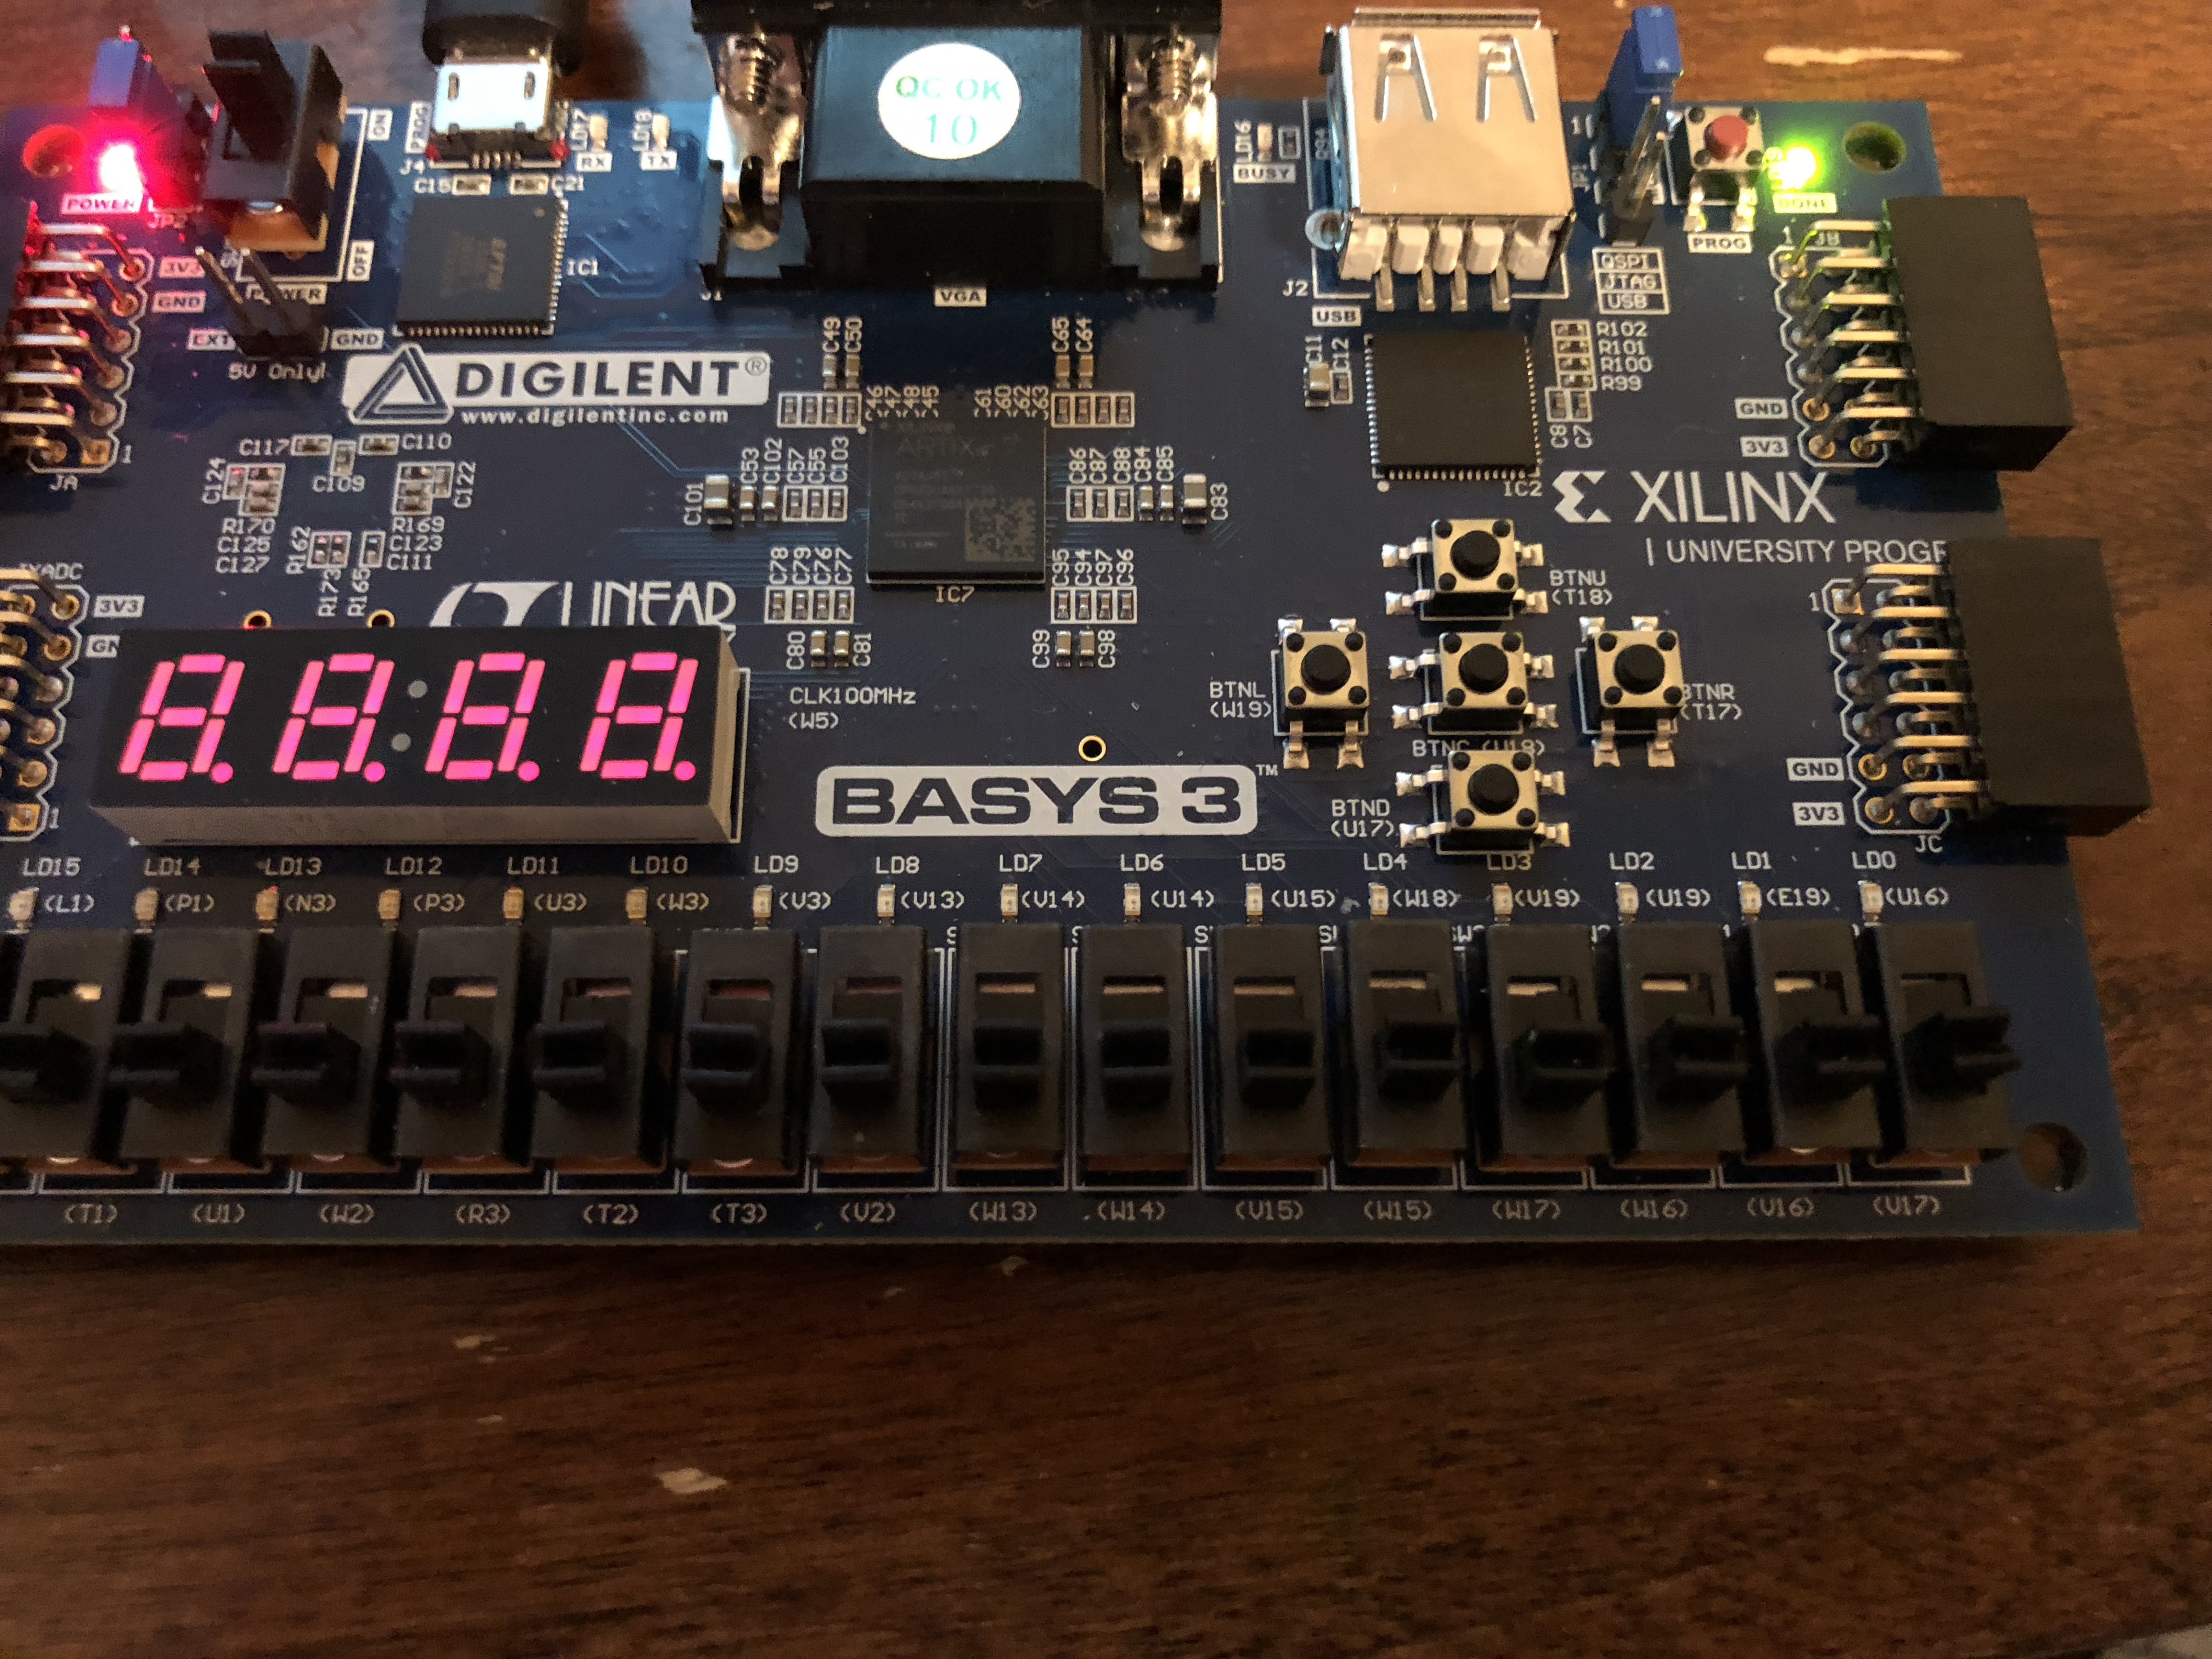
\includegraphics[width=0.5\textwidth]{./images/p2/IMG_2172.jpg}
	\caption{\label{fig:fsm_res1}Finite state machine is staying in state 0 while receiving input 0.}
\end{center}
\end{figure}

\begin{figure}[H]
\begin{center}
	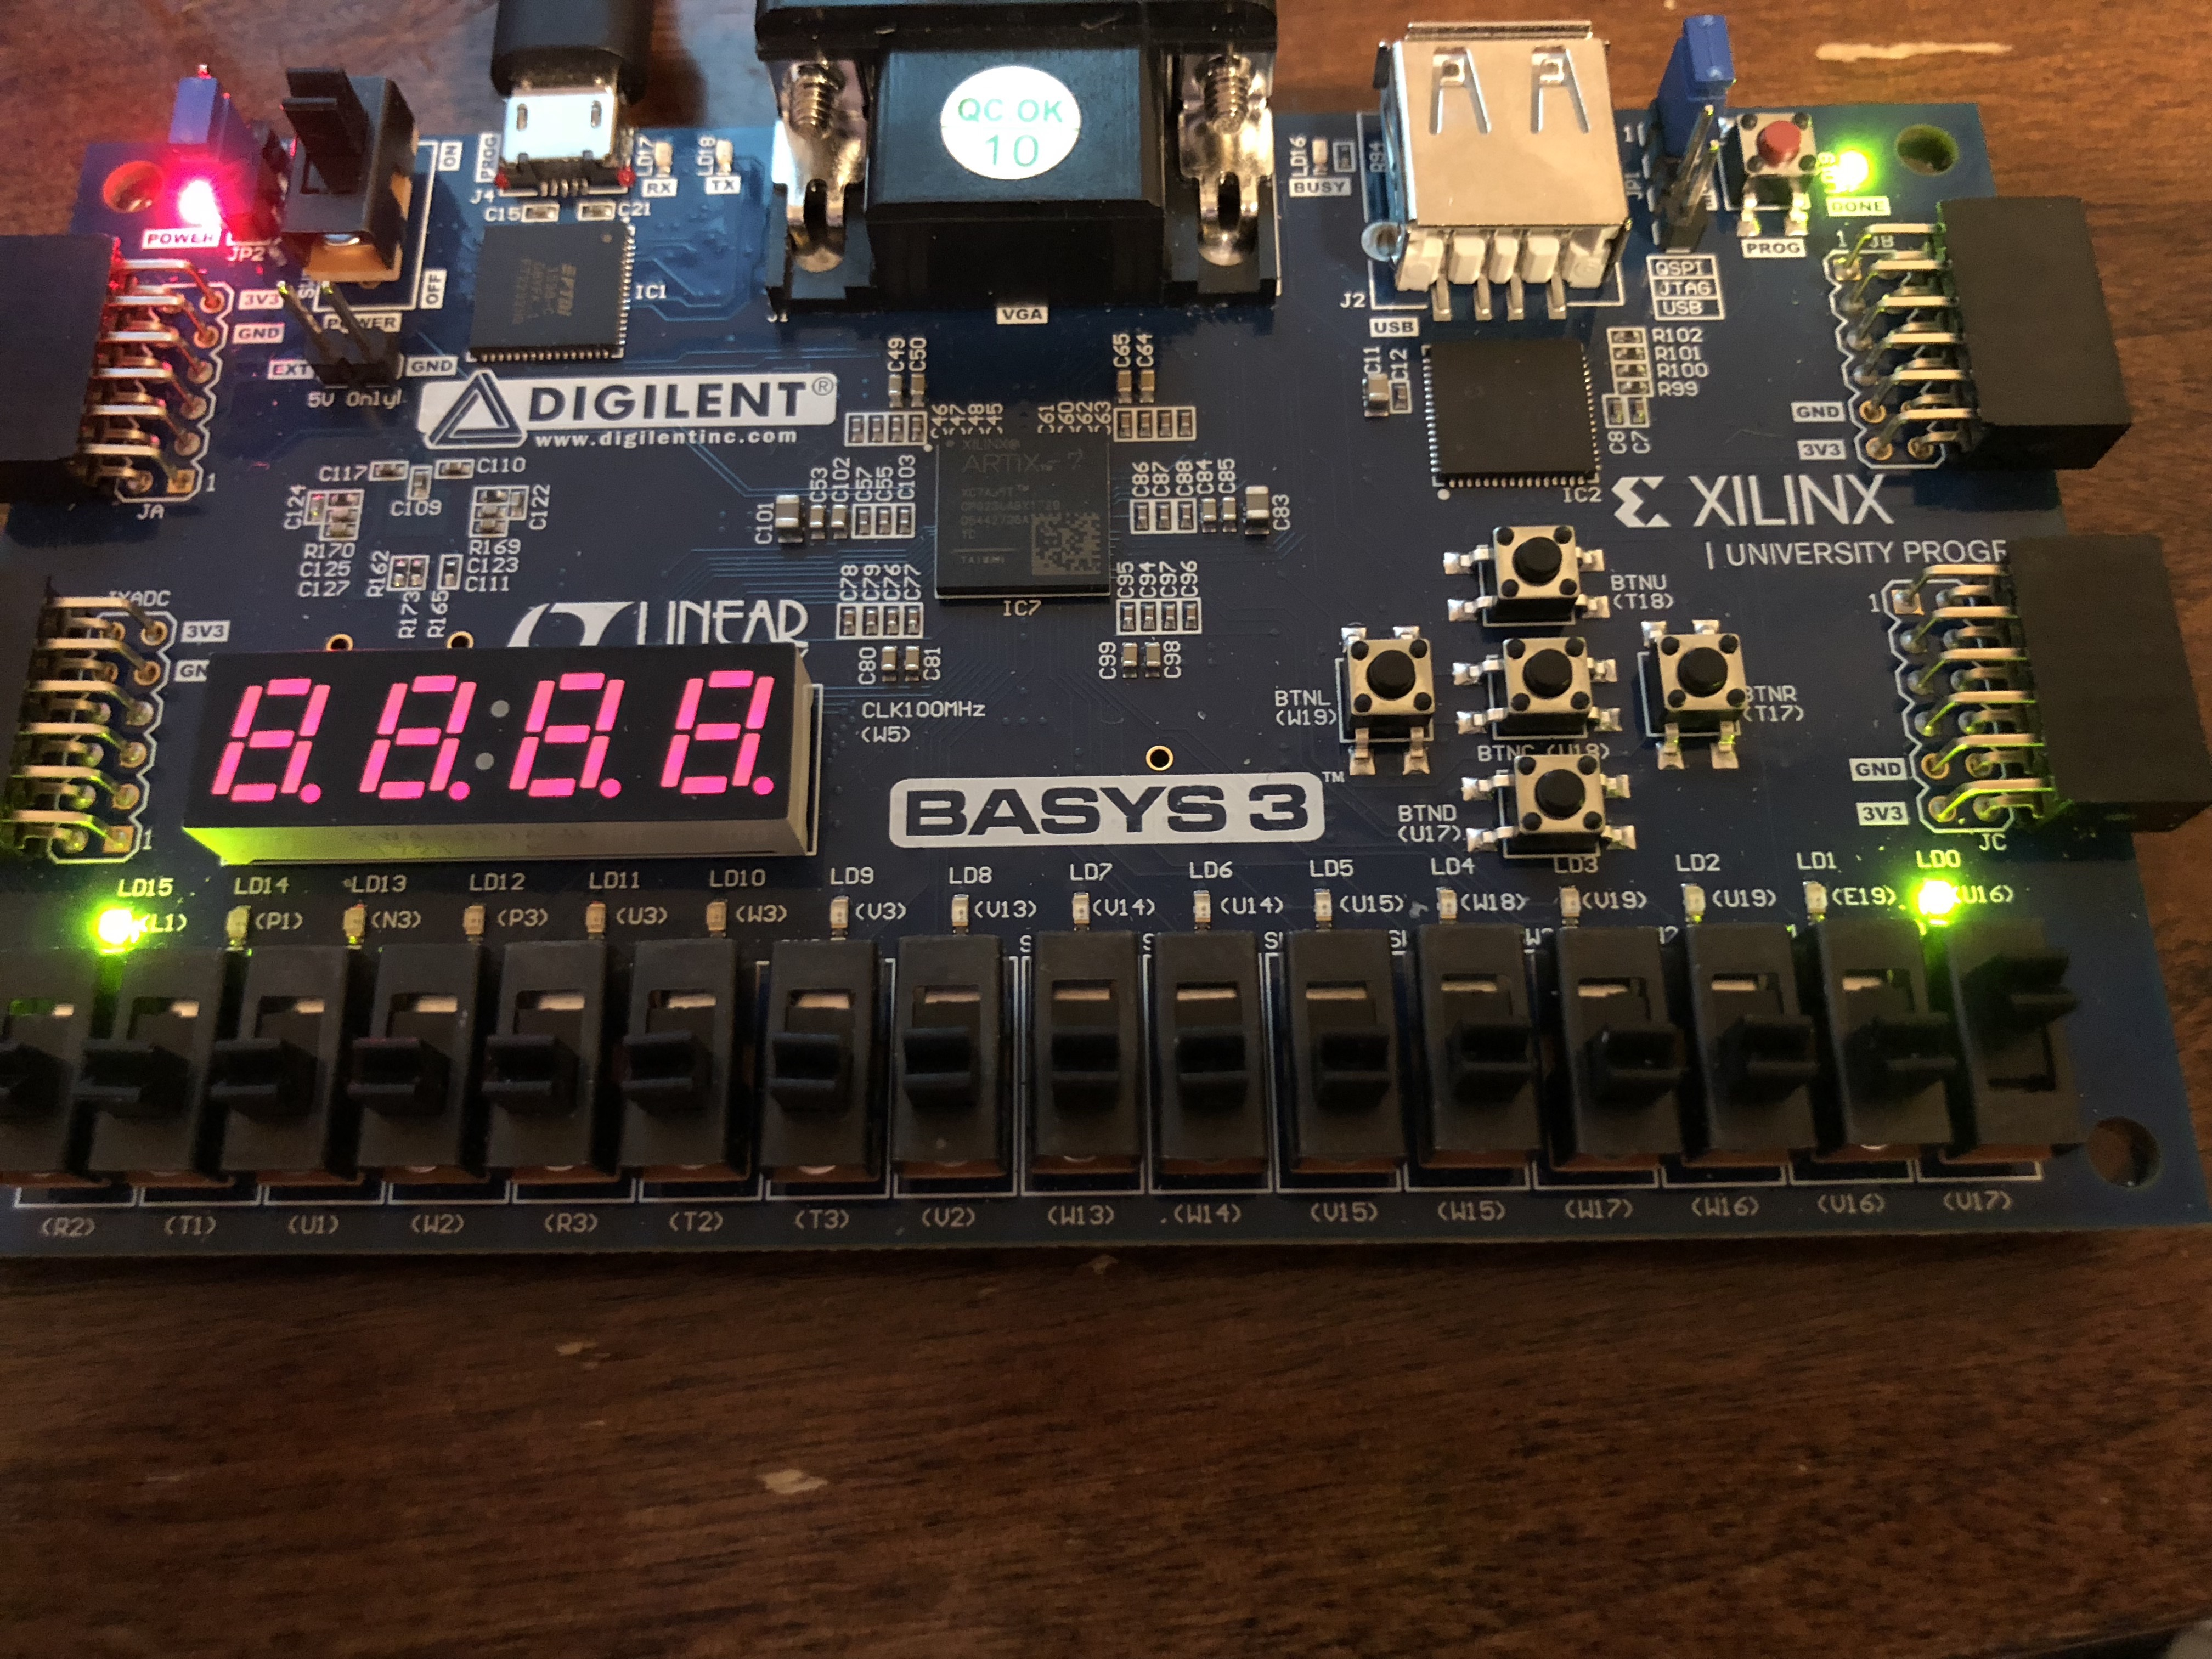
\includegraphics[width=0.5\textwidth]{./images/p2/IMG_9245.jpg}
	\caption{\label{fig:fsm_res2}FSM is in state 1.}
\end{center}
\end{figure}

\begin{figure}[H]
\begin{center}
	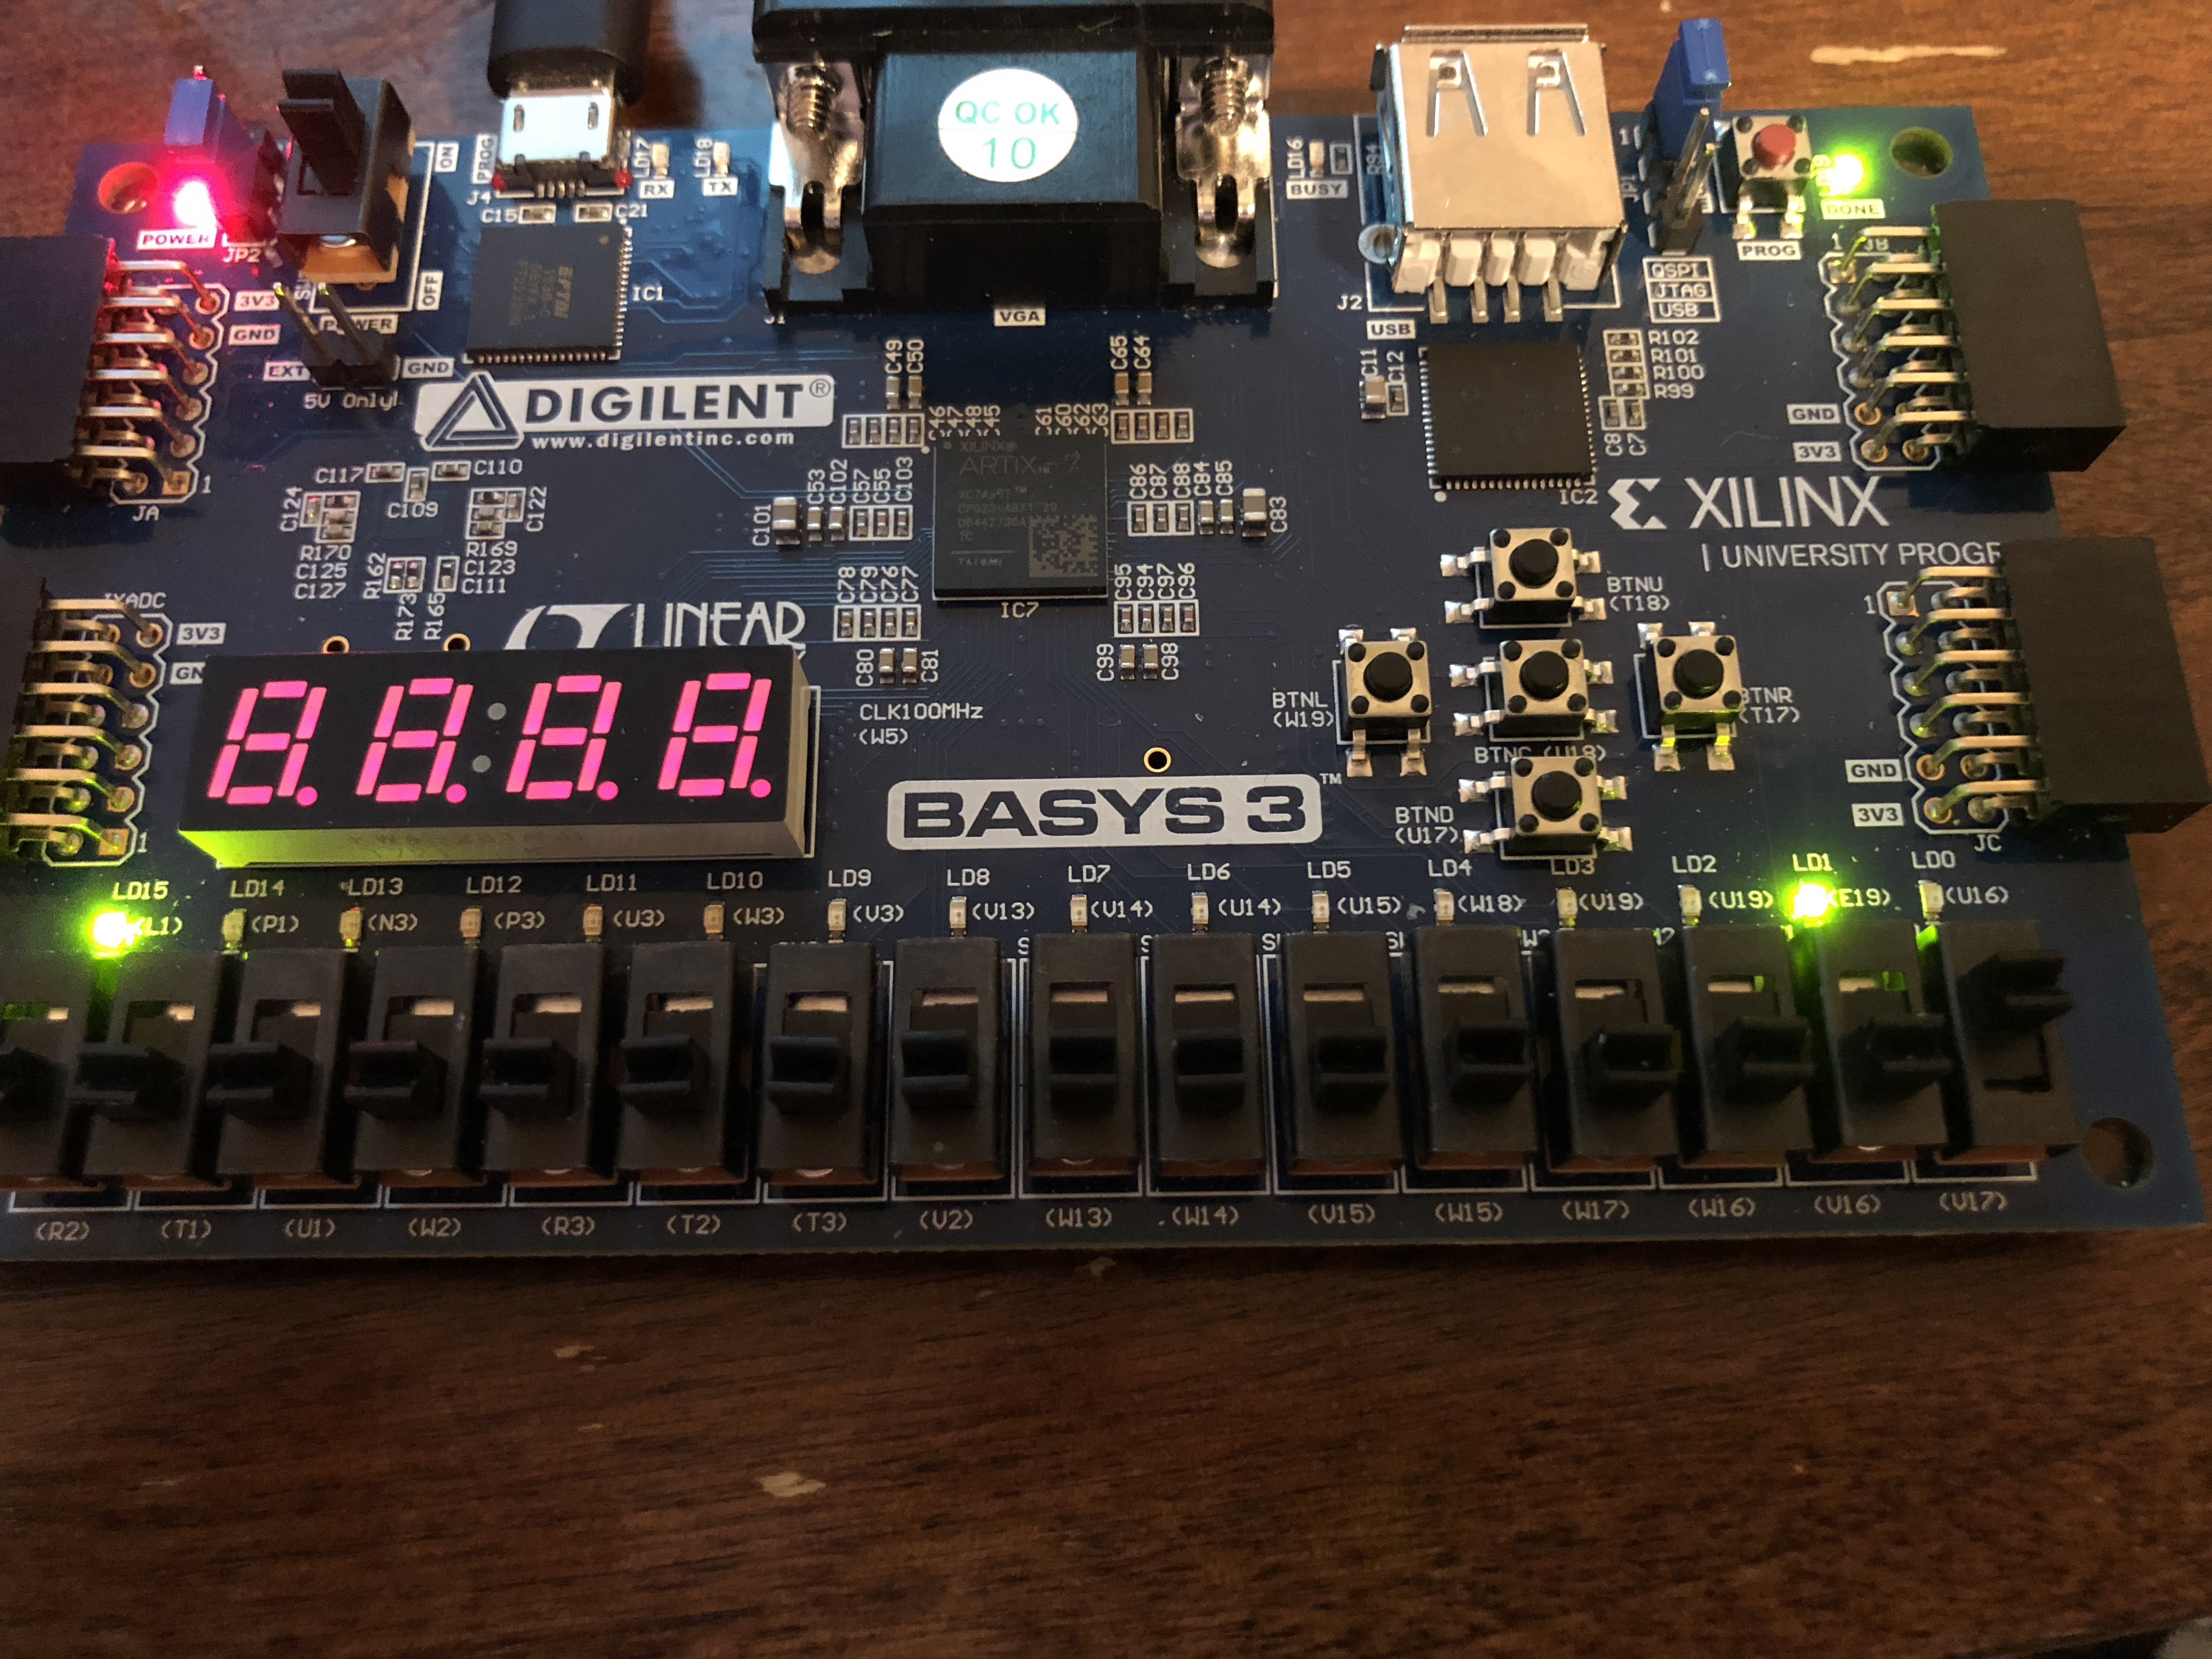
\includegraphics[width=0.5\textwidth]{./images/p2/IMG_1509.jpg}
	\caption{\label{fig:fsm_res3}FSM is in state 2.}
\end{center}
\end{figure}

\begin{figure}[H]
\begin{center}
	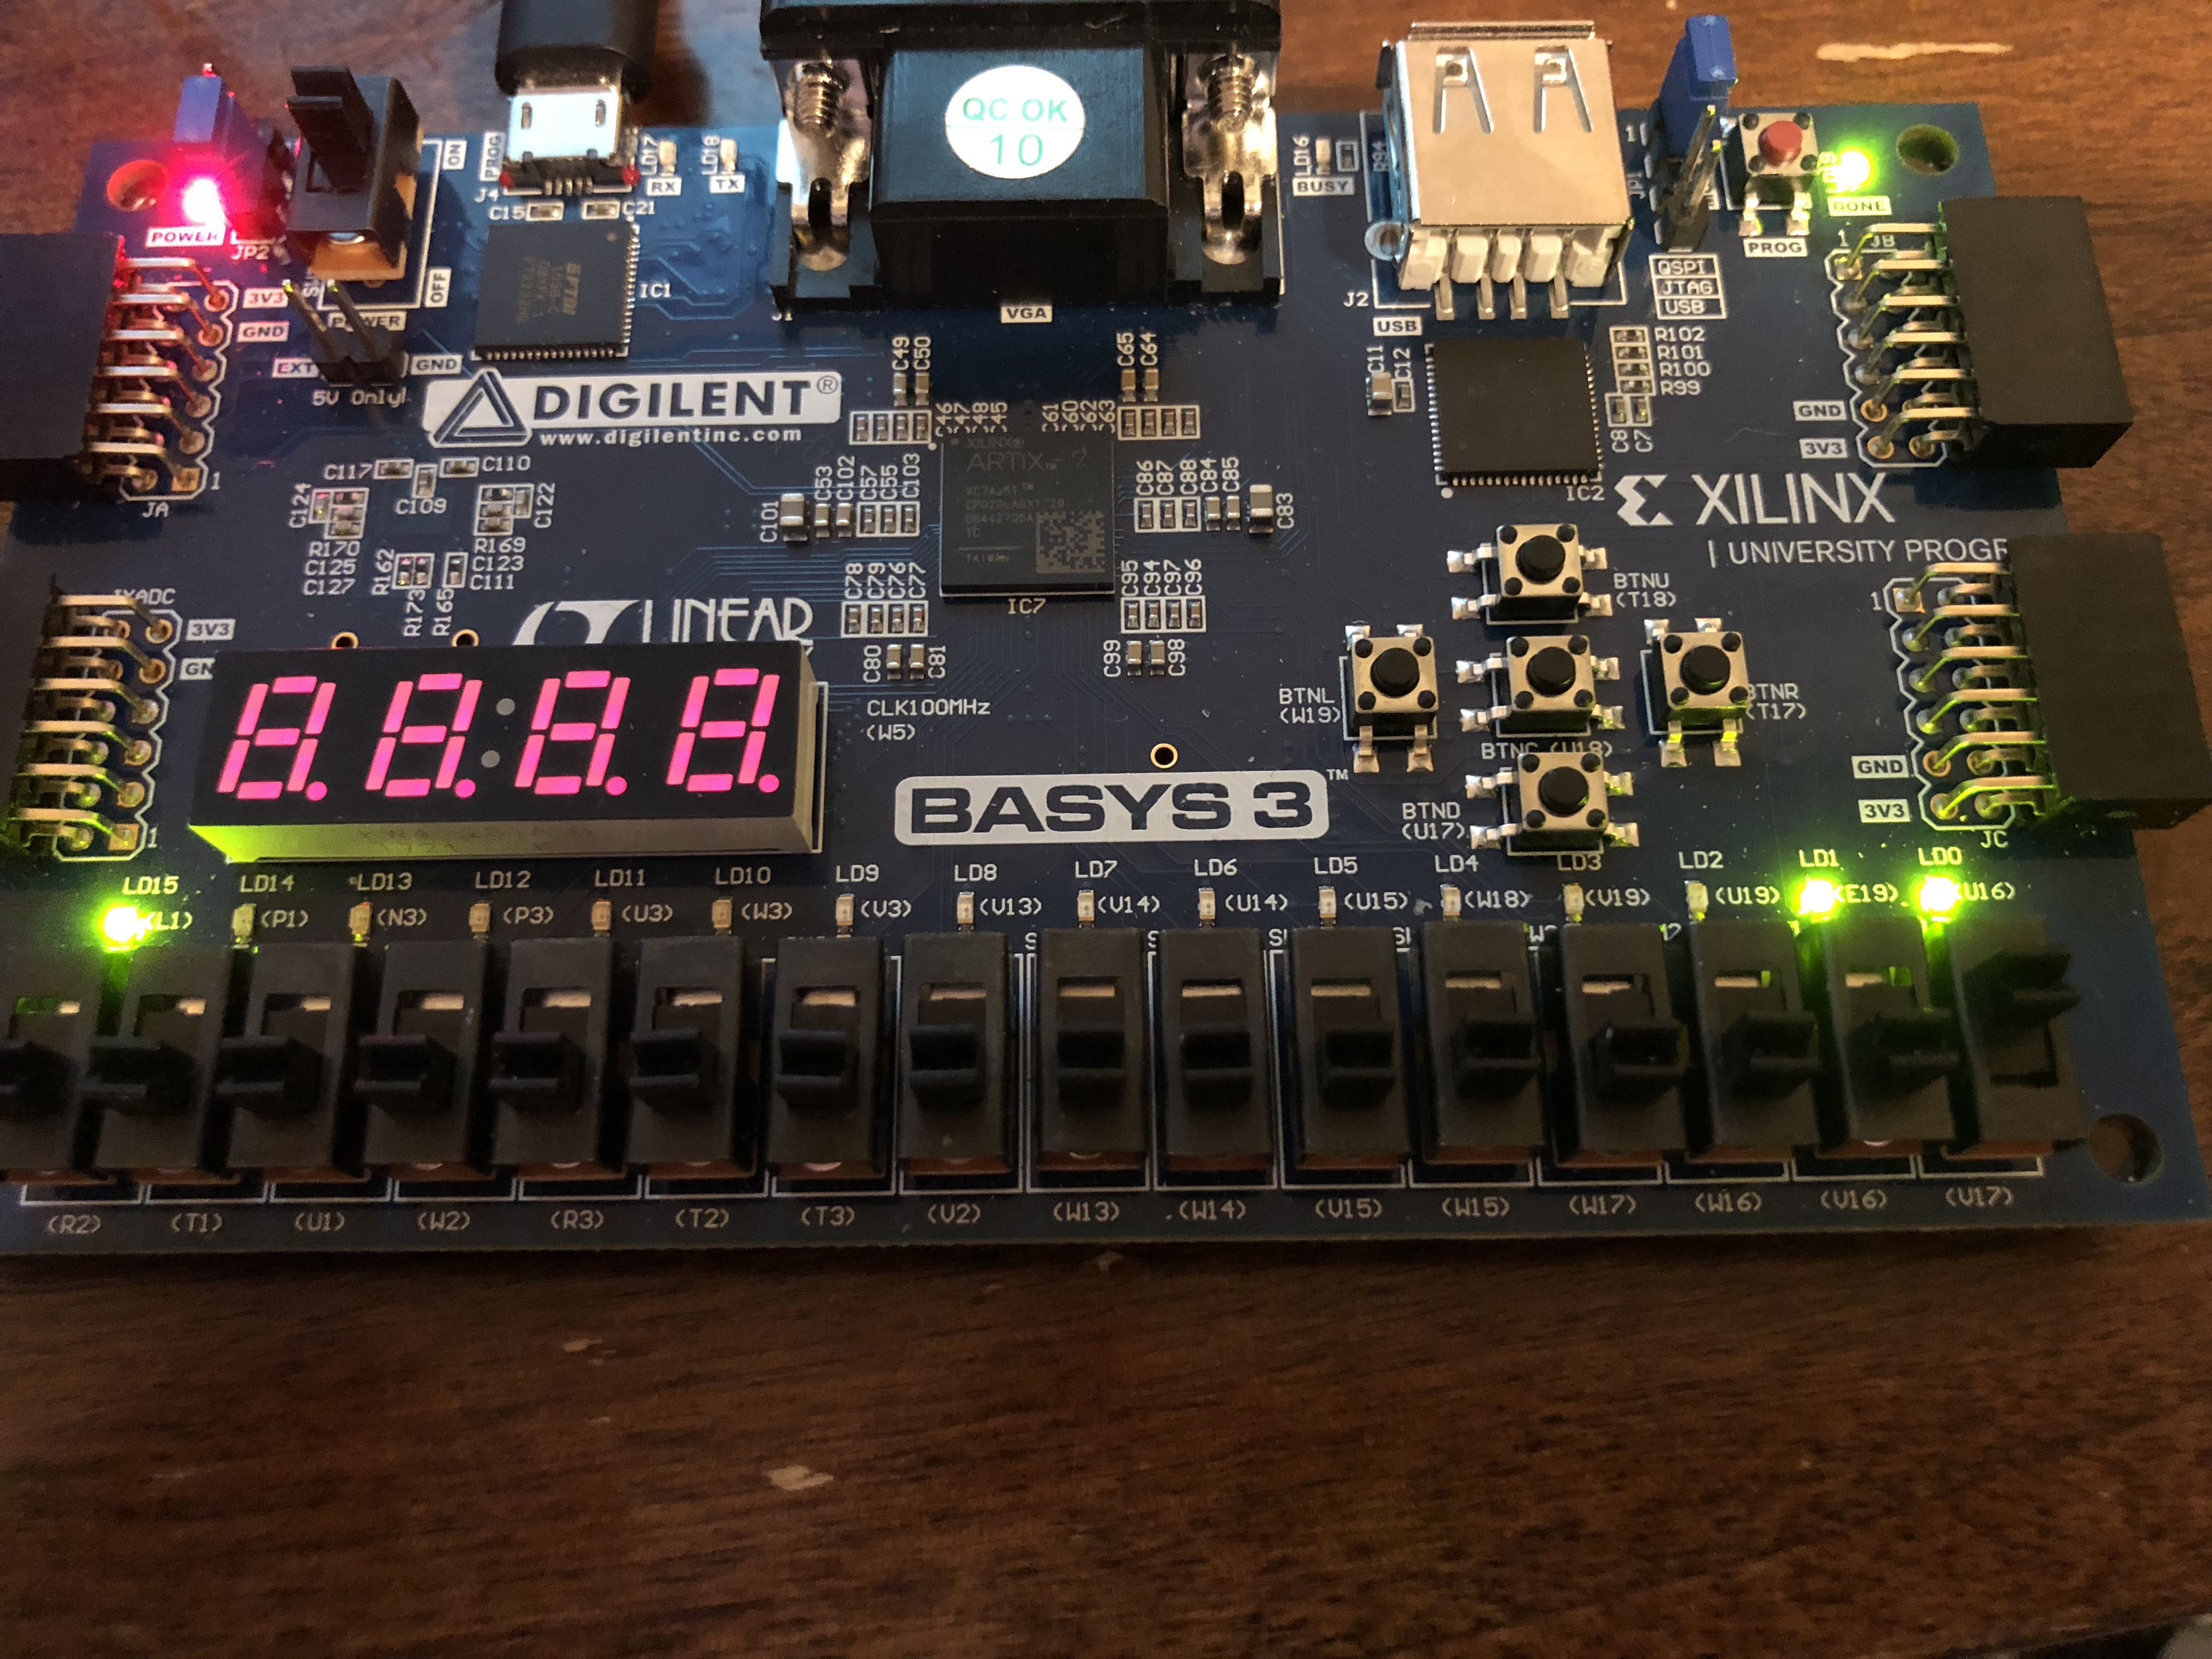
\includegraphics[width=0.5\textwidth]{./images/p2/IMG_1522.jpg}
	\caption{\label{fig:fsm_res4}FSM is in state 3.}
\end{center}
\end{figure}

\begin{figure}[H]
\begin{center}
	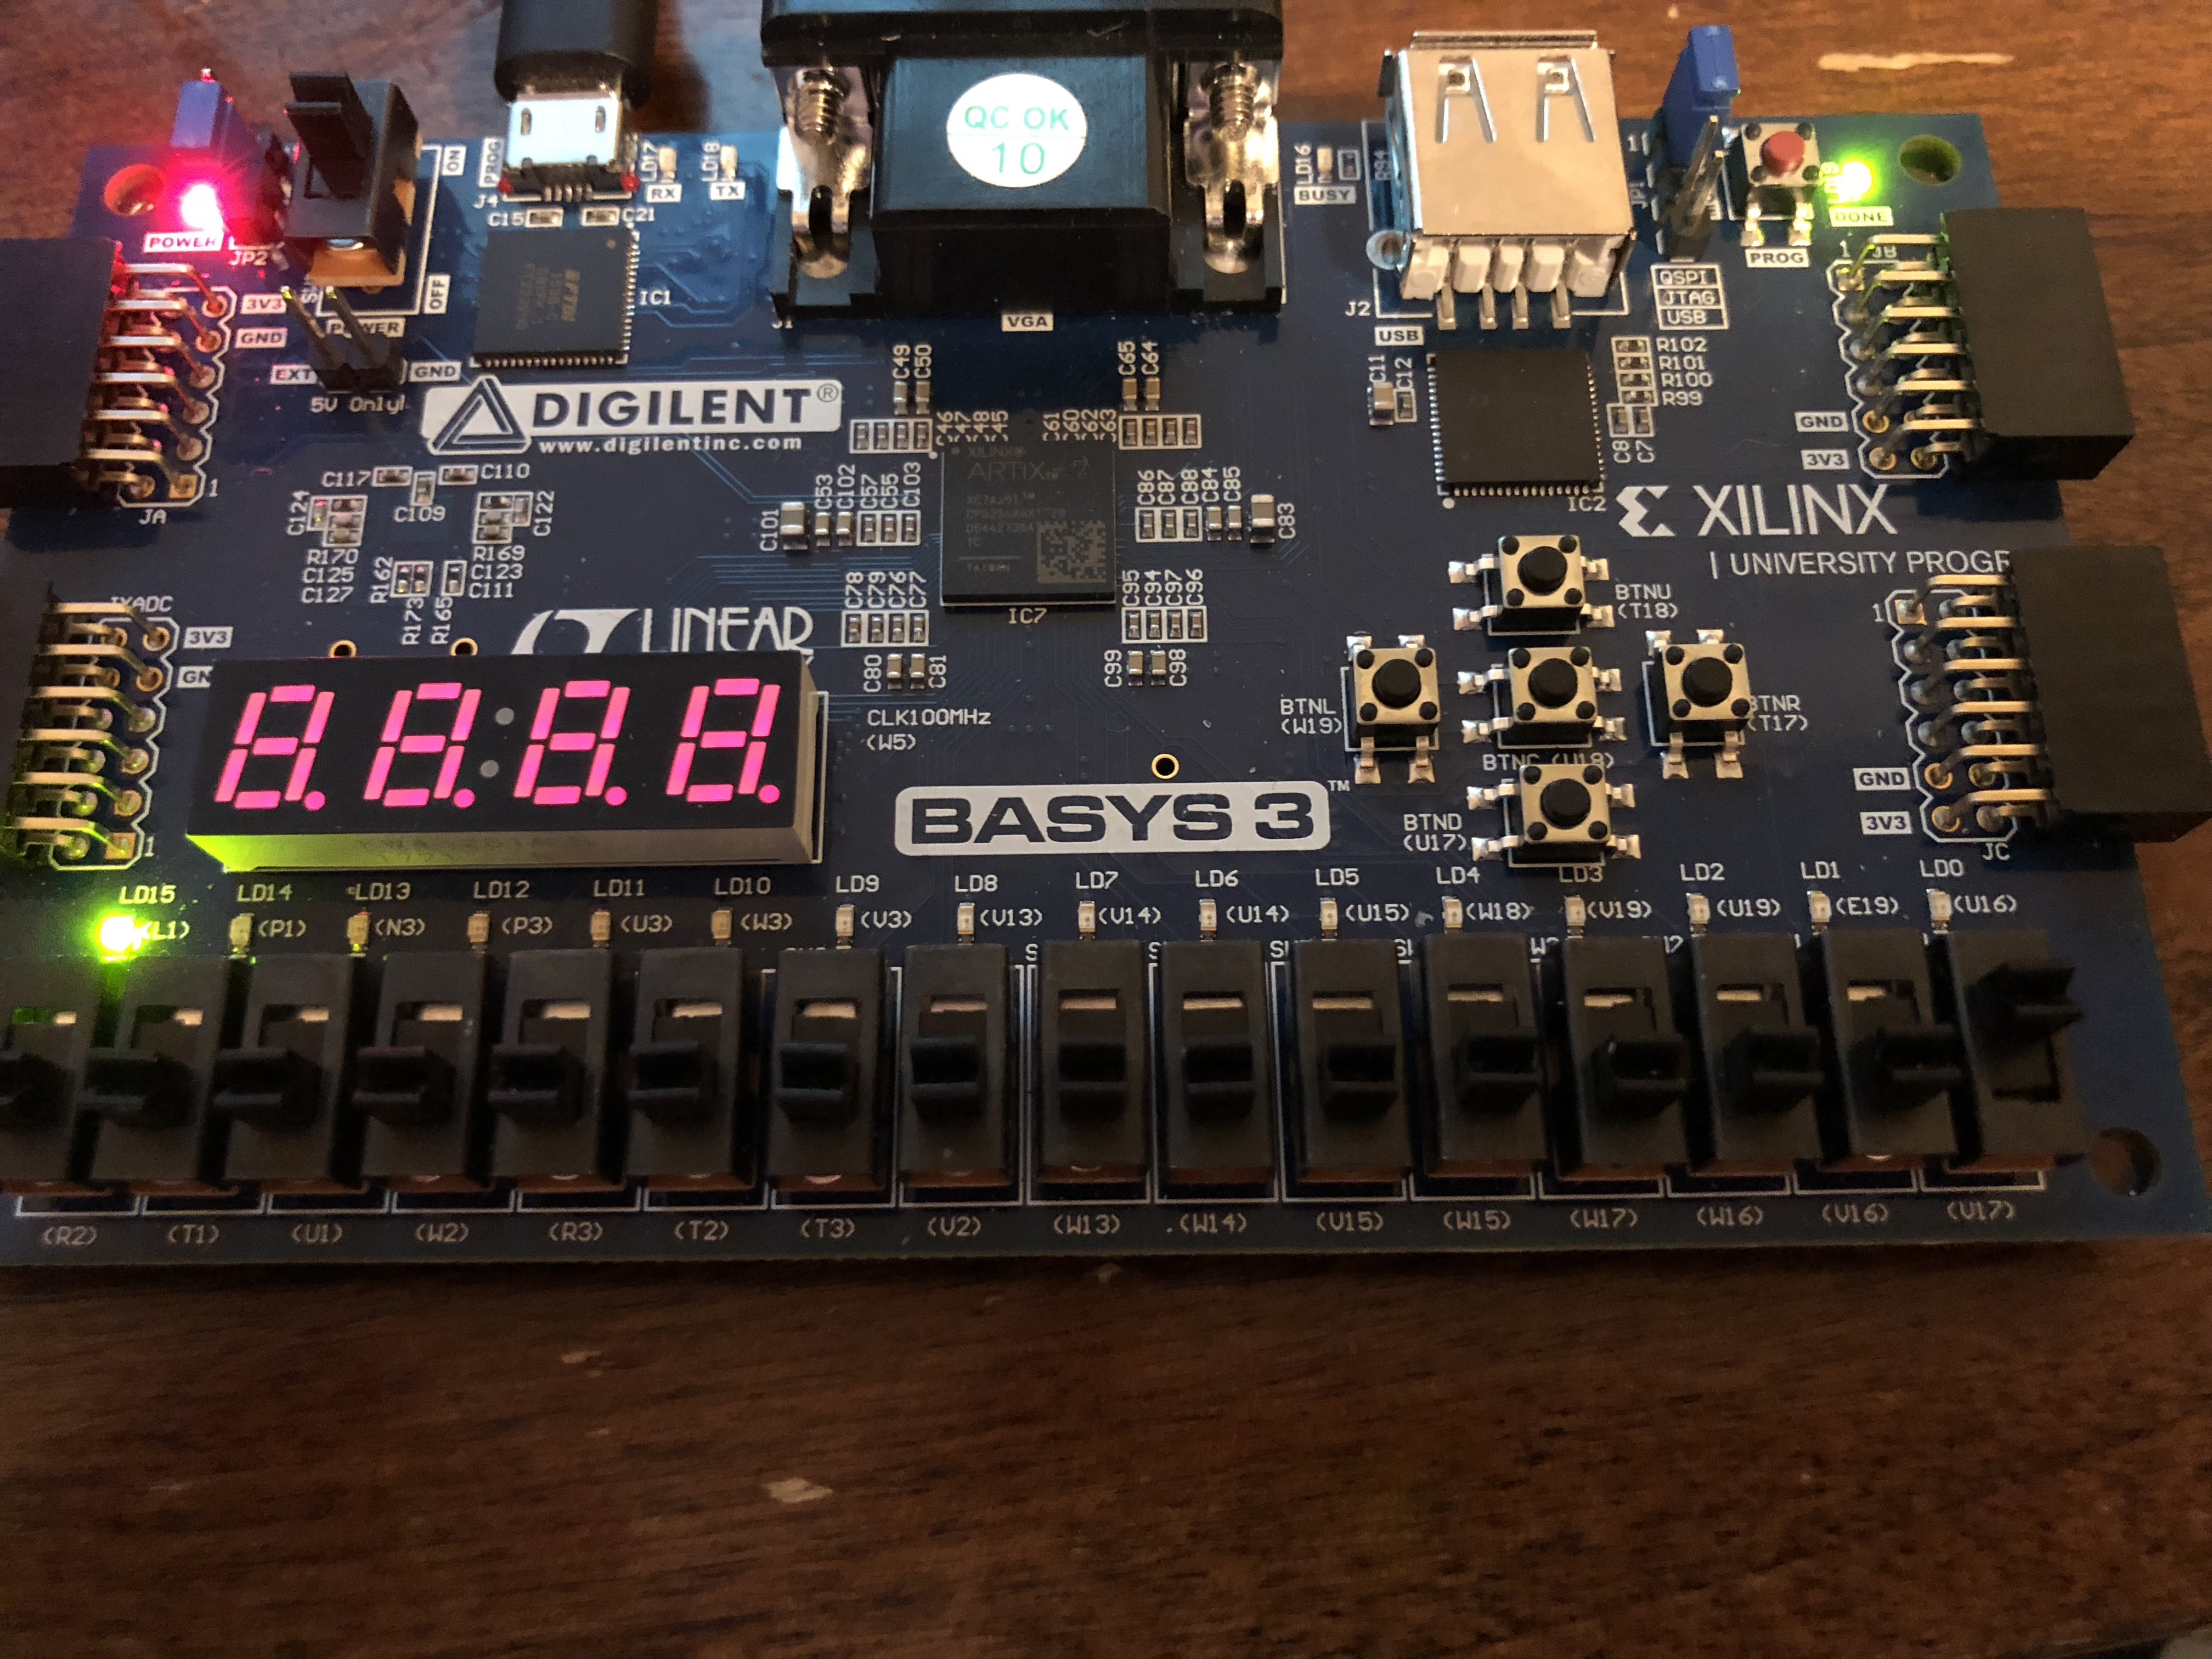
\includegraphics[width=0.5\textwidth]{./images/p2/IMG_1246.jpg}
	\caption{\label{fig:fsm_res5}FSM has returned to state 0.}
\end{center}
\end{figure}

\subsection{Problem 3}

\subsubsection{Background}
Problem 4 integrates the two units developed in the previous problem. We are to use the finite state machine to control the arithmetic state machine, cycling through each operation on the given inputs.

\subsubsection{Design Solution}
For our solution, we tied the output signal of the finite state machine to the select input for the arithmetic logic unit. This allows the unit to cycle through all possible operations for the given input. We also chose to show the current operation in our LEDs to help with debugging. The inputs and outputs for this design is shown in Tables ~\ref{tab:integrated_input_Ports} and ~\ref{tab:integration_output_Ports}, respectfully. The truth table for these operations is shown in Tables ~\ref{tab:integrated_truth_table1} and ~\ref{tab:integrated_truth_table2}.

\begin{table}[H]
\begin{center}
\begin{tabular}{| l | l | l |}
	\hline
	Bit & Label & Port \\ \hline
	in1[0] &  Switch 5 & V15 \\ \hline
	in1[1] & Switch 4 & w15 \\ \hline
	in2[0] & Switch 3 & W16 \\ \hline
	in2[1] & Switch 2 & W17 \\ \hline
	clk &  Clock & W5 \\ \hline
	enable & Switch 0 & V17 \\ \hline
	reset & Button Right & T17 \\ \hline
\end{tabular}
\caption{\label{tab:integration_input_Ports}Input port assignments for  the integrated circuit.}
\end{center}
\end{table}

\begin{table}[H]
\begin{center}
\begin{tabular}{| l | l | l |}
	\hline
	Bit & Label & Port \\ \hline
	output[0] & LED 0 & U16 \\ \hline
	output[1] & LED 1 & E19 \\ \hline
	operation[0] & & U19 \\ \hline
	operation[1] & & V19 \\ \hline
\end{tabular}
\caption{\label{tab:integration_output_Ports}Output port assignments for the integrated circuit.}
\end{center}
\end{table}

\begin{table}[H]
\begin{center}
\begin{tabular}{| l | l | l | l |}
	\hline
	in1 & in2 & state(sel) & output \\ \hline
	00 & 00 & 00 & 00 \\ \hline
	00 & 00 & 01 & 00 \\ \hline
	00 & 00 & 10 & 00 \\ \hline
	00 & 00 & 11 & 00 \\ \hline
	00 & 01 & 00 & 00 \\ \hline
	00 & 01 & 01 & 01 \\ \hline
	00 & 01 & 10 & 00 \\ \hline
	00 & 01 & 11 & 00 \\ \hline
	00 & 10 & 00 & 00 \\ \hline
	00 & 10 & 01 & 10 \\ \hline
	00 & 10 & 10 & 00 \\ \hline
	00 & 10 & 11 & 00 \\ \hline
	00 & 11 & 00 & 00 \\ \hline
	00 & 11 & 01 & 11 \\ \hline
	00 & 11 & 10 & 00 \\ \hline
	00 & 11 & 11 & 00 \\ \hline
	01 & 00 & 00 & 00 \\ \hline
	01 & 00 & 01 & 01 \\ \hline
	01 & 00 & 10 & 01 \\ \hline
	01 & 00 & 11 & 01 \\ \hline
	01 & 01 & 00 & 01 \\ \hline
	01 & 01 & 01 & 01 \\ \hline
	01 & 01 & 10 & 00 \\ \hline
	01 & 01 & 11 & 10 \\ \hline
	01 & 10 & 00 & 00 \\ \hline
	01 & 10 & 01 & 11 \\ \hline
	01 & 10 & 10 & 00 \\ \hline
	01 & 10 & 11 & 00 \\ \hline
	01 & 11 & 00 & 01 \\ \hline
	01 & 11 & 01 & 11 \\ \hline
	01 & 11 & 10 & 00 \\ \hline
	01 & 11 & 11 & 00 \\ \hline
\end{tabular}
\caption{\label{tab:integrated_truth_table1}Truth table for each set of given inputs in each possible state part 1.}
\end{center}
\end{table}

\begin{table}[H]
\begin{center}
\begin{tabular}{| l | l | l | l |}
	\hline
	in1 & in2 & state(sel) & output \\ \hline
	10 & 00 & 00 & 00 \\ \hline
	10 & 00 & 01 & 10 \\ \hline
	10 & 00 & 10 & 10 \\ \hline
	10 & 00 & 11 & 10 \\ \hline
	10 & 01 & 00 & 00 \\ \hline
	10 & 01 & 01 & 11 \\ \hline
	10 & 01 & 10 & 01 \\ \hline
	10 & 01 & 11 & 00 \\ \hline
	10 & 10 & 00 & 10 \\ \hline
	10 & 10 & 01 & 10 \\ \hline
	10 & 10 & 10 & 00 \\ \hline
	10 & 10 & 11 & 00 \\ \hline
	10 & 11 & 00 & 10 \\ \hline
	10 & 11 & 01 & 11 \\ \hline
	10 & 11 & 10 & 00 \\ \hline
	10 & 11 & 11 & 00 \\ \hline
	11 & 00 & 00 & 00 \\ \hline
	11 & 00 & 01 & 11 \\ \hline
	11 & 00 & 10 & 11 \\ \hline
	11 & 00 & 11 & 11 \\ \hline
	11 & 01 & 00 & 01 \\ \hline
	11 & 01 & 01 & 11 \\ \hline
	11 & 01 & 10 & 01 \\ \hline
	11 & 01 & 11 & 10 \\ \hline
	11 & 10 & 00 & 10 \\ \hline
	11 & 10 & 01 & 11 \\ \hline
	11 & 10 & 10 & 00 \\ \hline
	11 & 10 & 11 & 00 \\ \hline
	11 & 11 & 00 & 11 \\ \hline
	11 & 11 & 01 & 11 \\ \hline
	11 & 11 & 10 & 00 \\ \hline
	11 & 11 & 11 & 00 \\ \hline
\end{tabular}
\caption{\label{tab:integrated_truth_table2}Truth table for each set of given inputs in each possible state part 2.}
\end{center}
\end{table}

\subsubsection{Results}
\begin{figure}[H]
\begin{center}
	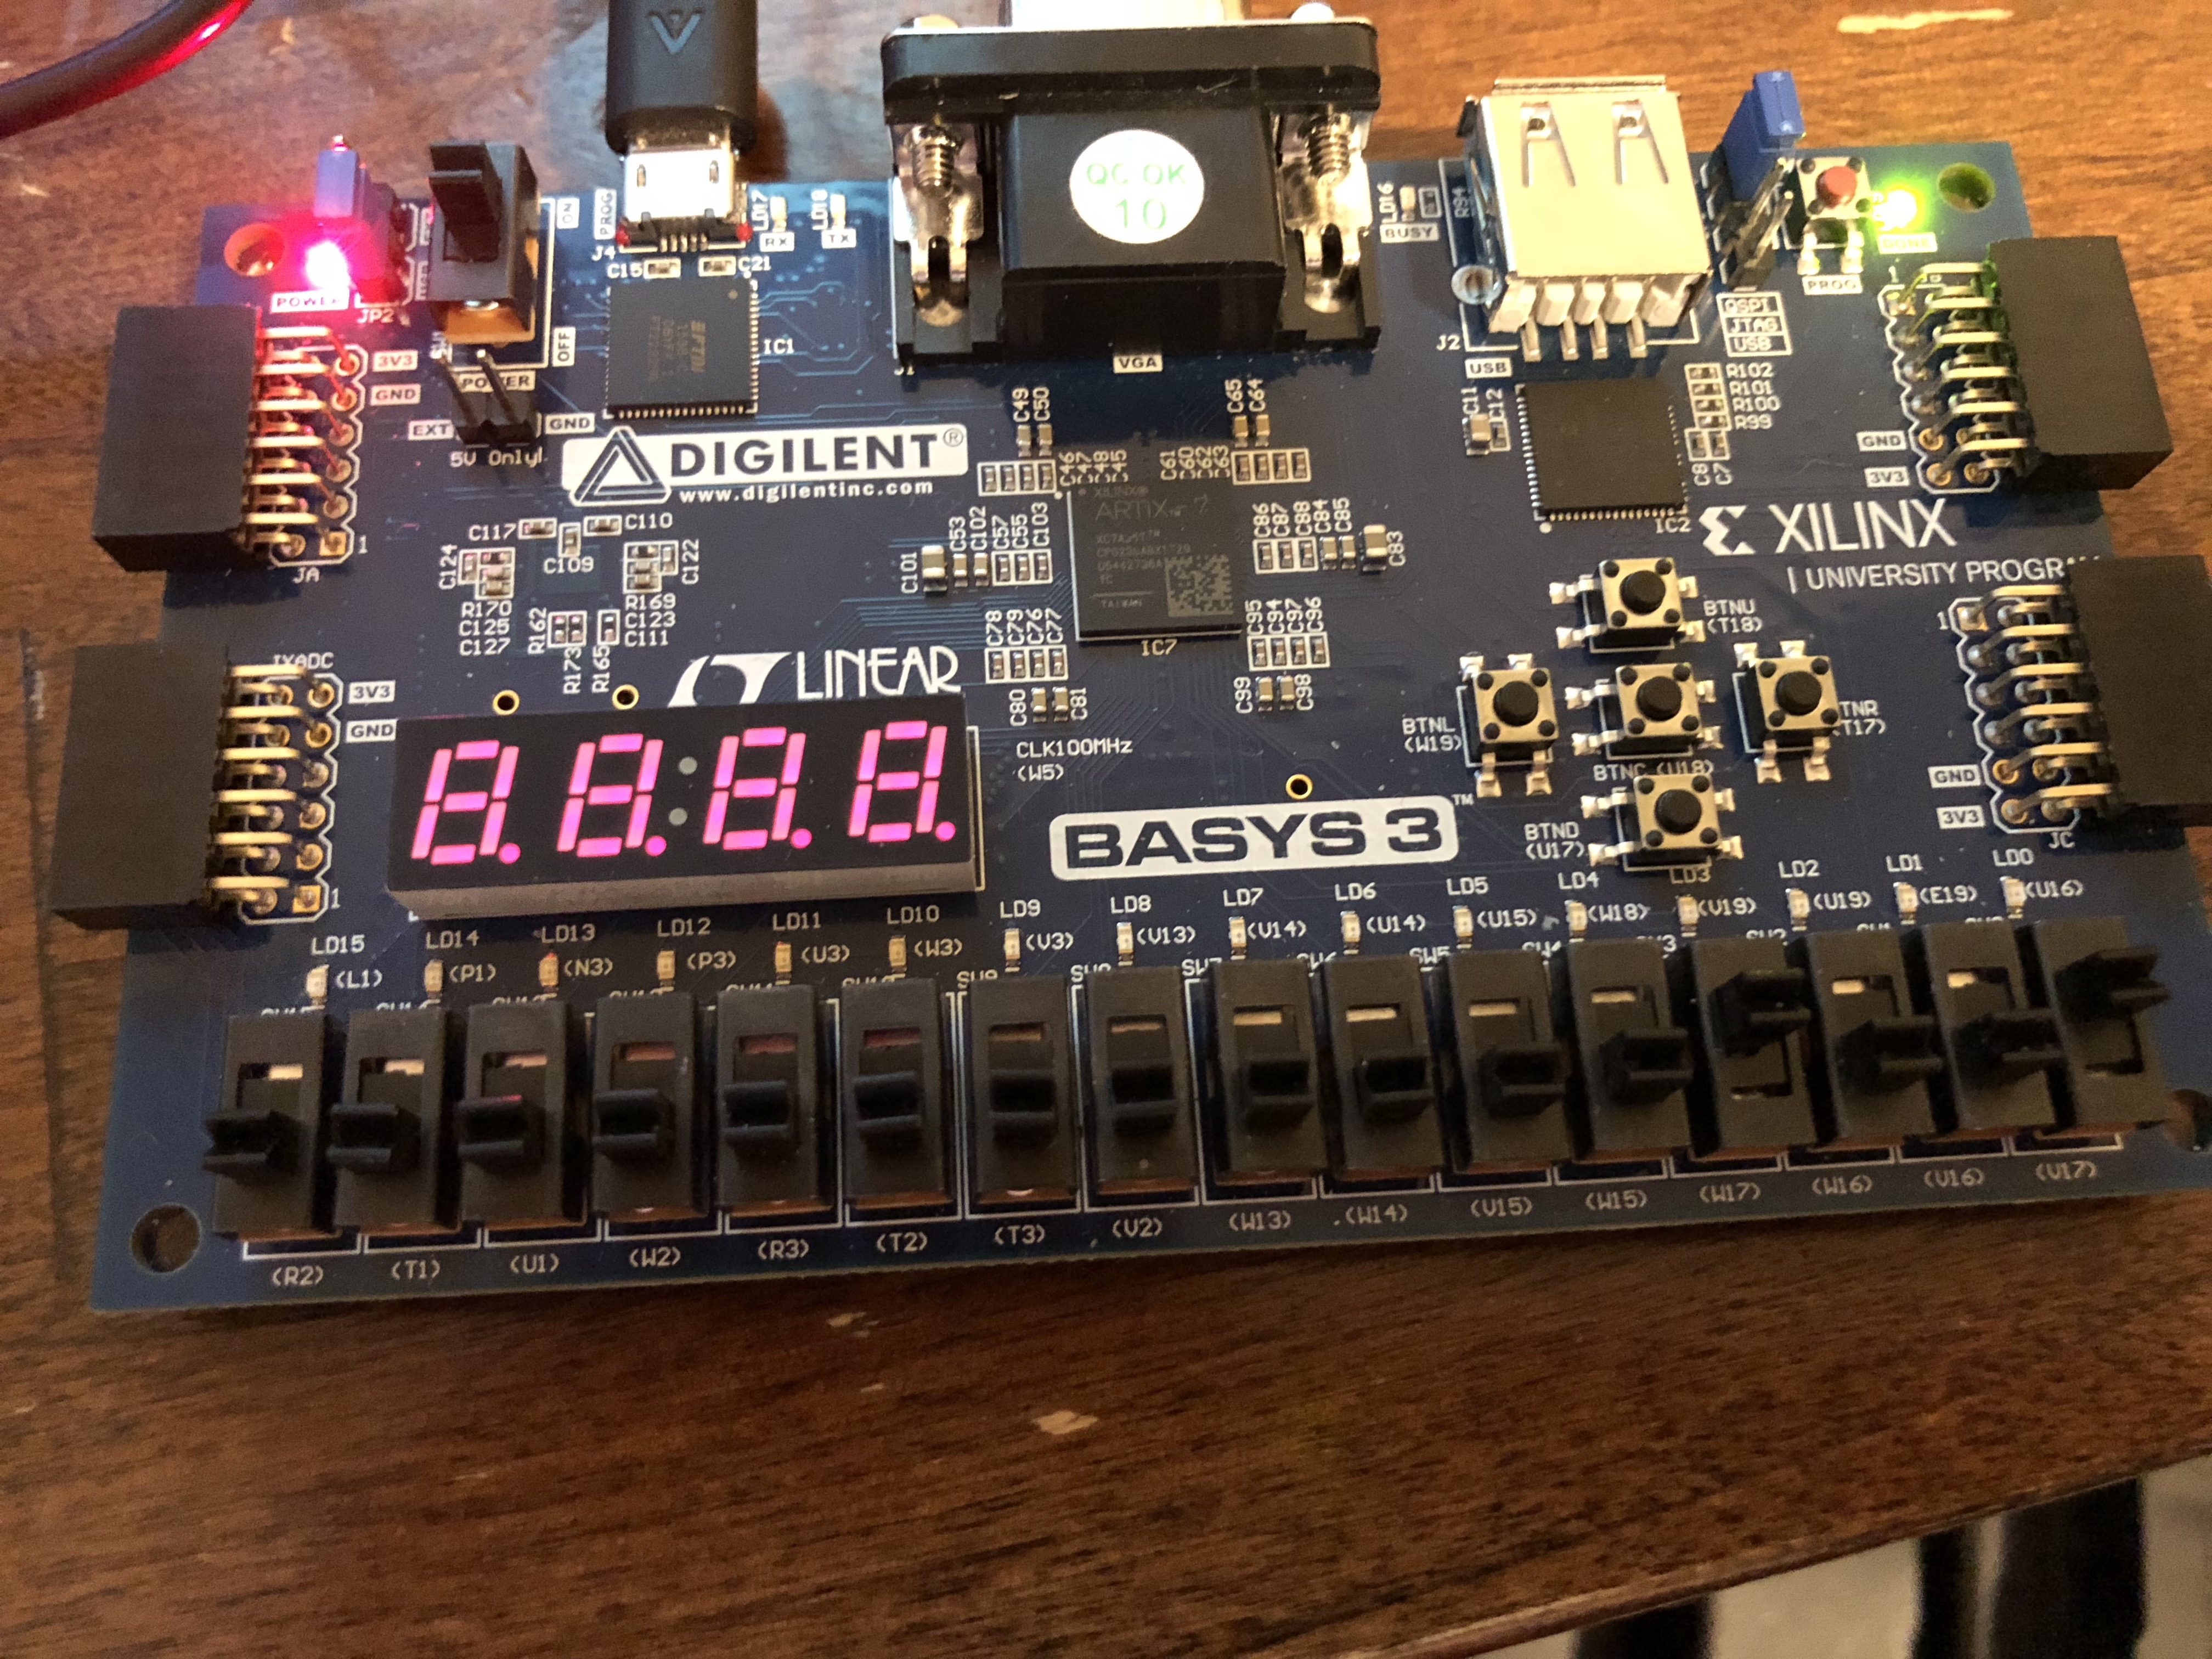
\includegraphics[width=0.5\textwidth]{./images/p3/IMG_1555.jpg}
	\caption{\label{fig:int_res1}FSM is in state 0 with input 0, 10 AND 01 = 00.}
\end{center}
\end{figure}

\begin{figure}[H]
\begin{center}
	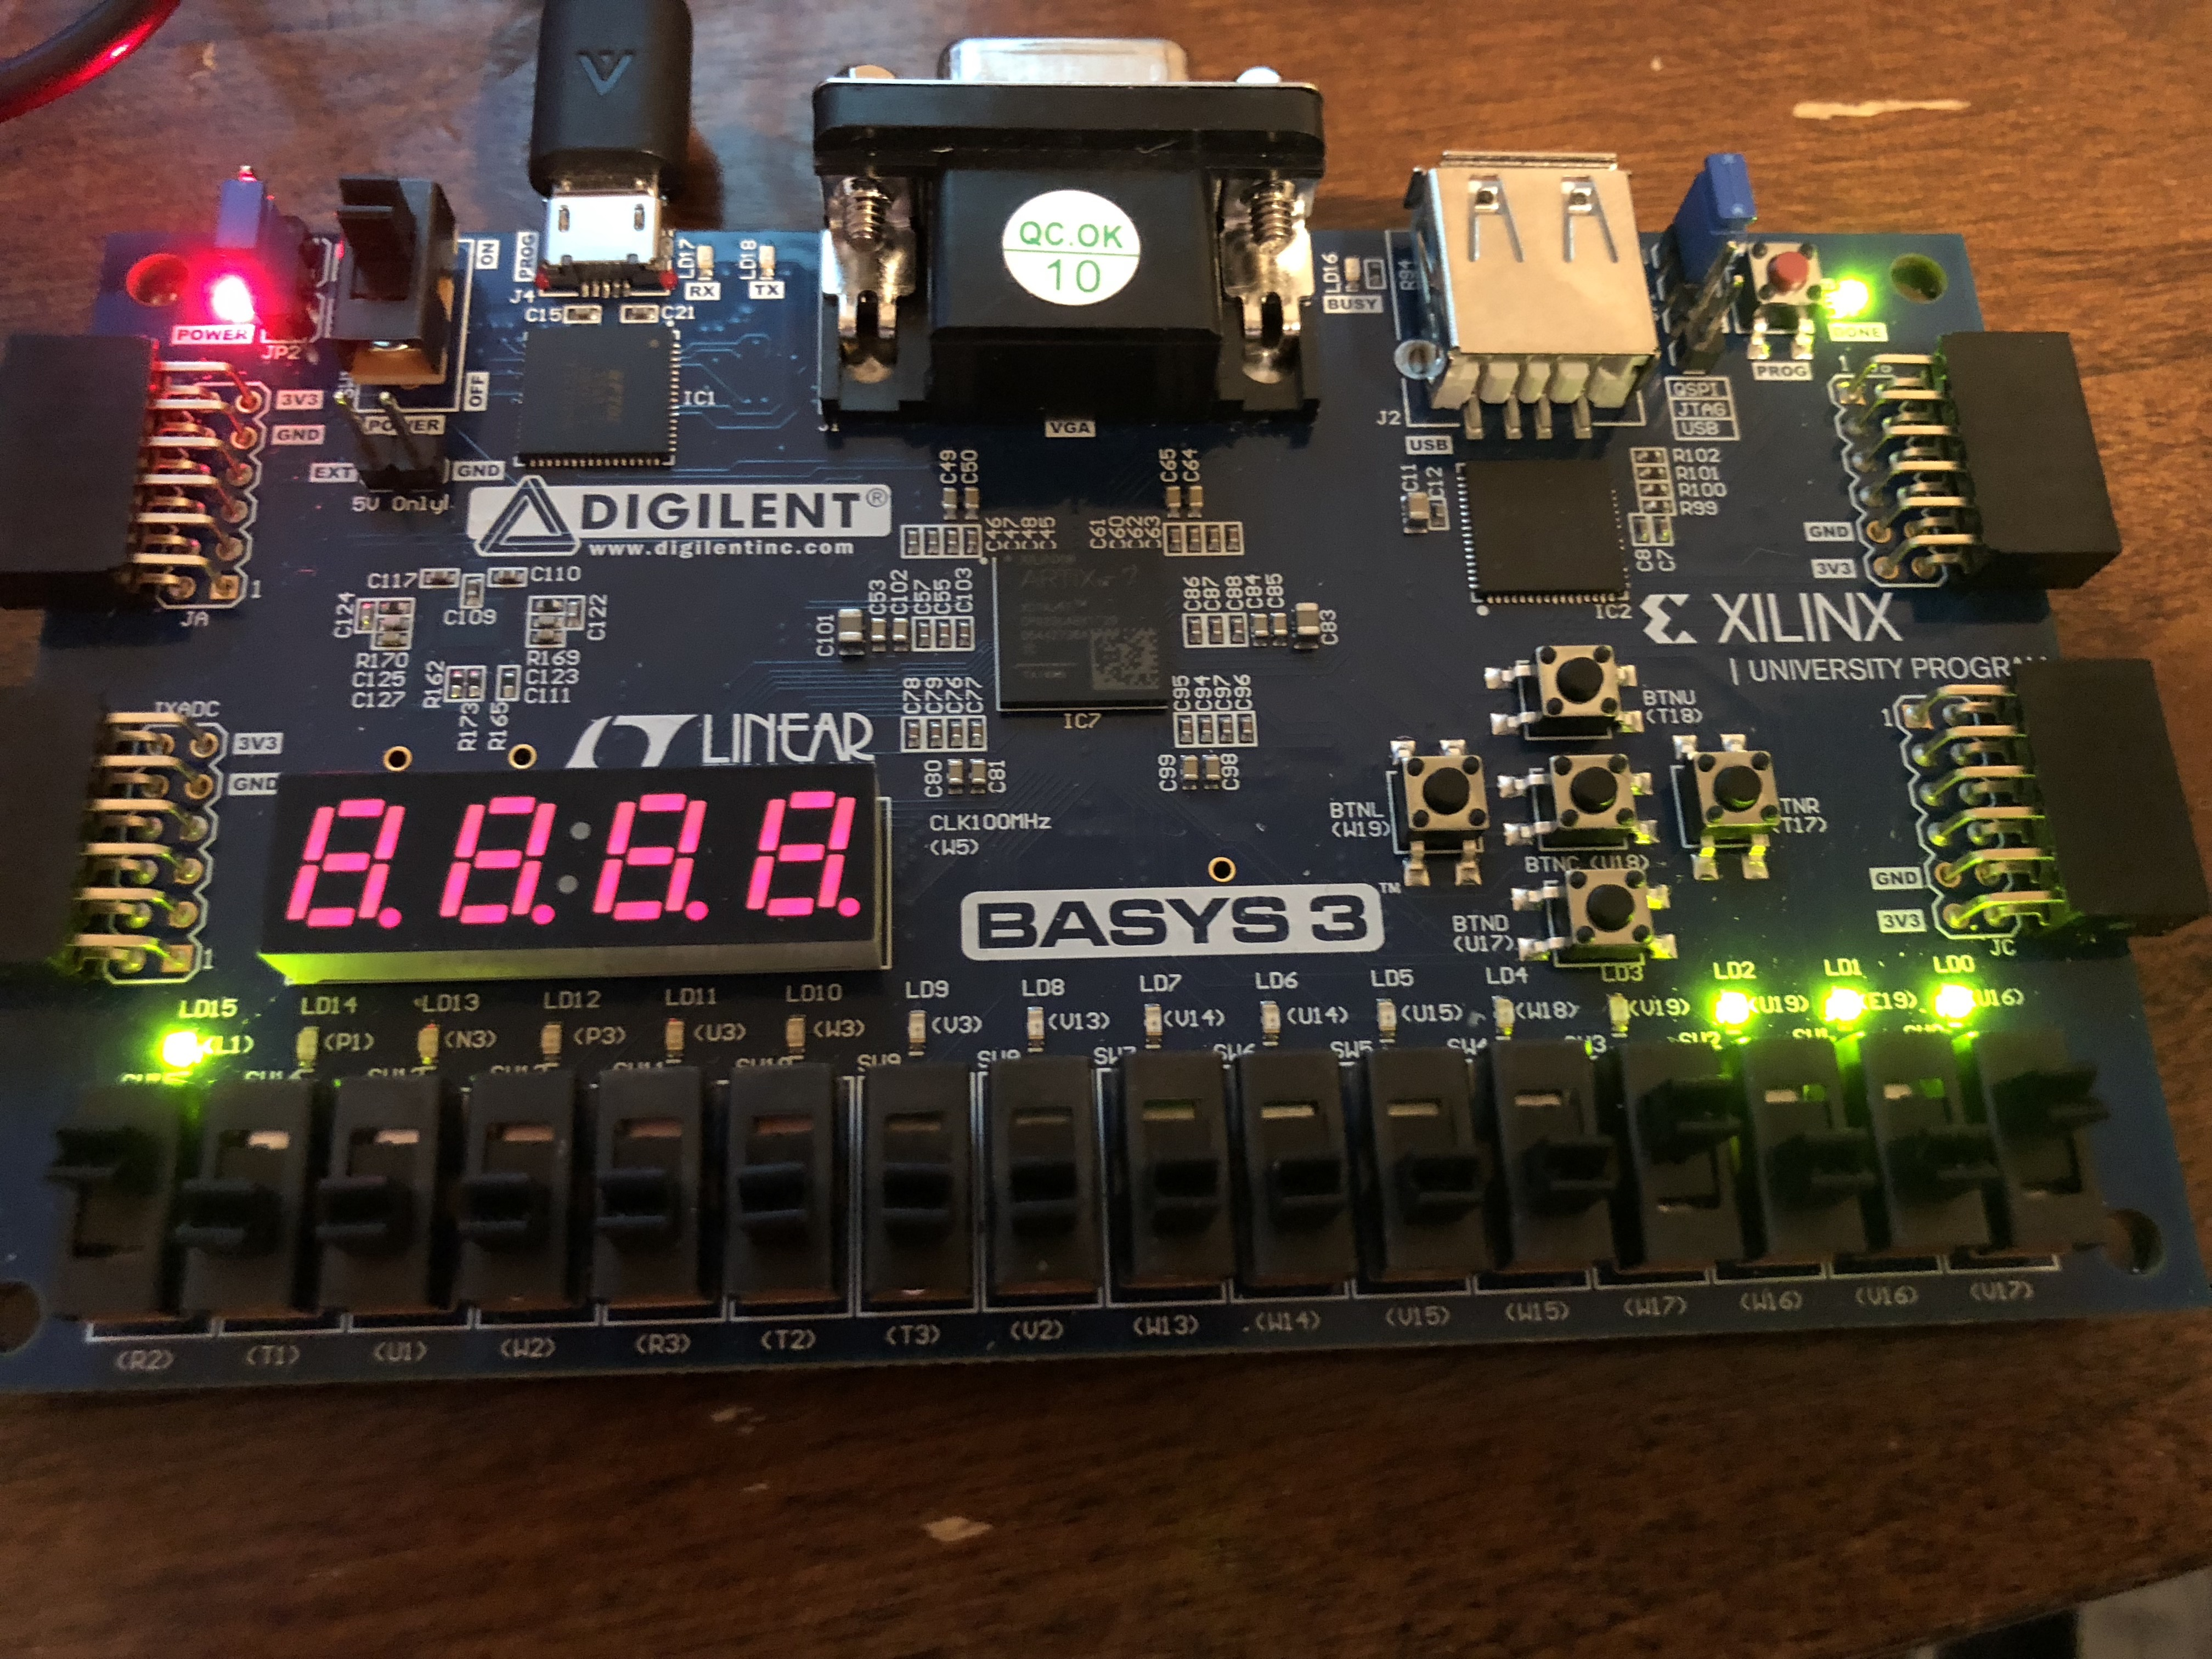
\includegraphics[width=0.5\textwidth]{./images/p3/IMG_9868.jpg}
	\caption{\label{fig:int_res2}FSM is in state 1 with output 11, 10 OR 01 = 11.}
\end{center}
\end{figure}

\begin{figure}[H]
\begin{center}
	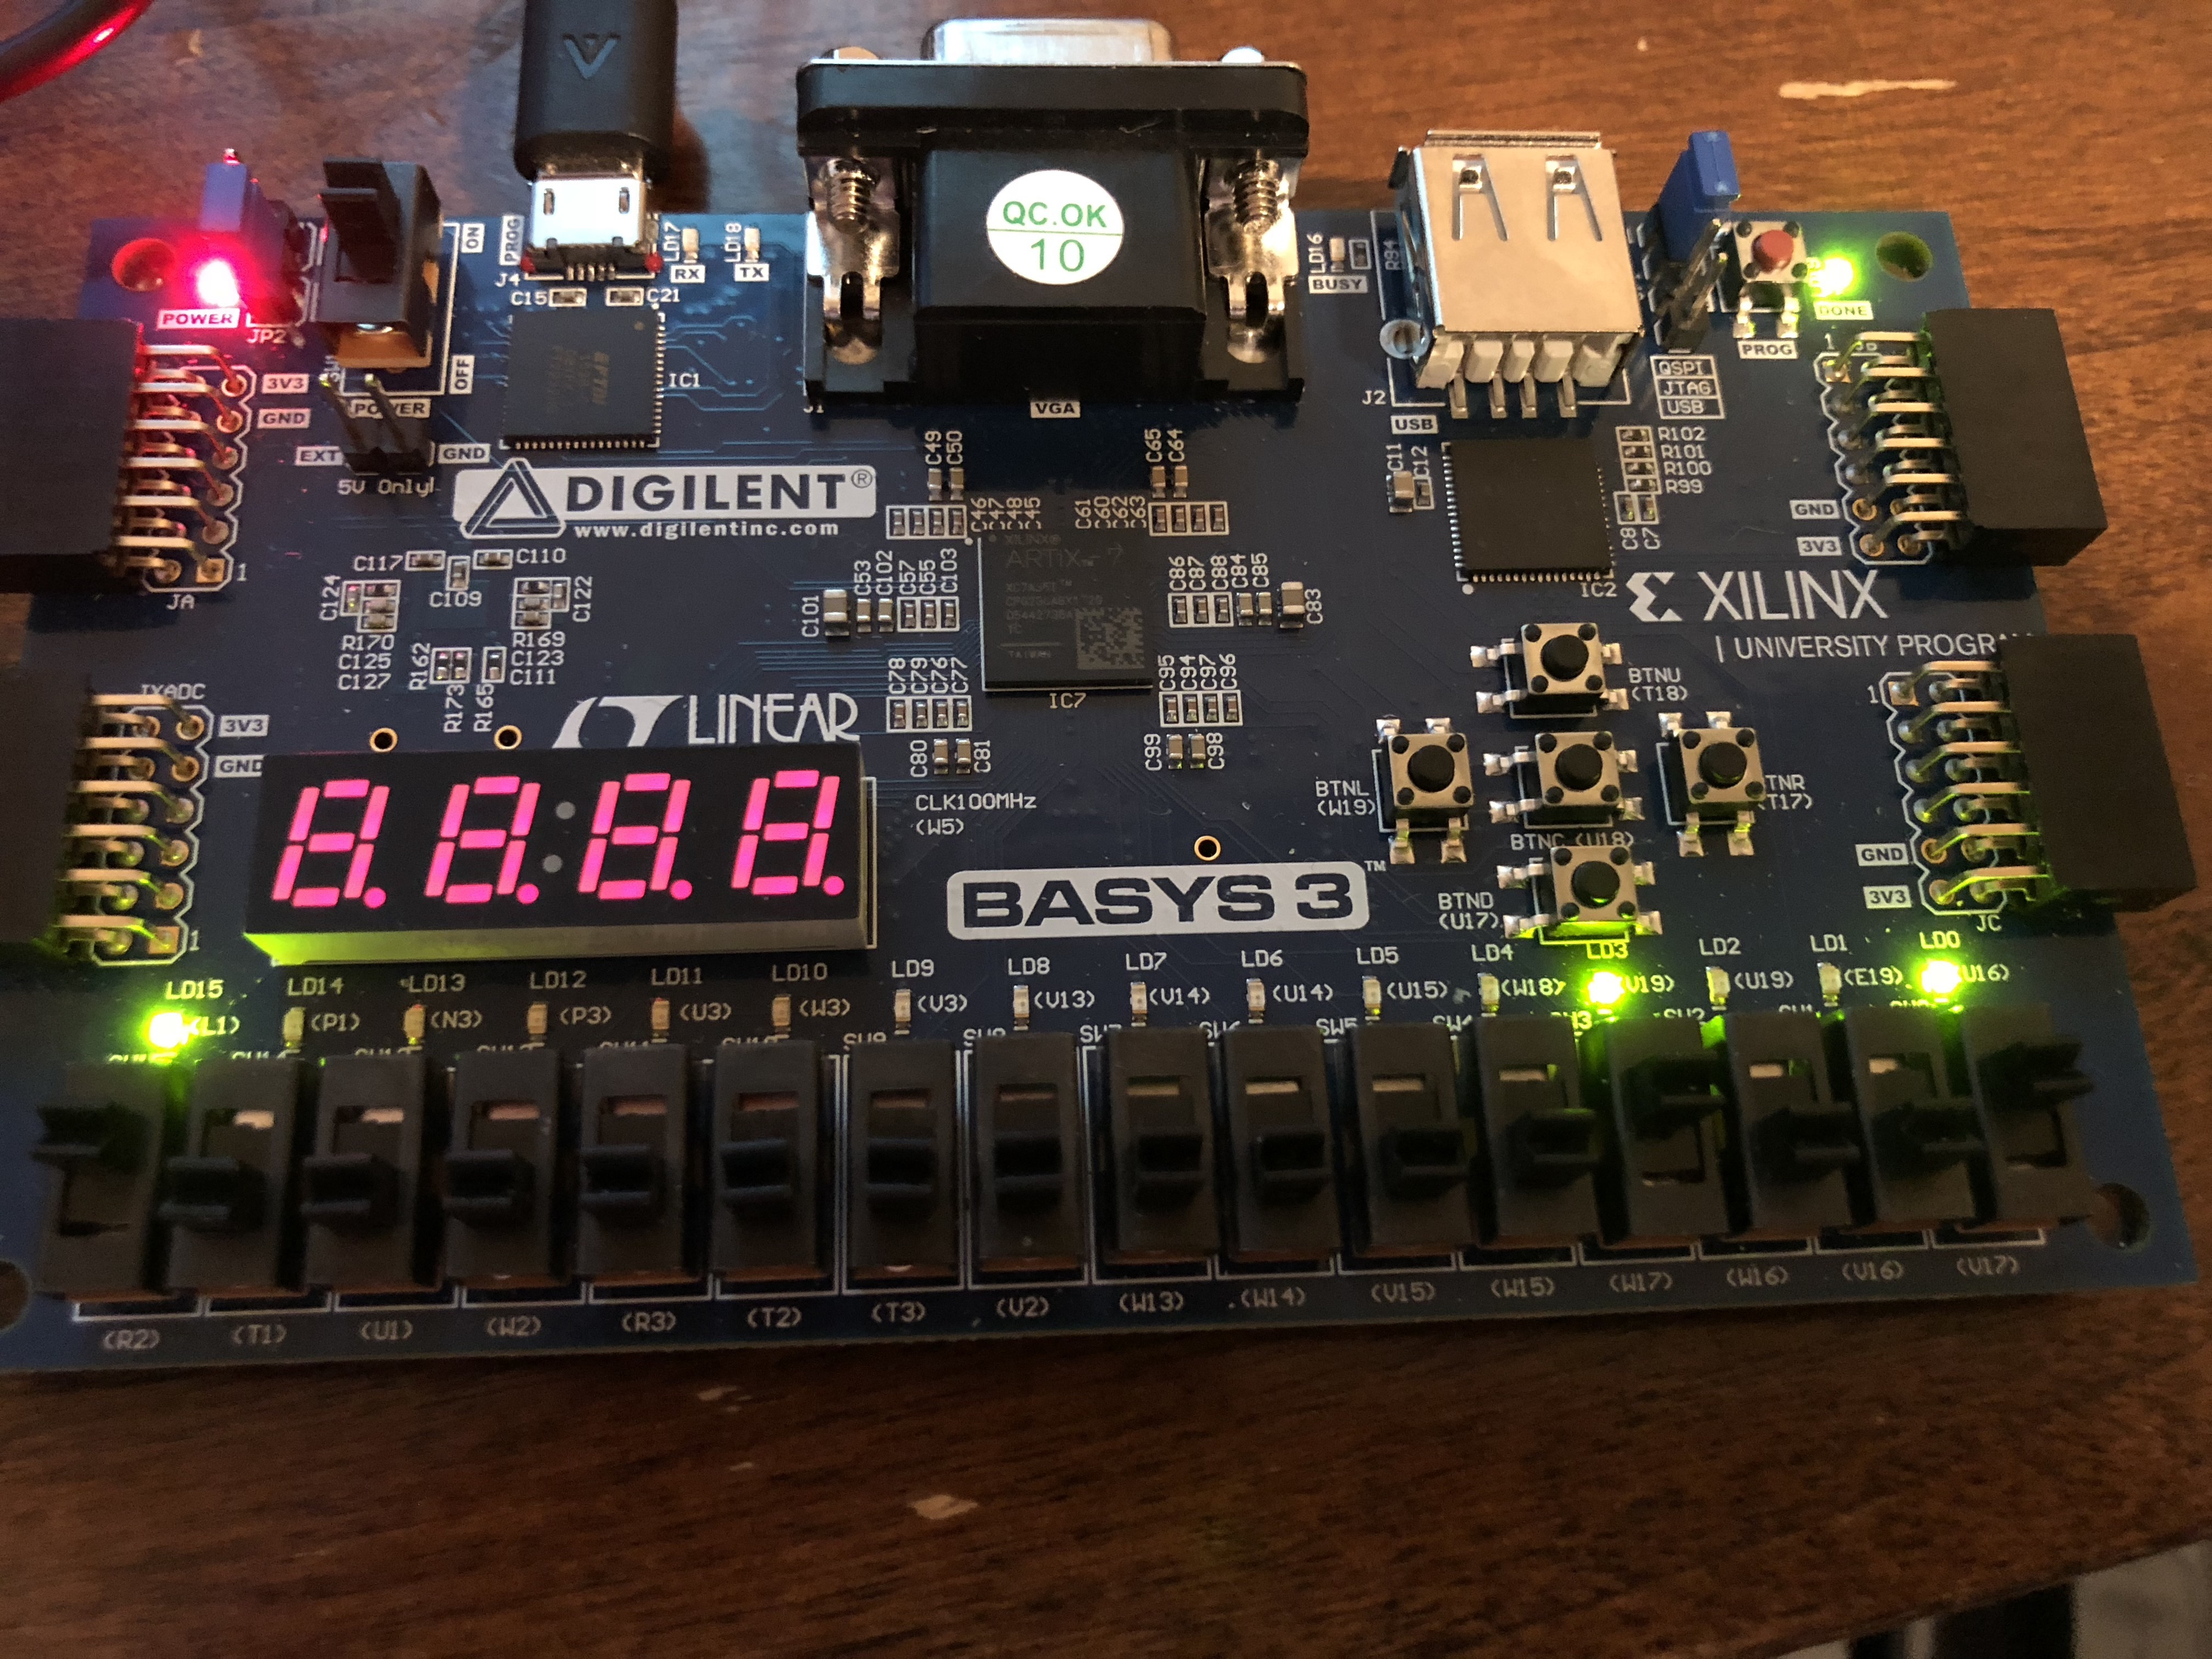
\includegraphics[width=0.5\textwidth]{./images/p3/IMG_4430.jpg}
	\caption{\label{fig:int_res3}FSM is in state 2. 10 shift right by 01 =01.}
\end{center}
\end{figure}

\begin{figure}[H]
\begin{center}
	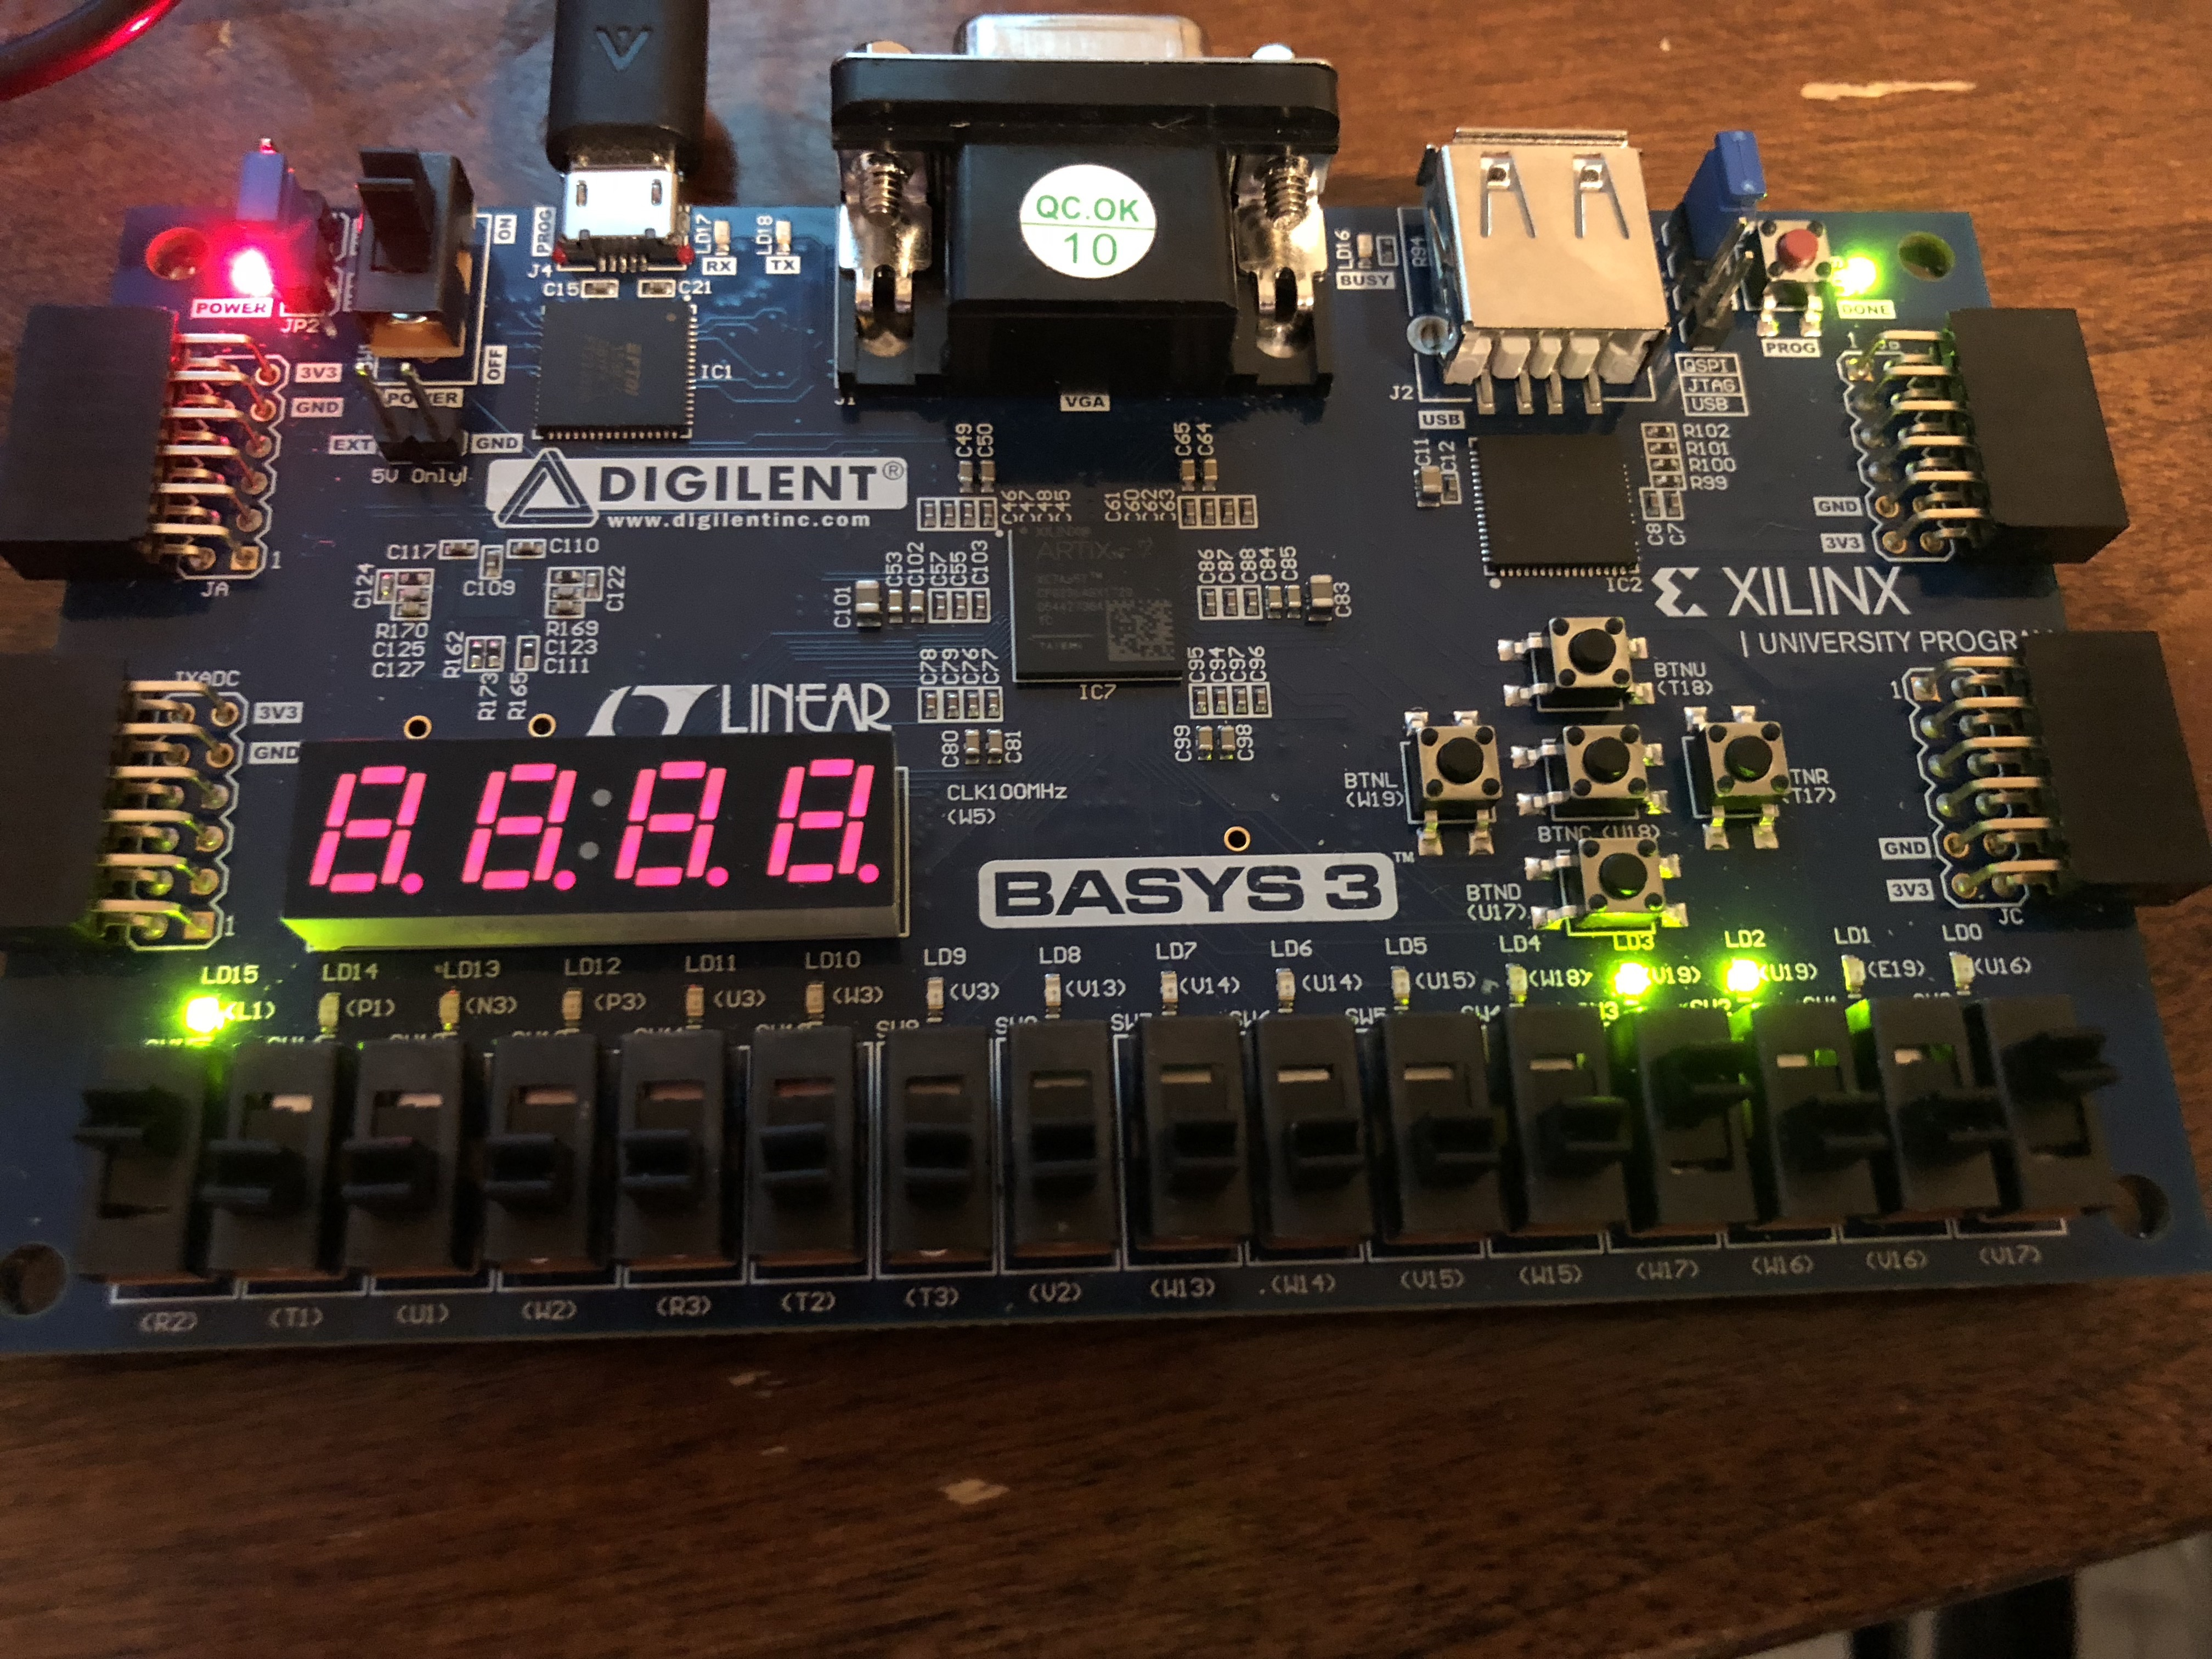
\includegraphics[width=0.5\textwidth]{./images/p3/IMG_0945.jpg}
	\caption{\label{fig:int_res4}FSM is in state 3. 10 shift left by 01 = 00.}
\end{center}
\end{figure}

\begin{figure}[H]
\begin{center}
	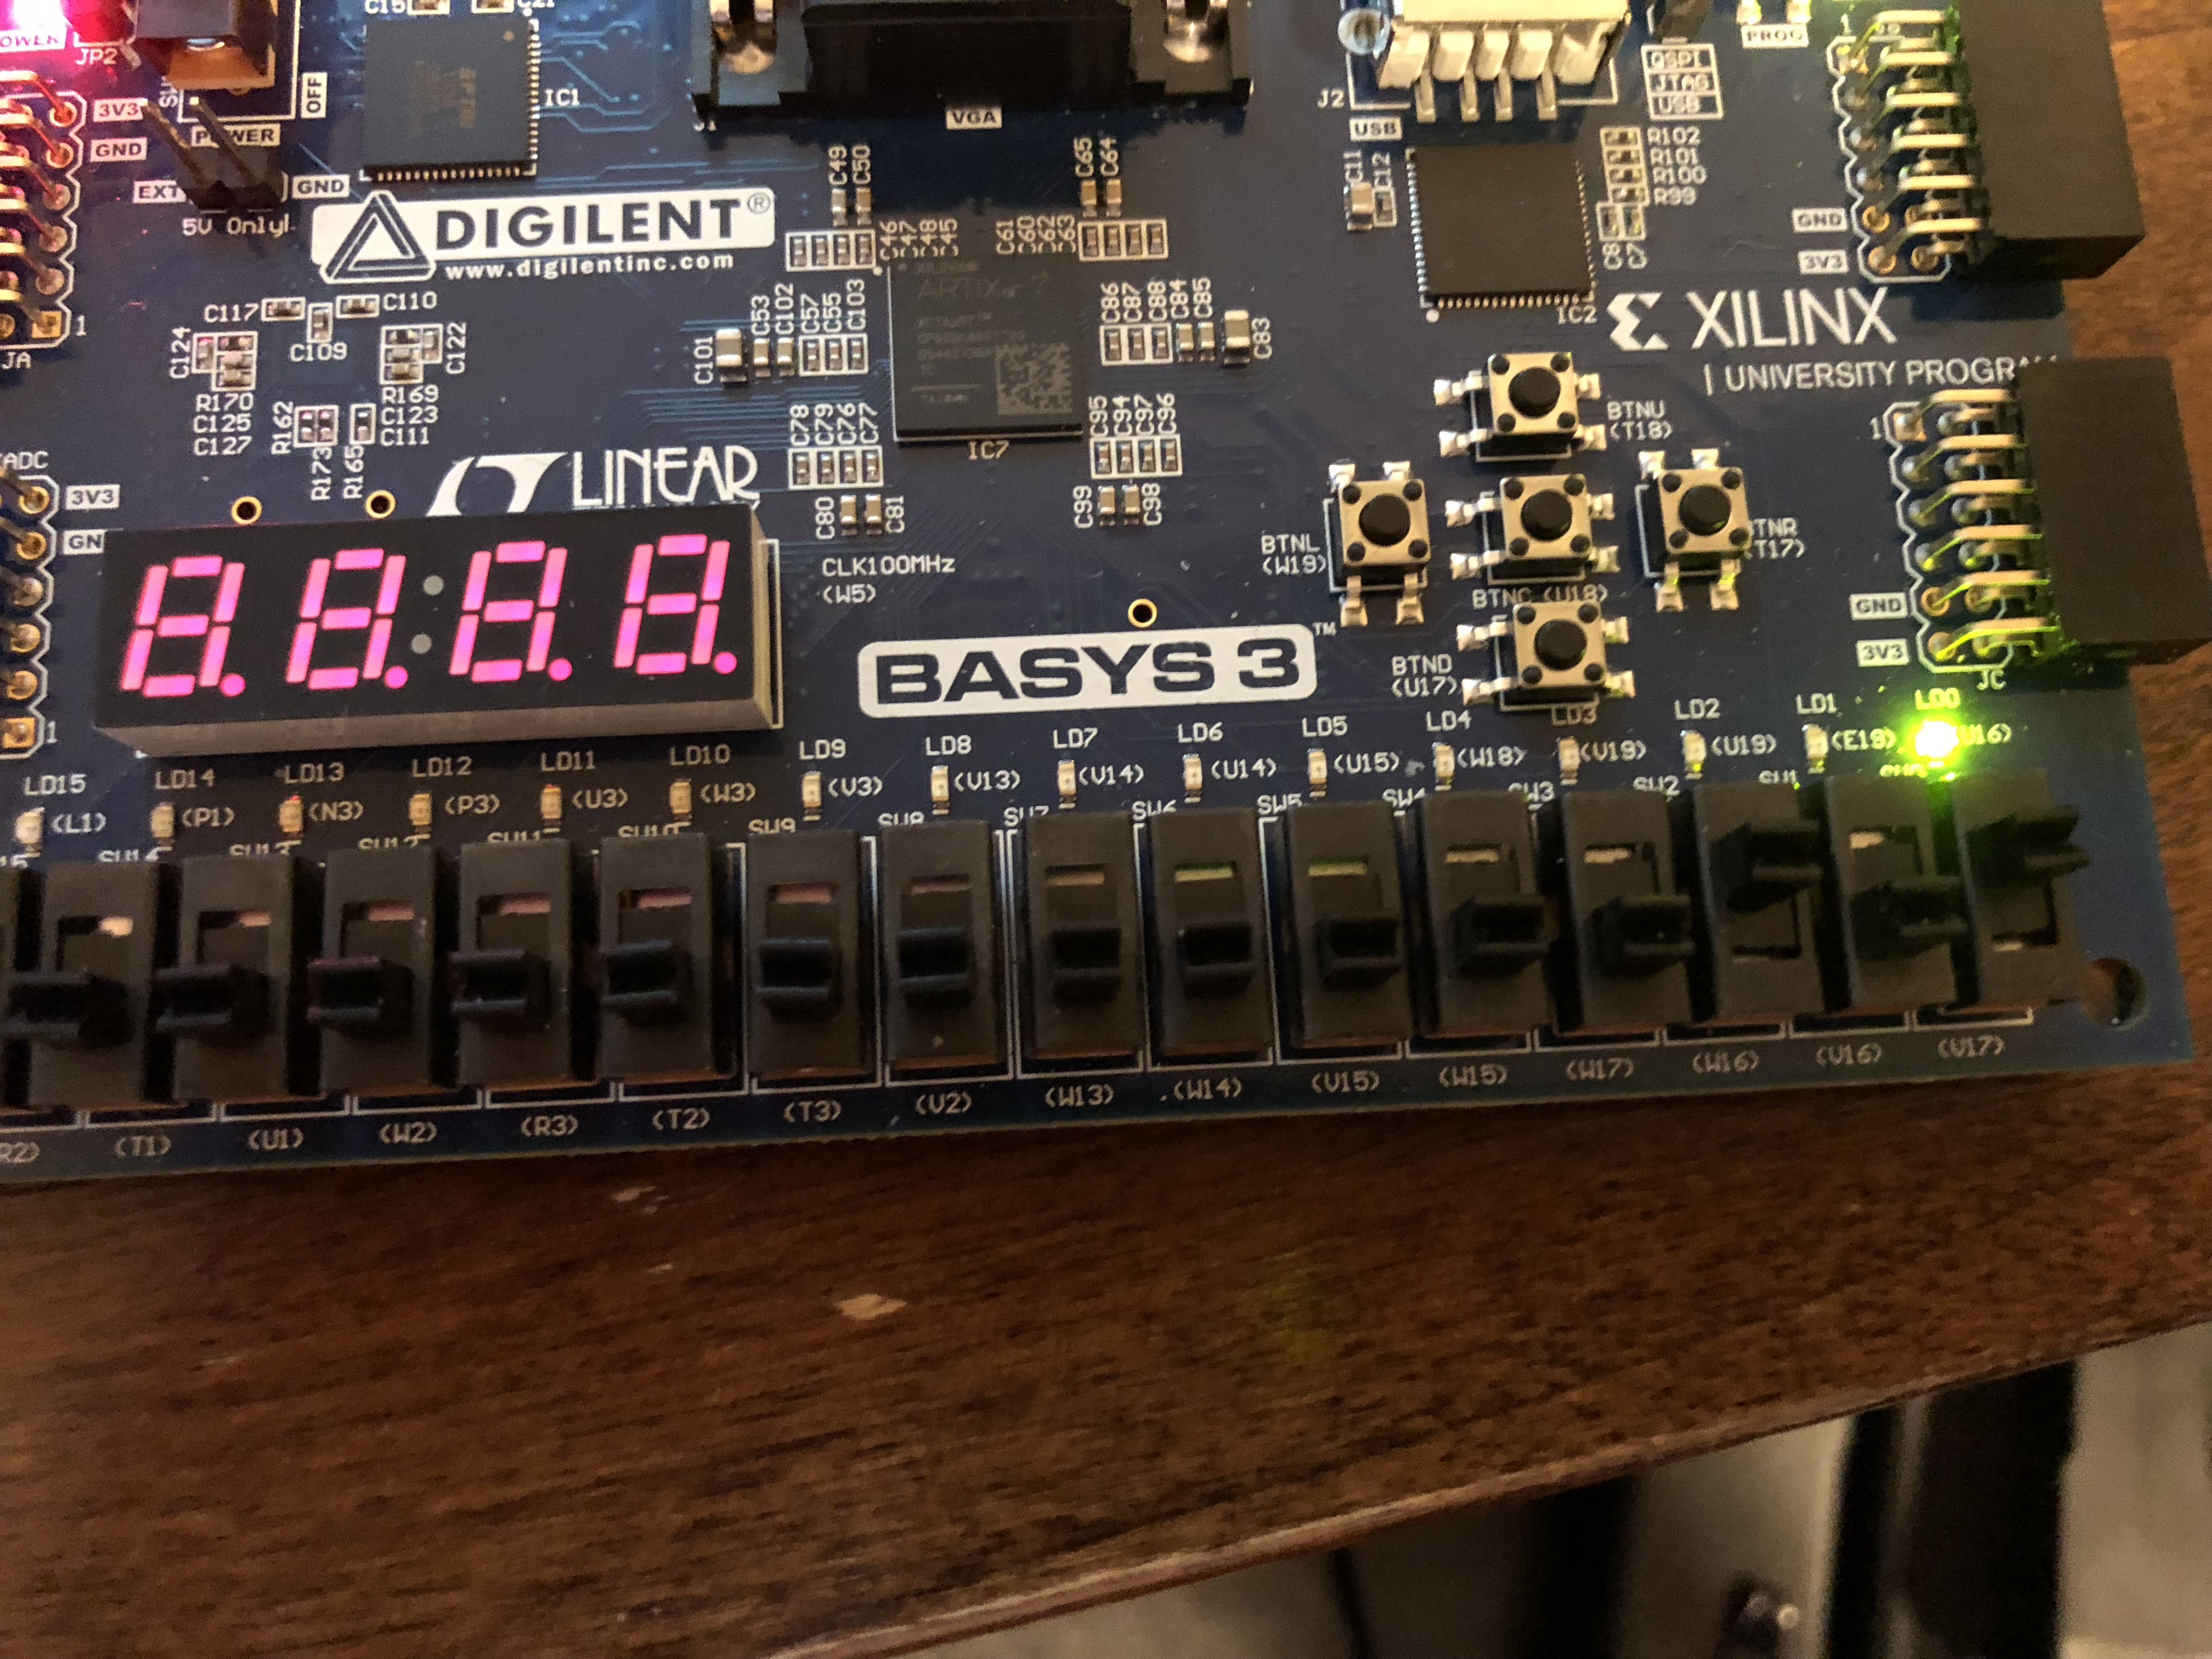
\includegraphics[width=0.5\textwidth]{./images/p3/IMG_3247.jpg}
	\caption{\label{fig:int_res5}FSM is in state 0. 01 AND 01 = 01.}
\end{center}
\end{figure}

\begin{figure}[H]
\begin{center}
	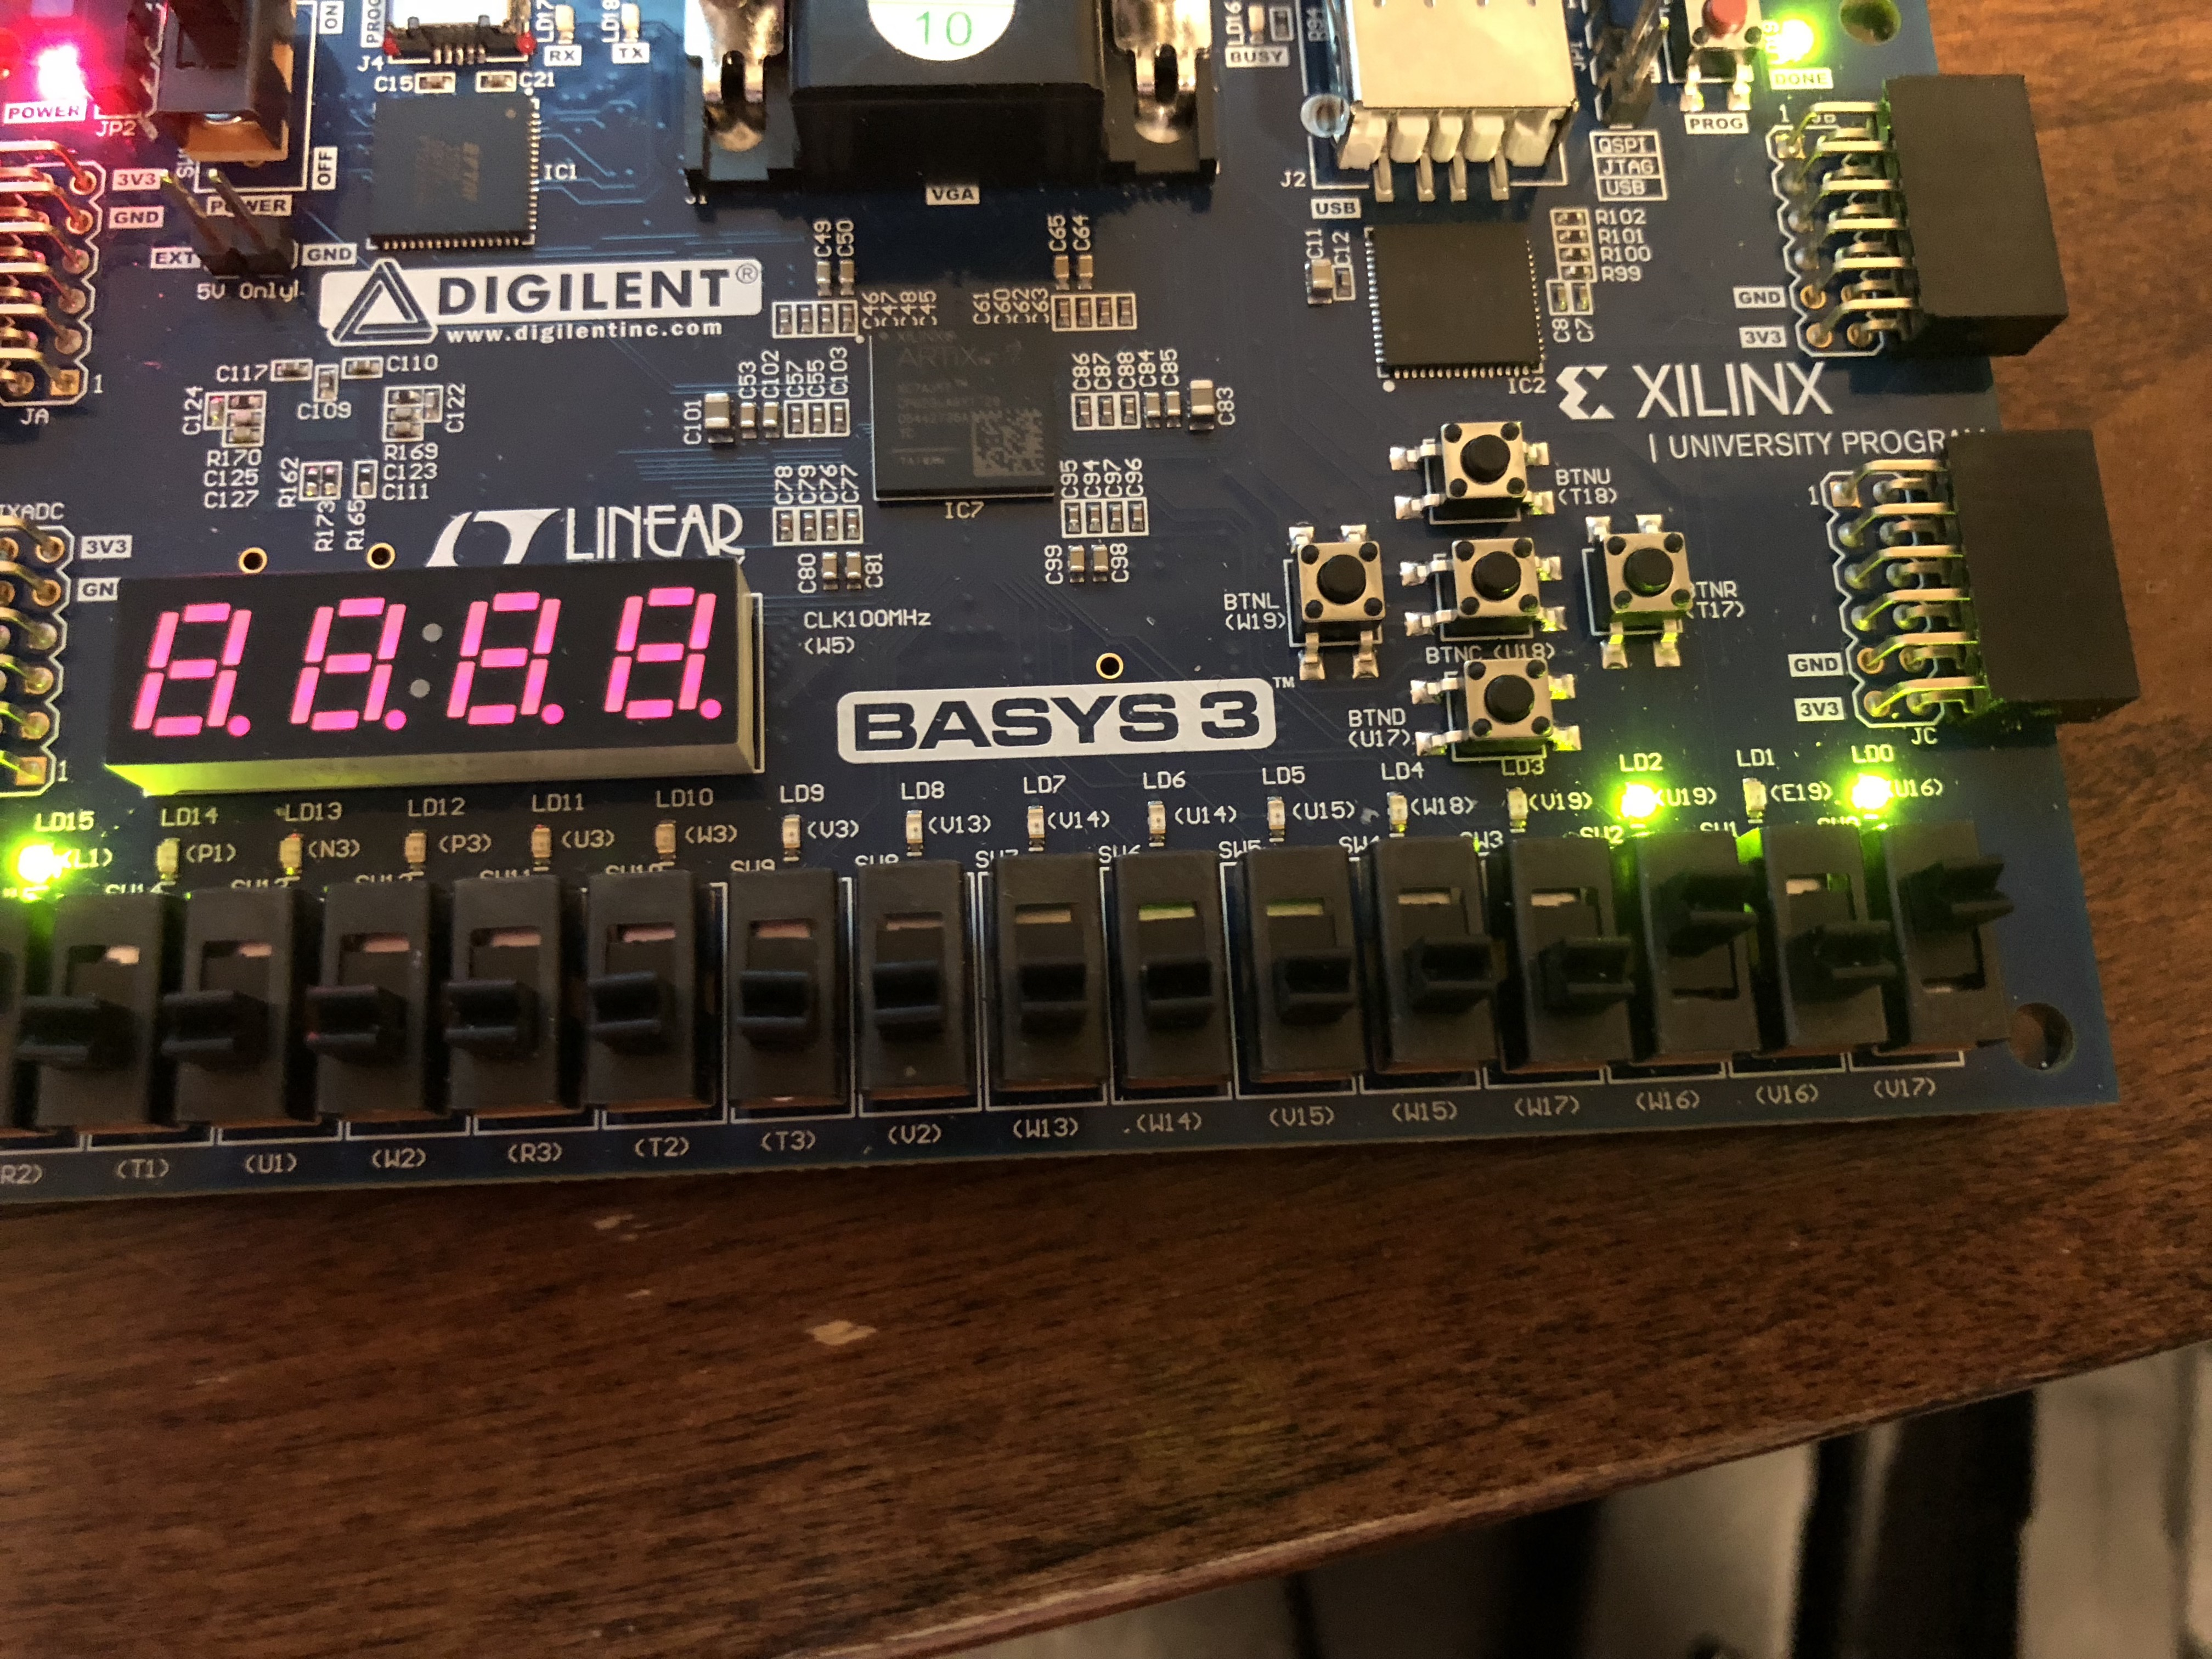
\includegraphics[width=0.5\textwidth]{./images/p3/IMG_0490.jpg}
	\caption{\label{fig:int_res6}FSM is in state 1. 01 OR 01 = 01.}
\end{center}
\end{figure}

\begin{figure}[H]
\begin{center}
	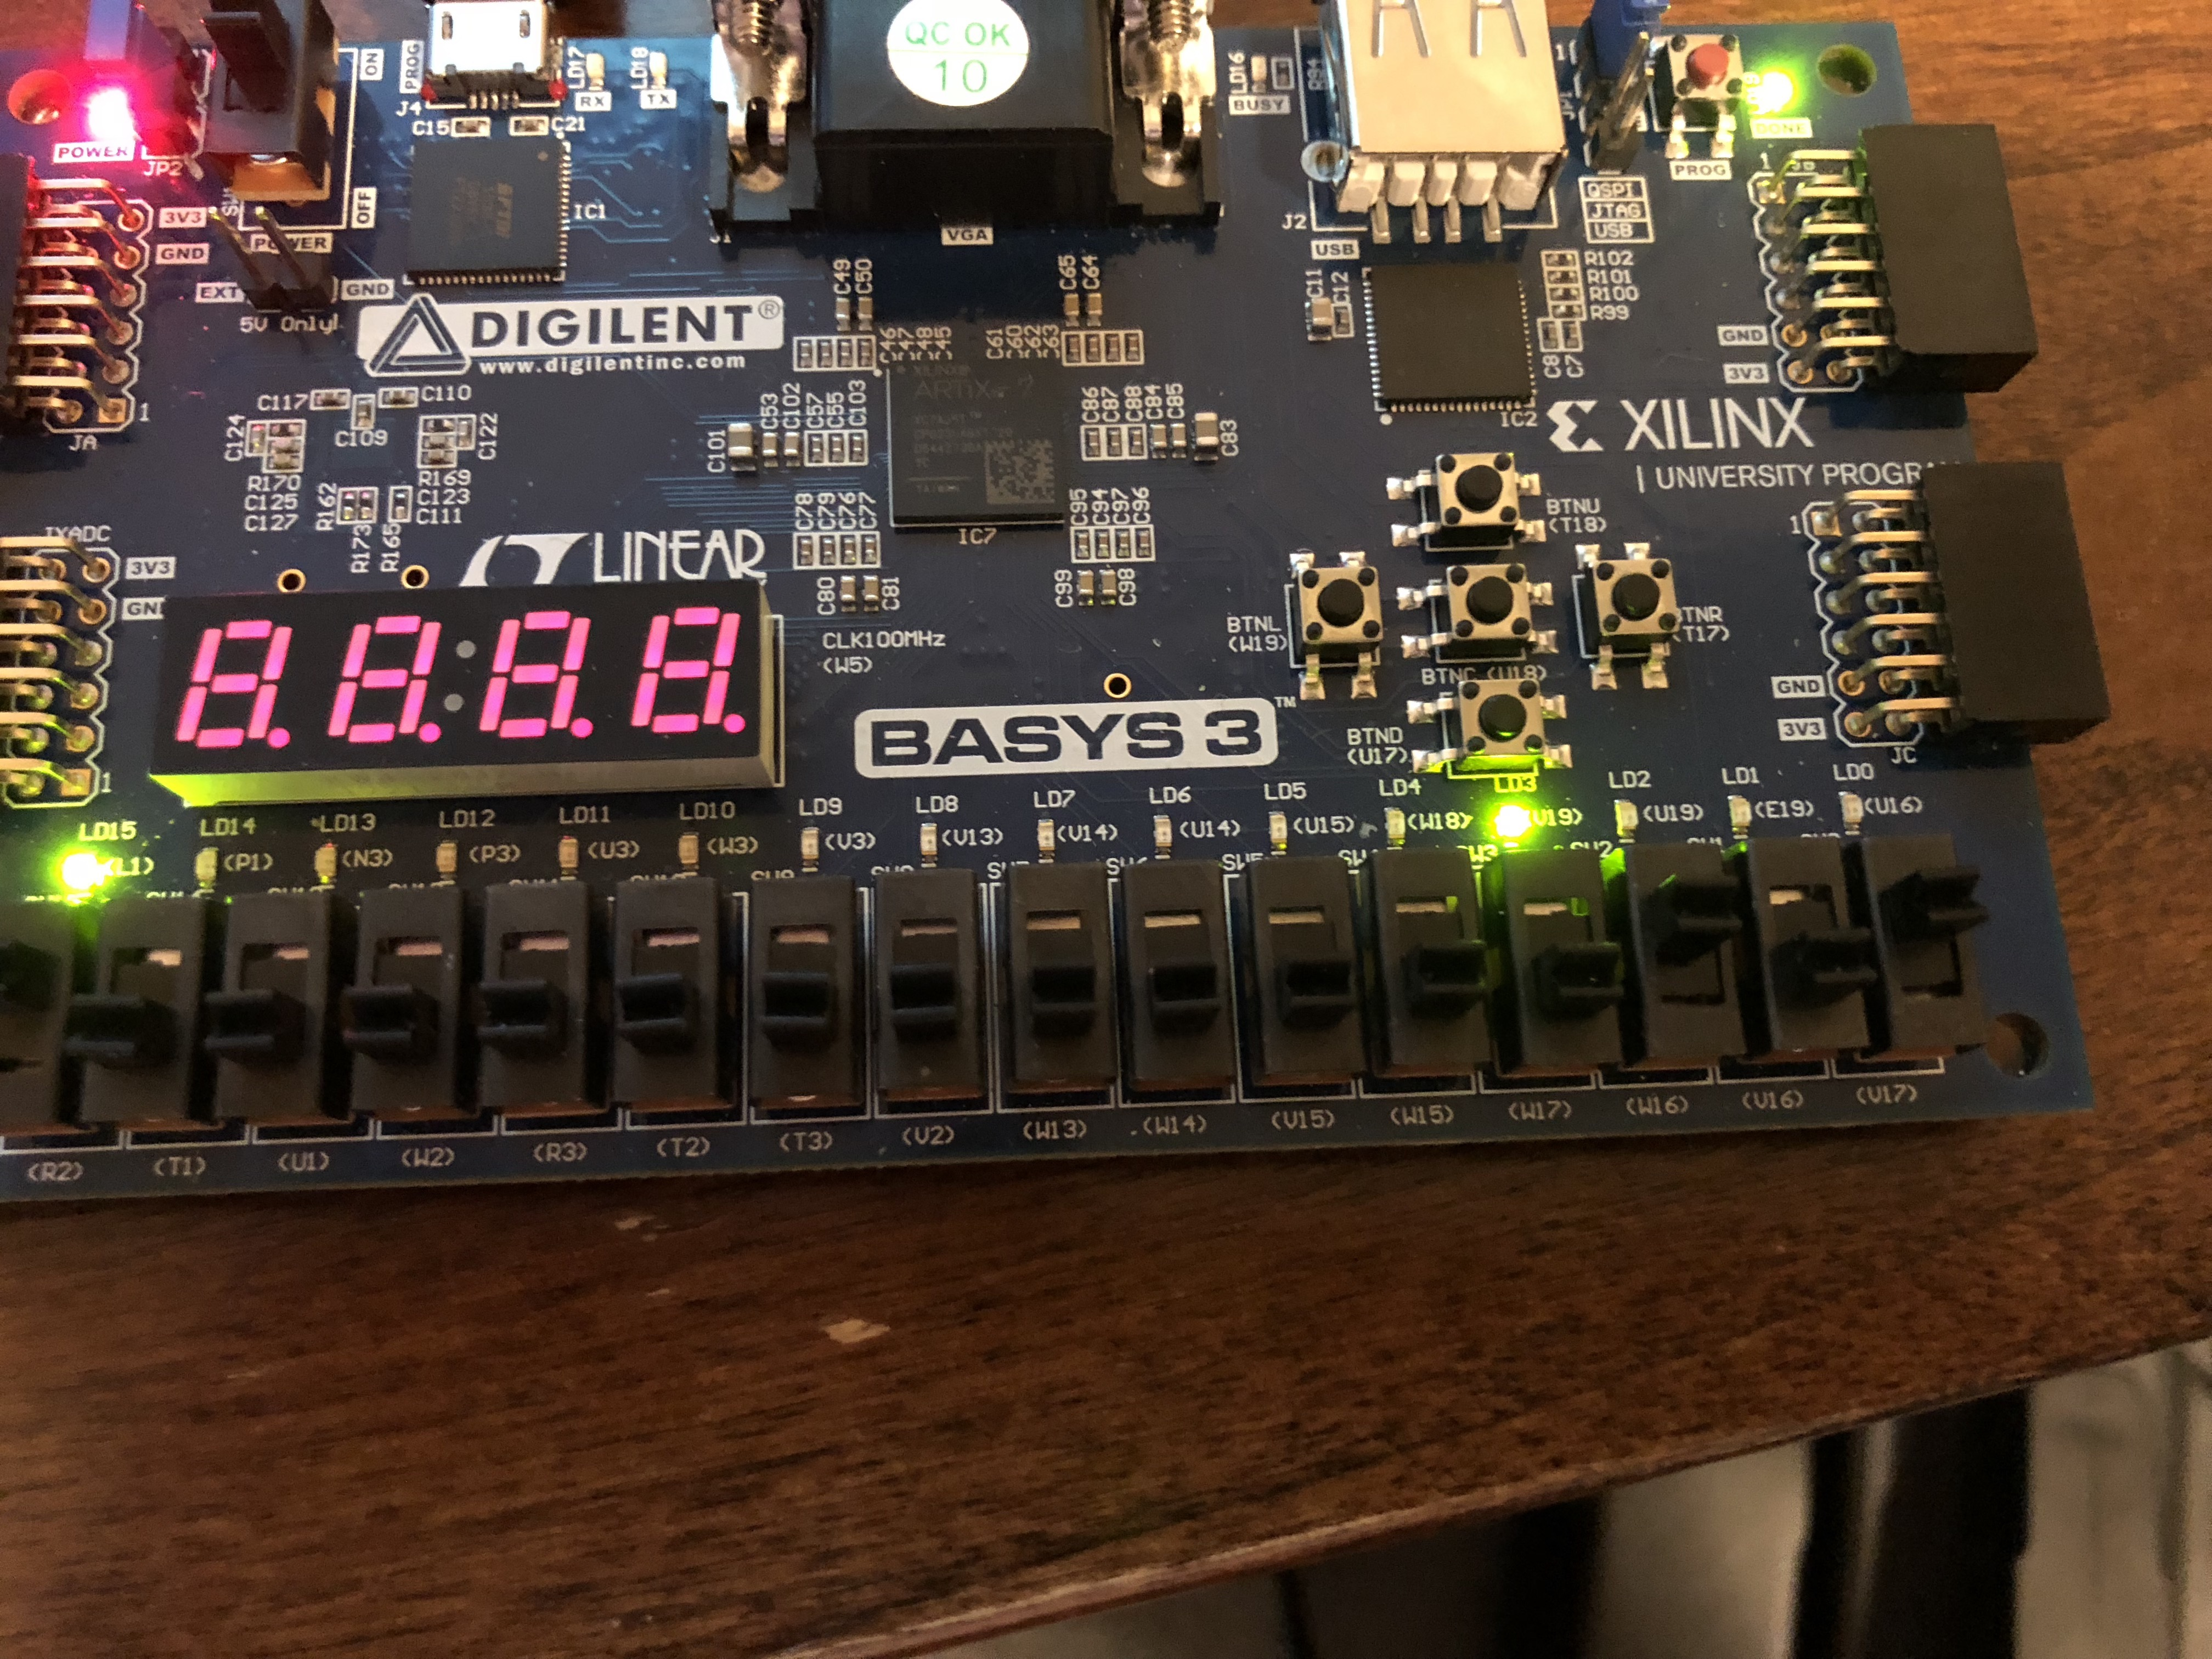
\includegraphics[width=0.5\textwidth]{./images/p3/IMG_7881.jpg}
	\caption{\label{fig:int_res7}FSM is in state 2. 01 shift right by 01 = 00.}
\end{center}
\end{figure}

\begin{figure}[H]
\begin{center}
	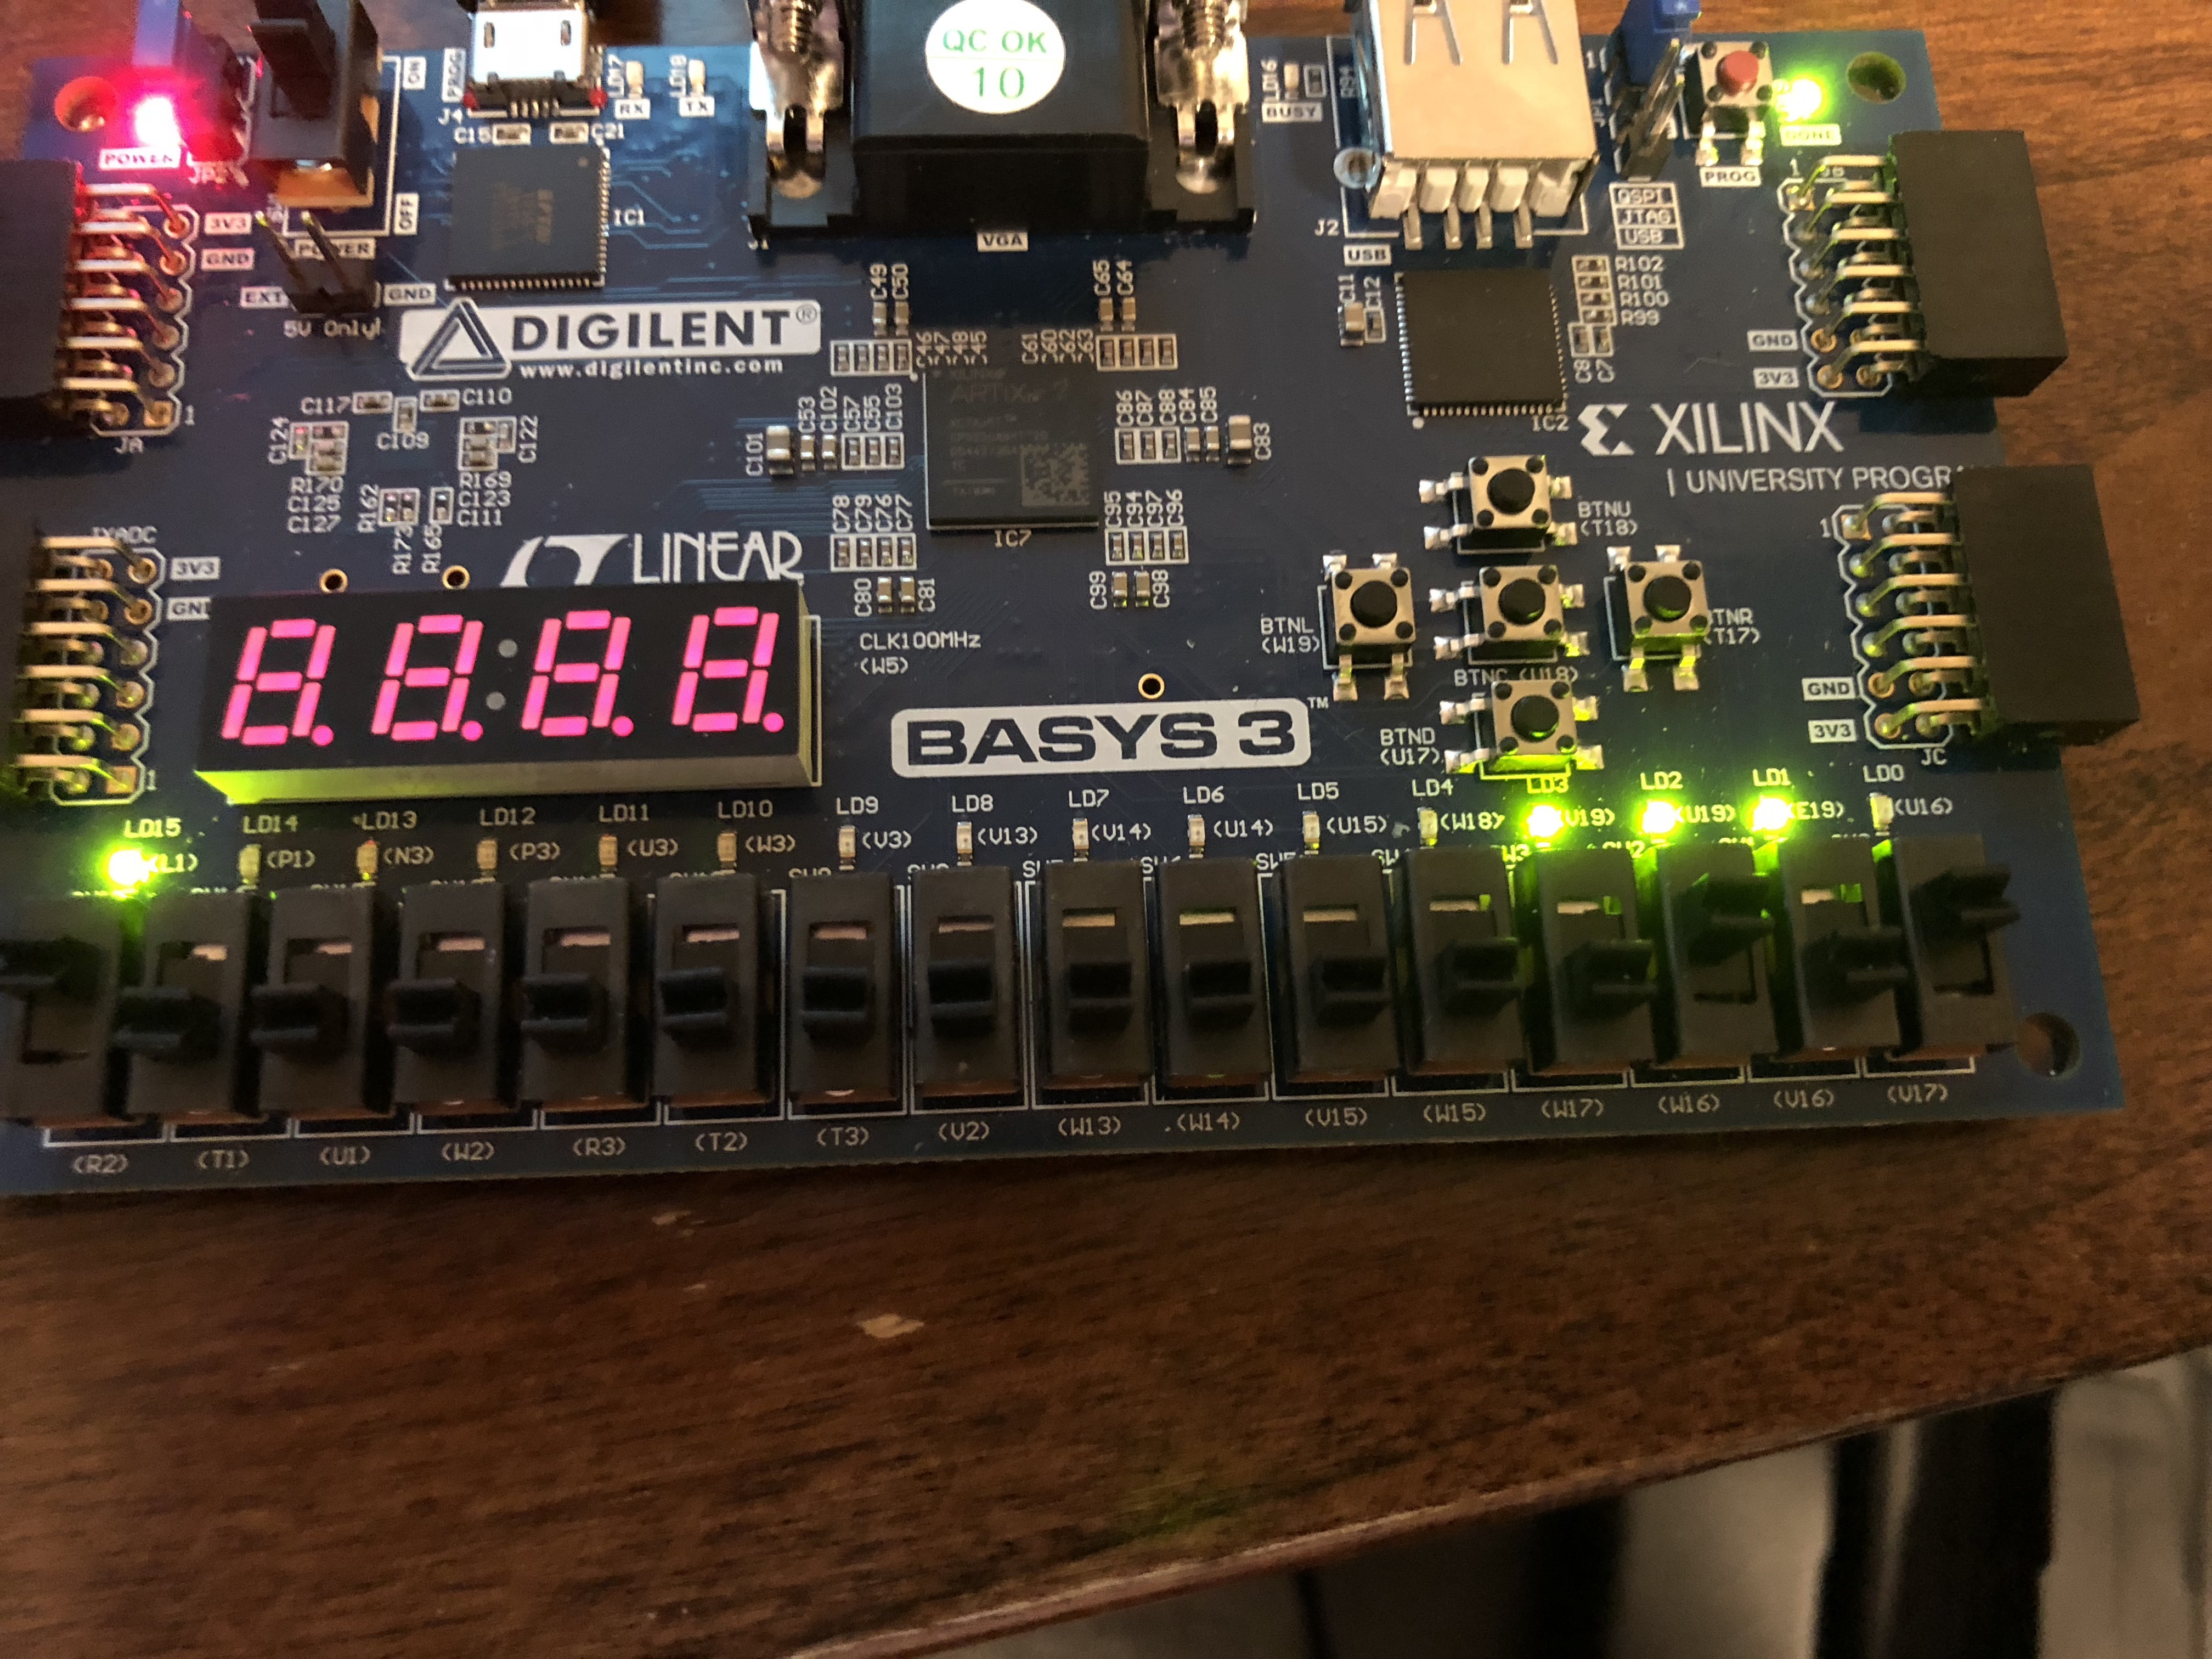
\includegraphics[width=0.5\textwidth]{./images/p3/IMG_1796.jpg}
	\caption{\label{fig:int_res8}FSM is in state 3. 01 shift left by 01 = 10.}
\end{center}
\end{figure}

\section{Conclusion}
This lab gave us experience using a state machine to control a logical unit, and integral part of microprocessor design. The most challenging technical part of this lab was understanding how the different units would fit together, and which inputs or outputs needed to be tied to ports on the board and which could be used as signals.

\pagebreak

\textbf{Appendices}

\begin{appendices}

\section{Problem 1 VHDL Code}

\begin{lstlisting}[language=VHDL]
library IEEE;
use IEEE.STD_LOGIC_1164.ALL;

entity bitwise_and is port(a, b : in STD_LOGIC_VECTOR(1 downto 0); 
	v: out STD_LOGIC_VECTOR(1 downto 0));
end entity bitwise_and;

architecture and_arch of bitwise_and is
begin
    v <= a and b;
end architecture and_arch;

library IEEE;
use IEEE.STD_LOGIC_1164.ALL;

entity bitwise_or is port(c, d : in STD_LOGIC_VECTOR(1 downto 0); 
	x: out STD_LOGIC_VECTOR(1 downto 0));
end entity bitwise_or;

architecture or_arch of bitwise_or is
begin
  x <= c or d;
end architecture or_arch;

library IEEE;
use IEEE.STD_LOGIC_1164.ALL;

entity bitwise_lsr is port(e, f : in STD_LOGIC_VECTOR(1 downto 0); 
	y : out STD_LOGIC_VECTOR(1 downto 0));
end bitwise_lsr;

architecture lsr_arch of bitwise_lsr is
begin
    process(e, f)
    begin
        case f is
        when "00" =>
            y <= e;
        when "01" =>
            if(e = "00") then y <= "00";
            elsif(e = "01") then y <= "00";
            else y <= "01";
            end if;
        when others =>
            y <= "00";
        end case;
     end process;
end lsr_arch;

library IEEE;
use IEEE.STD_LOGIC_1164.ALL;

entity bitwise_lsl is port(g, h : in STD_LOGIC_VECTOR(1 DOWNTO 0); 
	z : out STD_LOGIC_VECTOR(1 downto 0));
end bitwise_lsl;

architecture lsl_arch of bitwise_lsl is
begin
    process(g, h)
    begin
        case h is
        when "00" =>
            z <= g;
        when "01" =>
            if(g = "11") then z <= "10";
            elsif(g = "01") then z <="10";
            else z <= "00";
            end if;
        when others =>
            z <= "00";
        end case;
    end process;
end lsl_arch;

library IEEE;
use IEEE.STD_LOGIC_1164.ALL;

entity ArithmeticLogicUnit is
    Port ( in1 : in STD_LOGIC_VECTOR(1 downto 0);
           in2 : in STD_LOGIC_VECTOR(1 downto 0);
           sel : in STD_LOGIC_VECTOR(1 downto 0);
           output : out STD_LOGIC_VECTOR(1 downto 0));
end ArithmeticLogicUnit;

architecture Behavioral of ArithmeticLogicUnit is
component bitwise_and is port(a, b : in STD_LOGIC_VECTOR(1 downto 0); 
	v : out STD_LOGIC_VECTOR(1 downto 0));
end component bitwise_and;

component bitwise_or is port(c, d : in STD_LOGIC_VECTOR(1 downto 0); 
	x : out STD_LOGIC_VECTOR(1 downto 0));
end component bitwise_or;

component bitwise_lsr is port(e, f : in STD_LOGIC_VECTOR(1 downto 0); 
	y : out STD_LOGIC_VECTOR(1 downto 0));
end component bitwise_lsr;

component bitwise_lsl is port(g, h : in STD_LOGIC_VECTOR(1 DOWNTO 0); 
	z : out STD_LOGIC_VECTOR(1 downto 0));
end component bitwise_lsl;

signal and_output : STD_LOGIC_VECTOR(1 downto 0);
signal or_output : STD_LOGIC_VECTOR(1 downto 0);
signal lsr_output : STD_LOGIC_VECTOR(1 downto 0);
signal lsl_output : STD_LOGIC_VECTOR(1 downto 0);

begin
    and_comp : bitwise_and port map(in1, in2, and_output);
    or_comp : bitwise_or port map(in1, in2, or_output);
    lsr_comp : bitwise_lsr port map(in1, in2, lsr_output);
    lsl_comp : bitwise_lsl port map(in1, in2, lsl_output);
    
    process(sel)
    begin
        case sel is
            when "00" =>
                output <= and_output;
            when "01" =>
                output <= or_output;
            when "10" =>
                output <= lsr_output;
            when "11" =>
                output <= lsl_output;
        end case;
    end process;                

end Behavioral;
\end{lstlisting}

\section{Problem 1 Constraints File}
\begin{center}
\begin{figure}[H]
	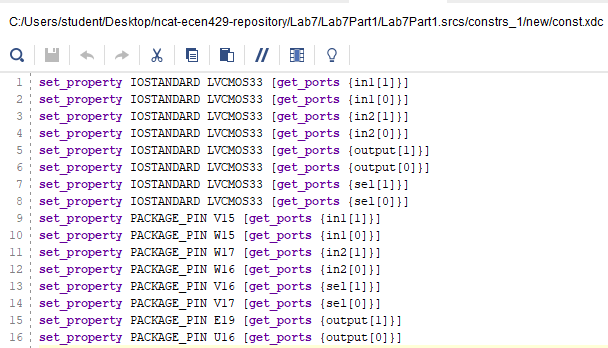
\includegraphics[scale=1]{./images/Lab7Part1Const.png}
	\caption{\label{fig:Prob1Const}Constraints file for Problem 1.}
\end{figure}
\end{center}

\section{Problem 2 VHDL Code}
\begin{lstlisting}[language=VHDL]
library IEEE;
use IEEE.STD_LOGIC_1164.ALL;
use IEEE.NUMERIC_STD.ALL;

entity Clockdivider is
     port(clk : in std_logic;
          start_timer : in std_logic;
	  FastClock,MediumClock,SlowClock, led0 : out std_logic);
end Clockdivider;

architecture clockdivider_arch of Clockdivider is

signal slowClock_sig : STD_LOGIC;

begin
    process  
    variable cnt :	
    		std_logic_vector(26 downto 0):= "000000000000000000000000000";
    begin					 
        wait until ((clk'EVENT) AND (clk = '1'));
	       
		if (start_timer = '1') then
	       cnt := "000000000000000000000000000";
	    else  
           cnt := STD_LOGIC_VECTOR(unsigned(cnt) + 1);
	    end if;

   	    FastClock <= cnt(22);
   	    MediumClock <= cnt(24);	
   	    SlowClock <= cnt(26);
        slowClock_sig <= cnt(26);
	
        if (slowClock_sig = '1') then
		  led0 <= '1';
	    else
		  led0 <= '0';
	    end if;
	end process;
end clockdivider_arch;


library IEEE;
use IEEE.STD_LOGIC_1164.ALL;

entity FSM is
    Port ( clk : in STD_LOGIC;
           enable : in STD_LOGIC;
           reset : in STD_LOGIC;
           output_sel : out STD_LOGIC_VECTOR(1 downto 0);
           clock_led : out STD_LOGIC);
end FSM;

architecture Behavioral of FSM is
component Clockdivider is 
          Port (clk : in std_logic;
          start_timer : in std_logic;
	      FastClock,MediumClock,SlowClock, led0 : out std_logic);
end component Clockdivider;

signal fastclocksig :STD_LOGIC;
signal medclocksig :STD_LOGIC;
signal slowclocksig :STD_LOGIC;
signal current_state : STD_LOGIC_VECTOR(1 downto 0) := "00";

begin
    clockDiv : Clockdivider port map(clk, reset, fastclocksig, medclocksig, 
    		slowclocksig, clock_led);
    
    process(slowclocksig, reset)
    begin
        if(reset = '1') then
            current_state <= "00";
            output_sel <= "00";
        end if;
        if(slowclocksig'event and (slowclocksig = '1')) then
            if(enable = '1') then
            case current_state is
                when "00" =>
                    current_state <= "01";
                    output_sel <= "01";
                when "01" =>
                    current_state <= "10";
                    output_sel <= "10";
                when "10" =>
                    current_state <= "11";
                    output_sel <= "11";
                when "11" =>
                    current_state <= "00";
                    output_sel <= "00";
            end case;
            else
                current_state <= "00";
                output_sel <= "00";
            end if;
        end if;
    end process;
    
    output_sel <= current_state;
end Behavioral;
\end{lstlisting}

\section{Problem 2 Constraints File}
\begin{center}
\begin{figure}[H]
	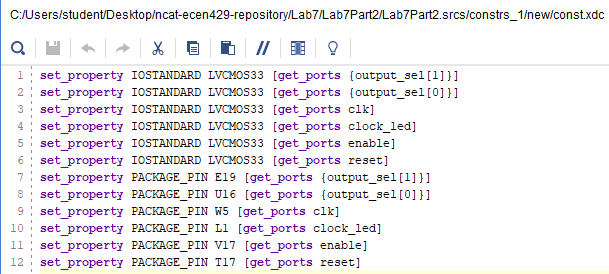
\includegraphics[scale=1]{./images/Lab7Part2Const.png}
	\caption{\label{fig:Prob1Const}Constraints file for Problem 2.}
\end{figure}
\end{center}

\section{Problem 3 VHDL Code}
\begin{lstlisting}[language=VHDL]
library IEEE;
use IEEE.STD_LOGIC_1164.ALL;

entity TopLevelDesign is
    Port ( input1 : in STD_LOGIC_VECTOR(1 downto 0);
           input2 : in STD_LOGIC_VECTOR(1 downto 0);
           clk : in STD_LOGIC;
           enable : in STD_LOGIC;
           reset : in STD_LOGIC;
           output : out STD_LOGIC_VECTOR(1 downto 0);
           clock_led : out STD_LOGIC;
           operation : out STD_LOGIC_VECTOR(1 downto 0));
end TopLevelDesign;

architecture Behavioral of TopLevelDesign is
component FSM is
    Port ( clk : in STD_LOGIC;
           enable : in STD_LOGIC;
           reset : in STD_LOGIC;
           output_sel : out STD_LOGIC_VECTOR(1 downto 0);
           clock_led : out STD_LOGIC);
end component FSM;

component ArithmeticLogicUnit is
    Port ( in1 : in STD_LOGIC_VECTOR(1 downto 0);
           in2 : in STD_LOGIC_VECTOR(1 downto 0);
           sel : in STD_LOGIC_VECTOR(1 downto 0);
           output : out STD_LOGIC_VECTOR(1 downto 0));
end component ArithmeticLogicUnit;

signal select_signal : STD_LOGIC_VECTOR(1 downto 0);

begin
    stateMachine : FSM 
    		port map(clk, enable, reset, select_signal, clock_led);
    logicUnit : ArithmeticLogicUnit 
    		port map(input1, input2, select_signal, output);
    operation <= select_signal;
end Behavioral;
\end{lstlisting}

\section{Problem 3 Constraints File}
\begin{center}
\begin{figure}[H]
	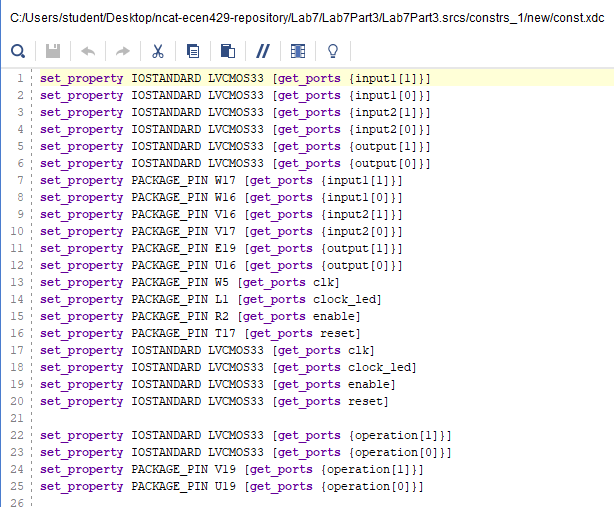
\includegraphics[scale=1]{./images/Lab7Part3Const.png}
	\caption{\label{fig:Prob1Const}Constraints file for Problem 3.}
\end{figure}
\end{center}

\end{appendices}
\end{document}
